\documentclass[11pt,xcolor={dvipsnames}, aspectratio=169]{beamer}
\usetheme[
%%% option passed to the outer theme
%    progressstyle=fixedCircCnt,   % fixedCircCnt, movingCircCnt (moving is deault)
  ]{Feather}
  
% If you want to change the colors of the various elements in the theme, edit and uncomment the following lines

% Change the bar colors:
\setbeamercolor{Feather}{fg=NavyBlue!20,bg=NavyBlue}
%
%% Change the color of the structural elements:
\setbeamercolor{structure}{fg=NavyBlue}
%
%% Change the frame title text color:
\setbeamercolor{frametitle}{fg=black!5}
%
%% Change the normal text colors:
\setbeamercolor{normal text}{fg=black!75,bg=gray!5}
%
%%% Change the block title colors
\setbeamercolor{block title}{use=Feather,bg=Feather.fg, fg=black!90} 


% Change the logo in the upper right circle:
%\renewcommand{\logofile}{example-grid-100x100pt} 
%% This is an image that comes with the LaTeX installation
% Adjust scale of the logo w.r.t. the circle; default is 0.875
% \renewcommand{\logoscale}{0.55}

% Change the background image on the title and final page.
% It stretches to fill the entire frame!
% \renewcommand{\backgroundfile}{example-grid-100x100pt}

%-------------------------------------------------------
% INCLUDE PACKAGES
%-------------------------------------------------------

\usepackage{amsmath}
\usepackage{amsfonts}
\usepackage{pgfplots}
\usepackage{filecontents}
\usepackage{caption}
\usepackage{subcaption}
\usepackage[dvipsnames]{xcolor}

% If you want to change the colors of the various elements in the theme, edit and uncomment the following lines

% Change the bar colors:
%\setbeamercolor{Feather}{fg=red!20,bg=red}

% Change the color of the structural elements:
%\setbeamercolor{structure}{fg=red}

% Change the frame title text color:
%\setbeamercolor{frametitle}{fg=blue}

% Change the normal text color background:
%\setbeamercolor{normal text}{fg=black,bg=gray!10}

%-------------------------------------------------------
% INCLUDE PACKAGES
%-------------------------------------------------------

\usepackage[utf8]{vietnam}
\usepackage{amsmath}
\usepackage{algorithm}
\usepackage[noend]{algpseudocode}
\usepackage{geometry}
\usepackage{float}
\usepackage{helvet}


\captionsetup{labelformat=empty,labelsep=none}

% \usepackage{helvet}

%% Load different font packages to use different fonts
%% e.g. using Linux Libertine, Linux Biolinum and Inconsolata
% \usepackage{libertine}
% \usepackage{zi4}

%% e.g. using Carlito and Caladea


%% e.g. using Venturis ADF Serif and Sans
% \usepackage{venturis}

%-------------------------------------------------------
% DEFFINING AND REDEFINING COMMANDS
%-------------------------------------------------------

% colored hyperlinks
\newcommand{\chref}[2]{
  \href{#1}{{\usebeamercolor[bg]{Feather}#2}}
}

%-------------------------------------------------------
% INFORMATION IN THE TITLE PAGE
%-------------------------------------------------------

\title[] % [] is optional - is placed on the bottom of the sidebar on every slide
{ % is placed on the title page
      \textbf{Sử dụng mạng Bayesian ước lượng tài nguyên khả dụng cho bài toán lập lịch trong môi trường \\
      Cloud Computing}
}


\author[Quang Khanh]
{     Sinh viên thực hiện: Trương Quang Khánh \\
	 Lớp: KSTN-CNTT Khóa 62 \\
      { Giảng viên hướng dẫn: PSG. Nguyễn Bình Minh}
}

\institute[]
{%
\vspace{0.5cm}
	{\centering 
\includegraphics[scale=0.3]{images/hustlogo.png}}\\
	{\centering Viện Công nghệ Thông tin và Truyền thông}
%      Đại học Bách khoa Hà Nội\\
%	  Viện Công nghệ Thông tin và Truyền thông
}

\date{Ngày 9 tháng 7 năm 2021}

%-------------------------------------------------------
% THE BODY OF THE PRESENTATION
%-------------------------------------------------------

\setbeamertemplate{section in toc}[sections numbered]

\setbeamertemplate{footline}{
    \hbox{%
    \begin{beamercolorbox}[wd=\paperwidth,ht=3ex,dp=1.5ex,leftskip=2ex,rightskip=2ex]{page footer}%
        \usebeamerfont{title in head/foot}%
        \insertshorttitle \hfill
            \color{white}{\insertsection} \hfill
    \end{beamercolorbox}}%
}

\AtBeginSection[]{
  \begin{frame}
  \vfill
  \centering
  \begin{beamercolorbox}[sep=8pt,center,shadow=true,rounded=true]{title}
    \usebeamerfont{title}\insertsectionnumber ~. \insertsectionhead\par%
  \end{beamercolorbox}
  \vfill
  \end{frame}
}

\begin{document}

%-------------------------------------------------------
% THE TITLEPAGE
%-------------------------------------------------------

{\1% % this is the name of the PDF file for the background
\begin{frame}[plain,noframenumbering] % the plain option removes the header from the title page, noframenumbering removes the numbering of this frame only
  \titlepage % call the title page information from above
\end{frame}}


\begin{frame}{Nội dung}{}
\tableofcontents
\end{frame}

\section{Giới thiệu chung}

\begin{frame}
{Sự xuất hiện của Cloud Computing}
\begin{figure}
	\centering
	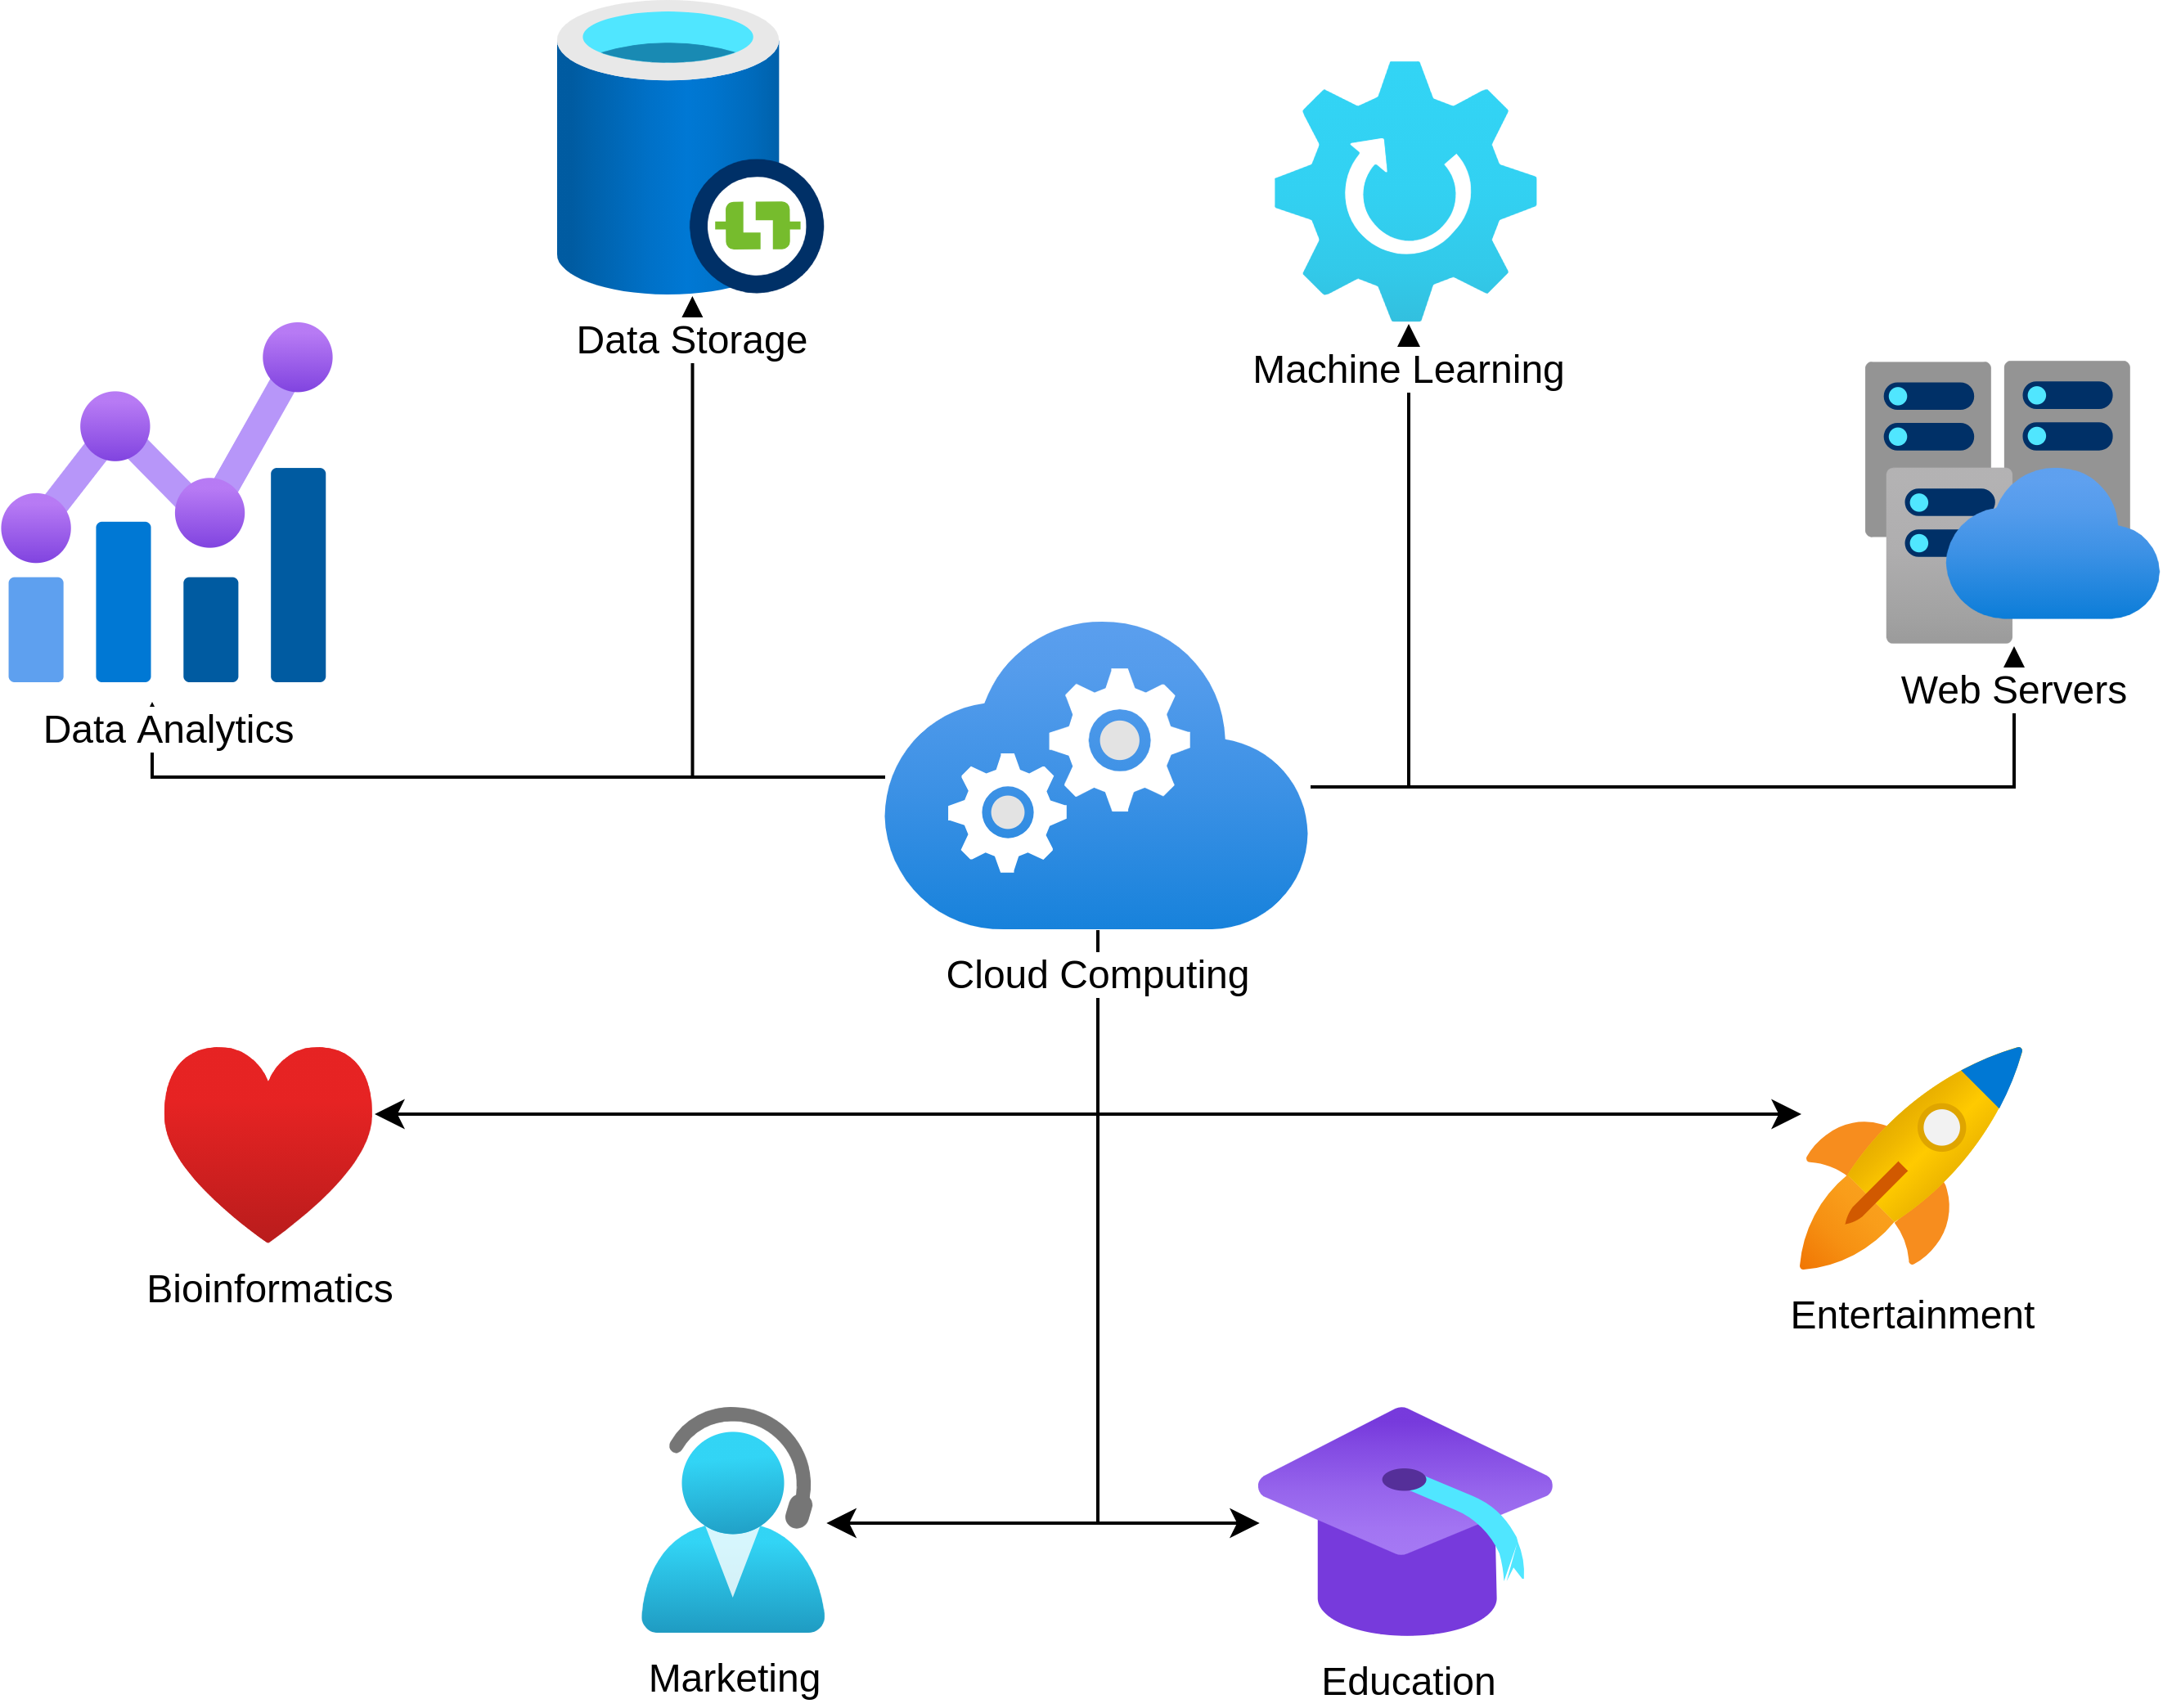
\includegraphics[scale=0.5]{images/cloud_computing_applications.png}
\end{figure}
\end{frame}

%\begin{frame}
%{Cloud Computing}
%% Giới thiệu về Cloud Computing là gì
%\begin{block}
%{Data Center}
%Là hệ thống các máy chủ trong công ty, tổ chức nhằm phục vụ mục đích lưu trữ và truy cập dữ liệu, cung cấp tiện ích tới người dùng (nhân viên, ...) thông qua mạng nội bộ. Việc xây dựng, bảo trì hệ thống được thực hiện bởi nội bộ công ty.
%\end{block}
%\pause
%\begin{block}
%{Cloud}
%Là phiên bản 'từ xa' của Data center, được đặt ở nơi nào đó không phải là ở công ty, tổ chức, người dùng truy cập thông qua internet. Việc quản lý, xây dựng được thực hiện bởi nhà cung cấp dịch vụ cloud.
%\end{block} 
%\end{frame}


\begin{frame}
{Vấn đề lập lịch trong hệ thống Cloud}
% Tại sao cần lập lịch trong hệ thống Cloud
\begin{minipage}[t]{0.48\linewidth}
	\begin{block}
	{Luồng hoạt động}
	\begin{enumerate}
		\item Người dùng gửi các tasks đến hệ thống
		\item Các tasks được đưa đến hàng đợi cho đến khi được lập lịch
		\item Bộ lập lịch tìm các máy tính phù hợp cho các tasks
		\item Chuyển các tasks đến các máy tính và thực thi
	\end{enumerate}
	\end{block}
\end{minipage}
\hfill
\begin{minipage}[t]{0.48\linewidth}
	\begin{figure}
		\centering
		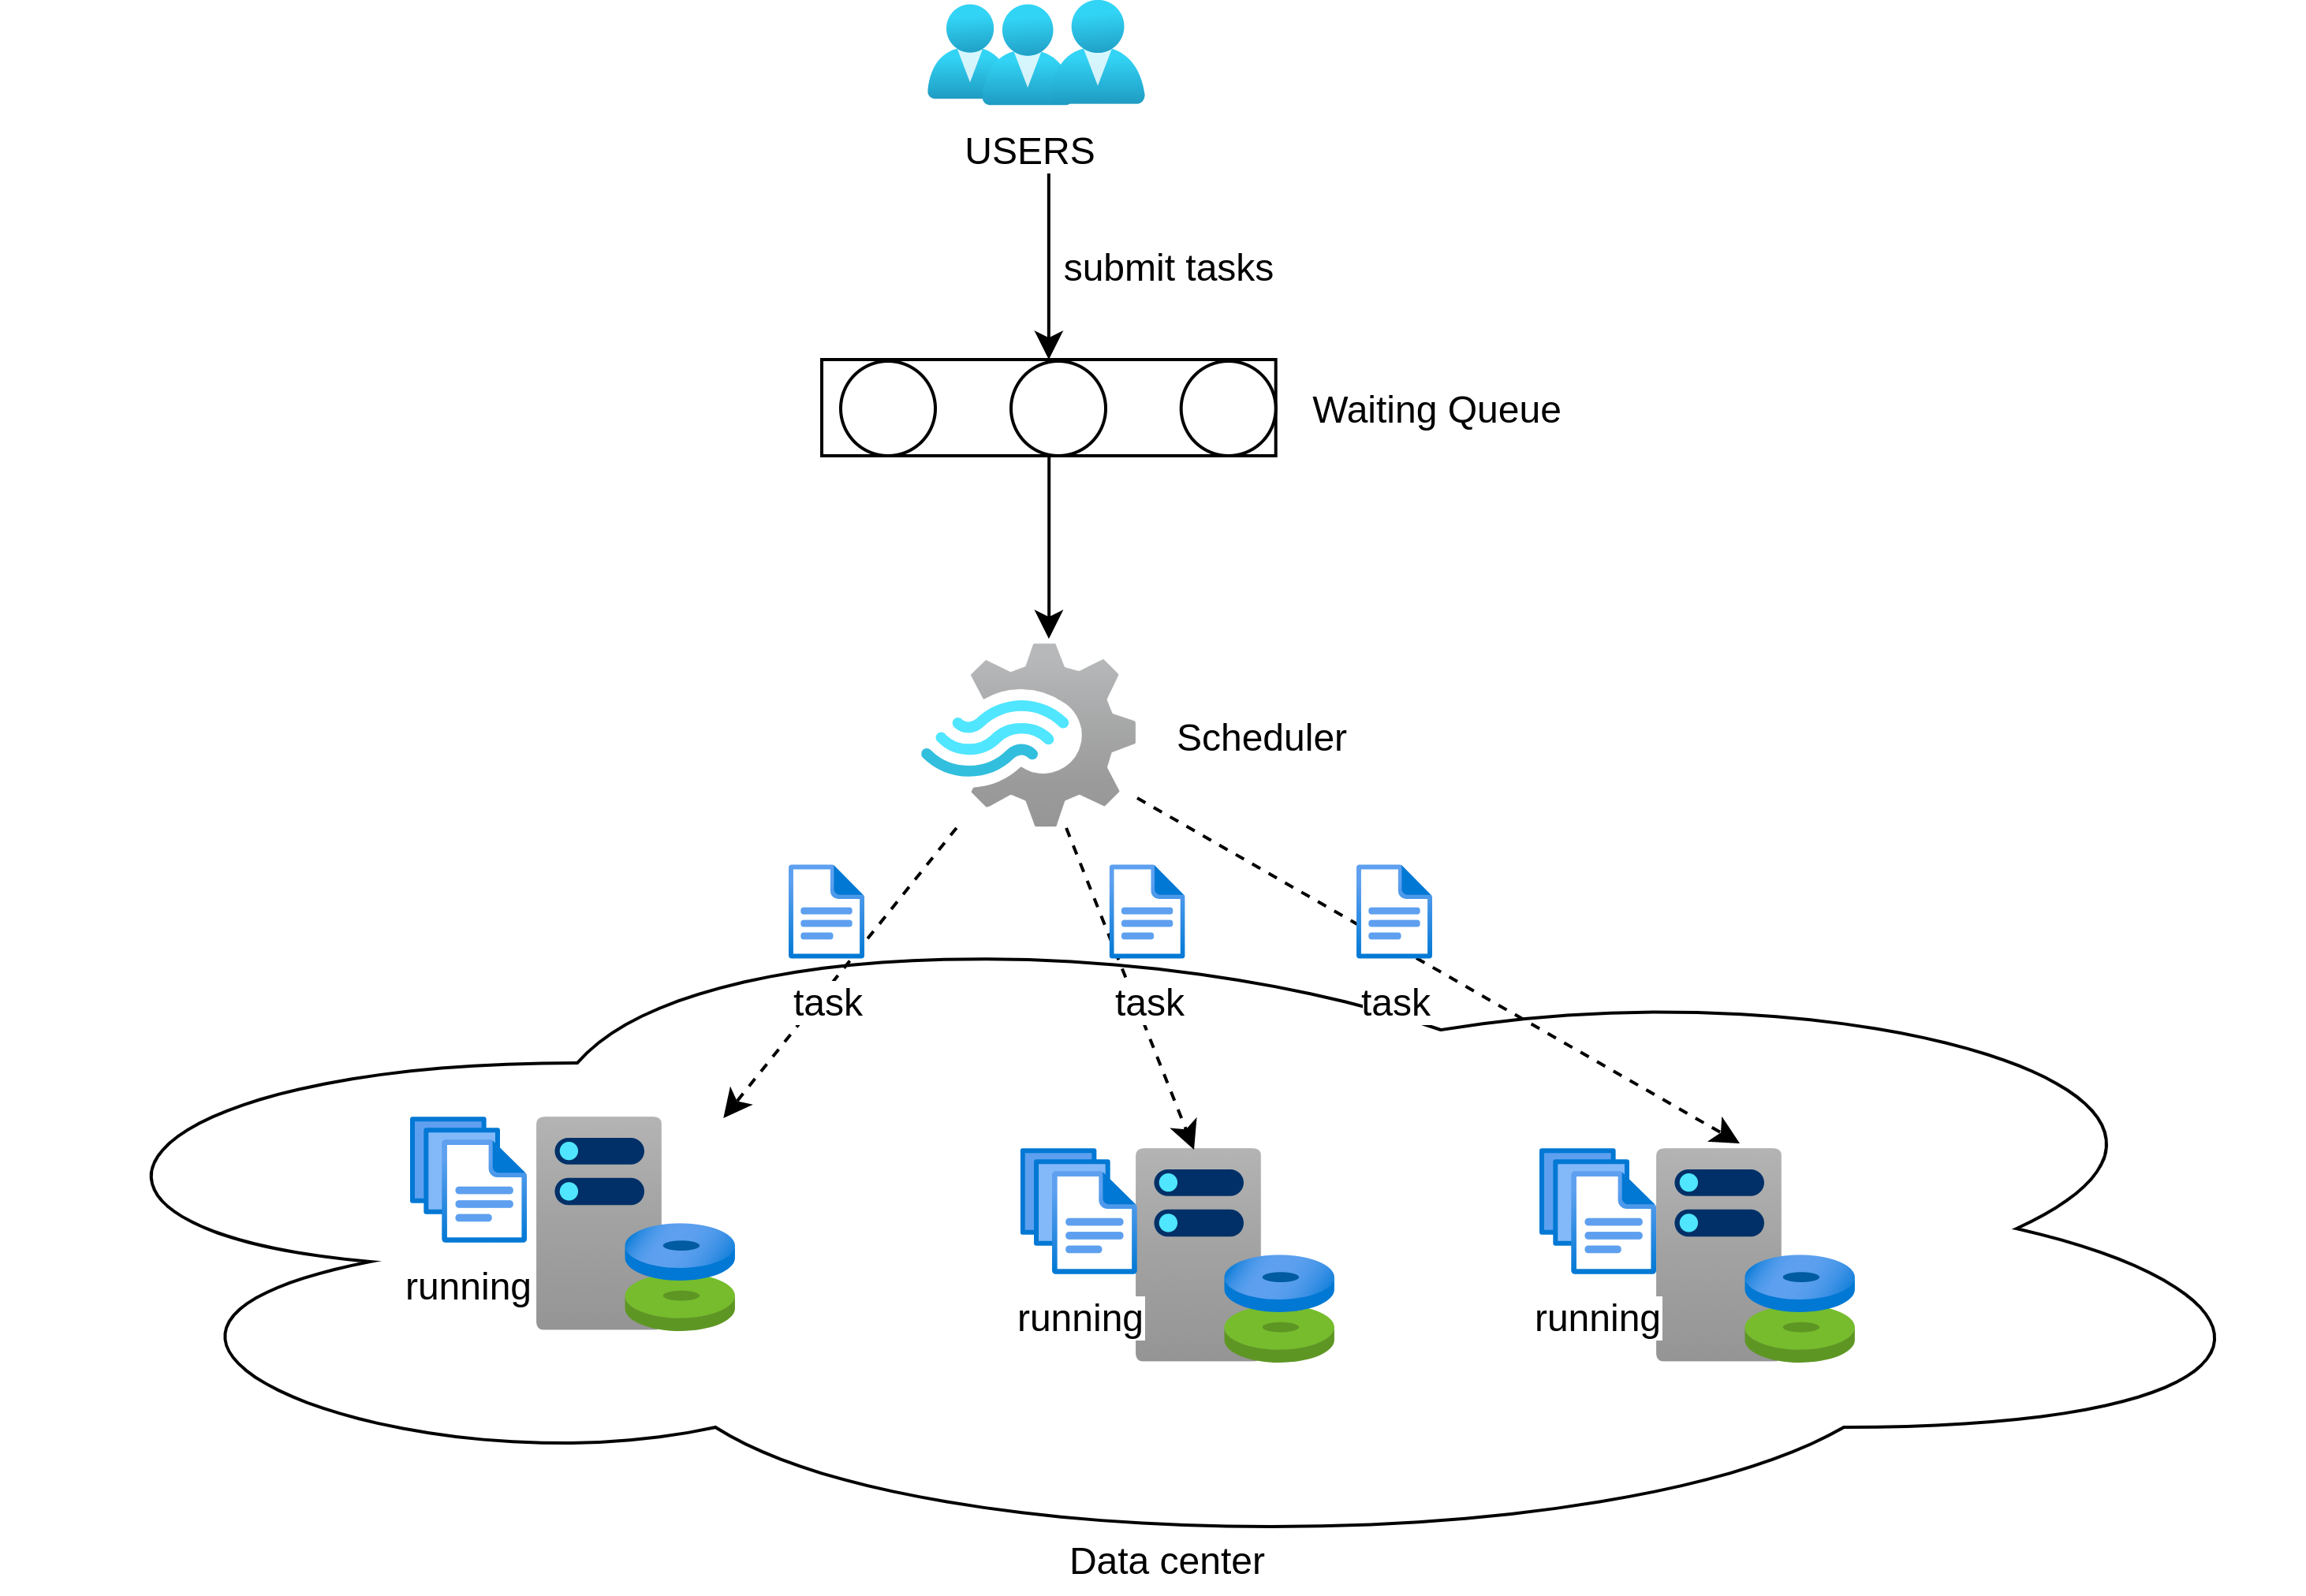
\includegraphics[scale=0.4]{images/basic_flow.png}
		\caption{Người dùng gửi tasks đến hệ thống}
	\end{figure}
\end{minipage}
\end{frame}

\begin{frame}
{Vấn đề lập lịch trong hệ thống Cloud}
% Tại sao cần lập lịch trong hệ thống Cloud
\begin{minipage}[t]{0.48\linewidth}
	\vspace{1cm}
	\begin{block}
	{Tại sao cần lập lịch?}
	\begin{enumerate}
		\item Tiết kiệm chi phí nhờ sử dụng hiệu quả tài nguyên 
		\item Tăng chất lượng dịch vụ cung cấp cho người dùng
	\end{enumerate}
	\end{block}
\end{minipage}
\hfill
\begin{minipage}[t]{0.48\linewidth}
	\begin{figure}
		\centering
		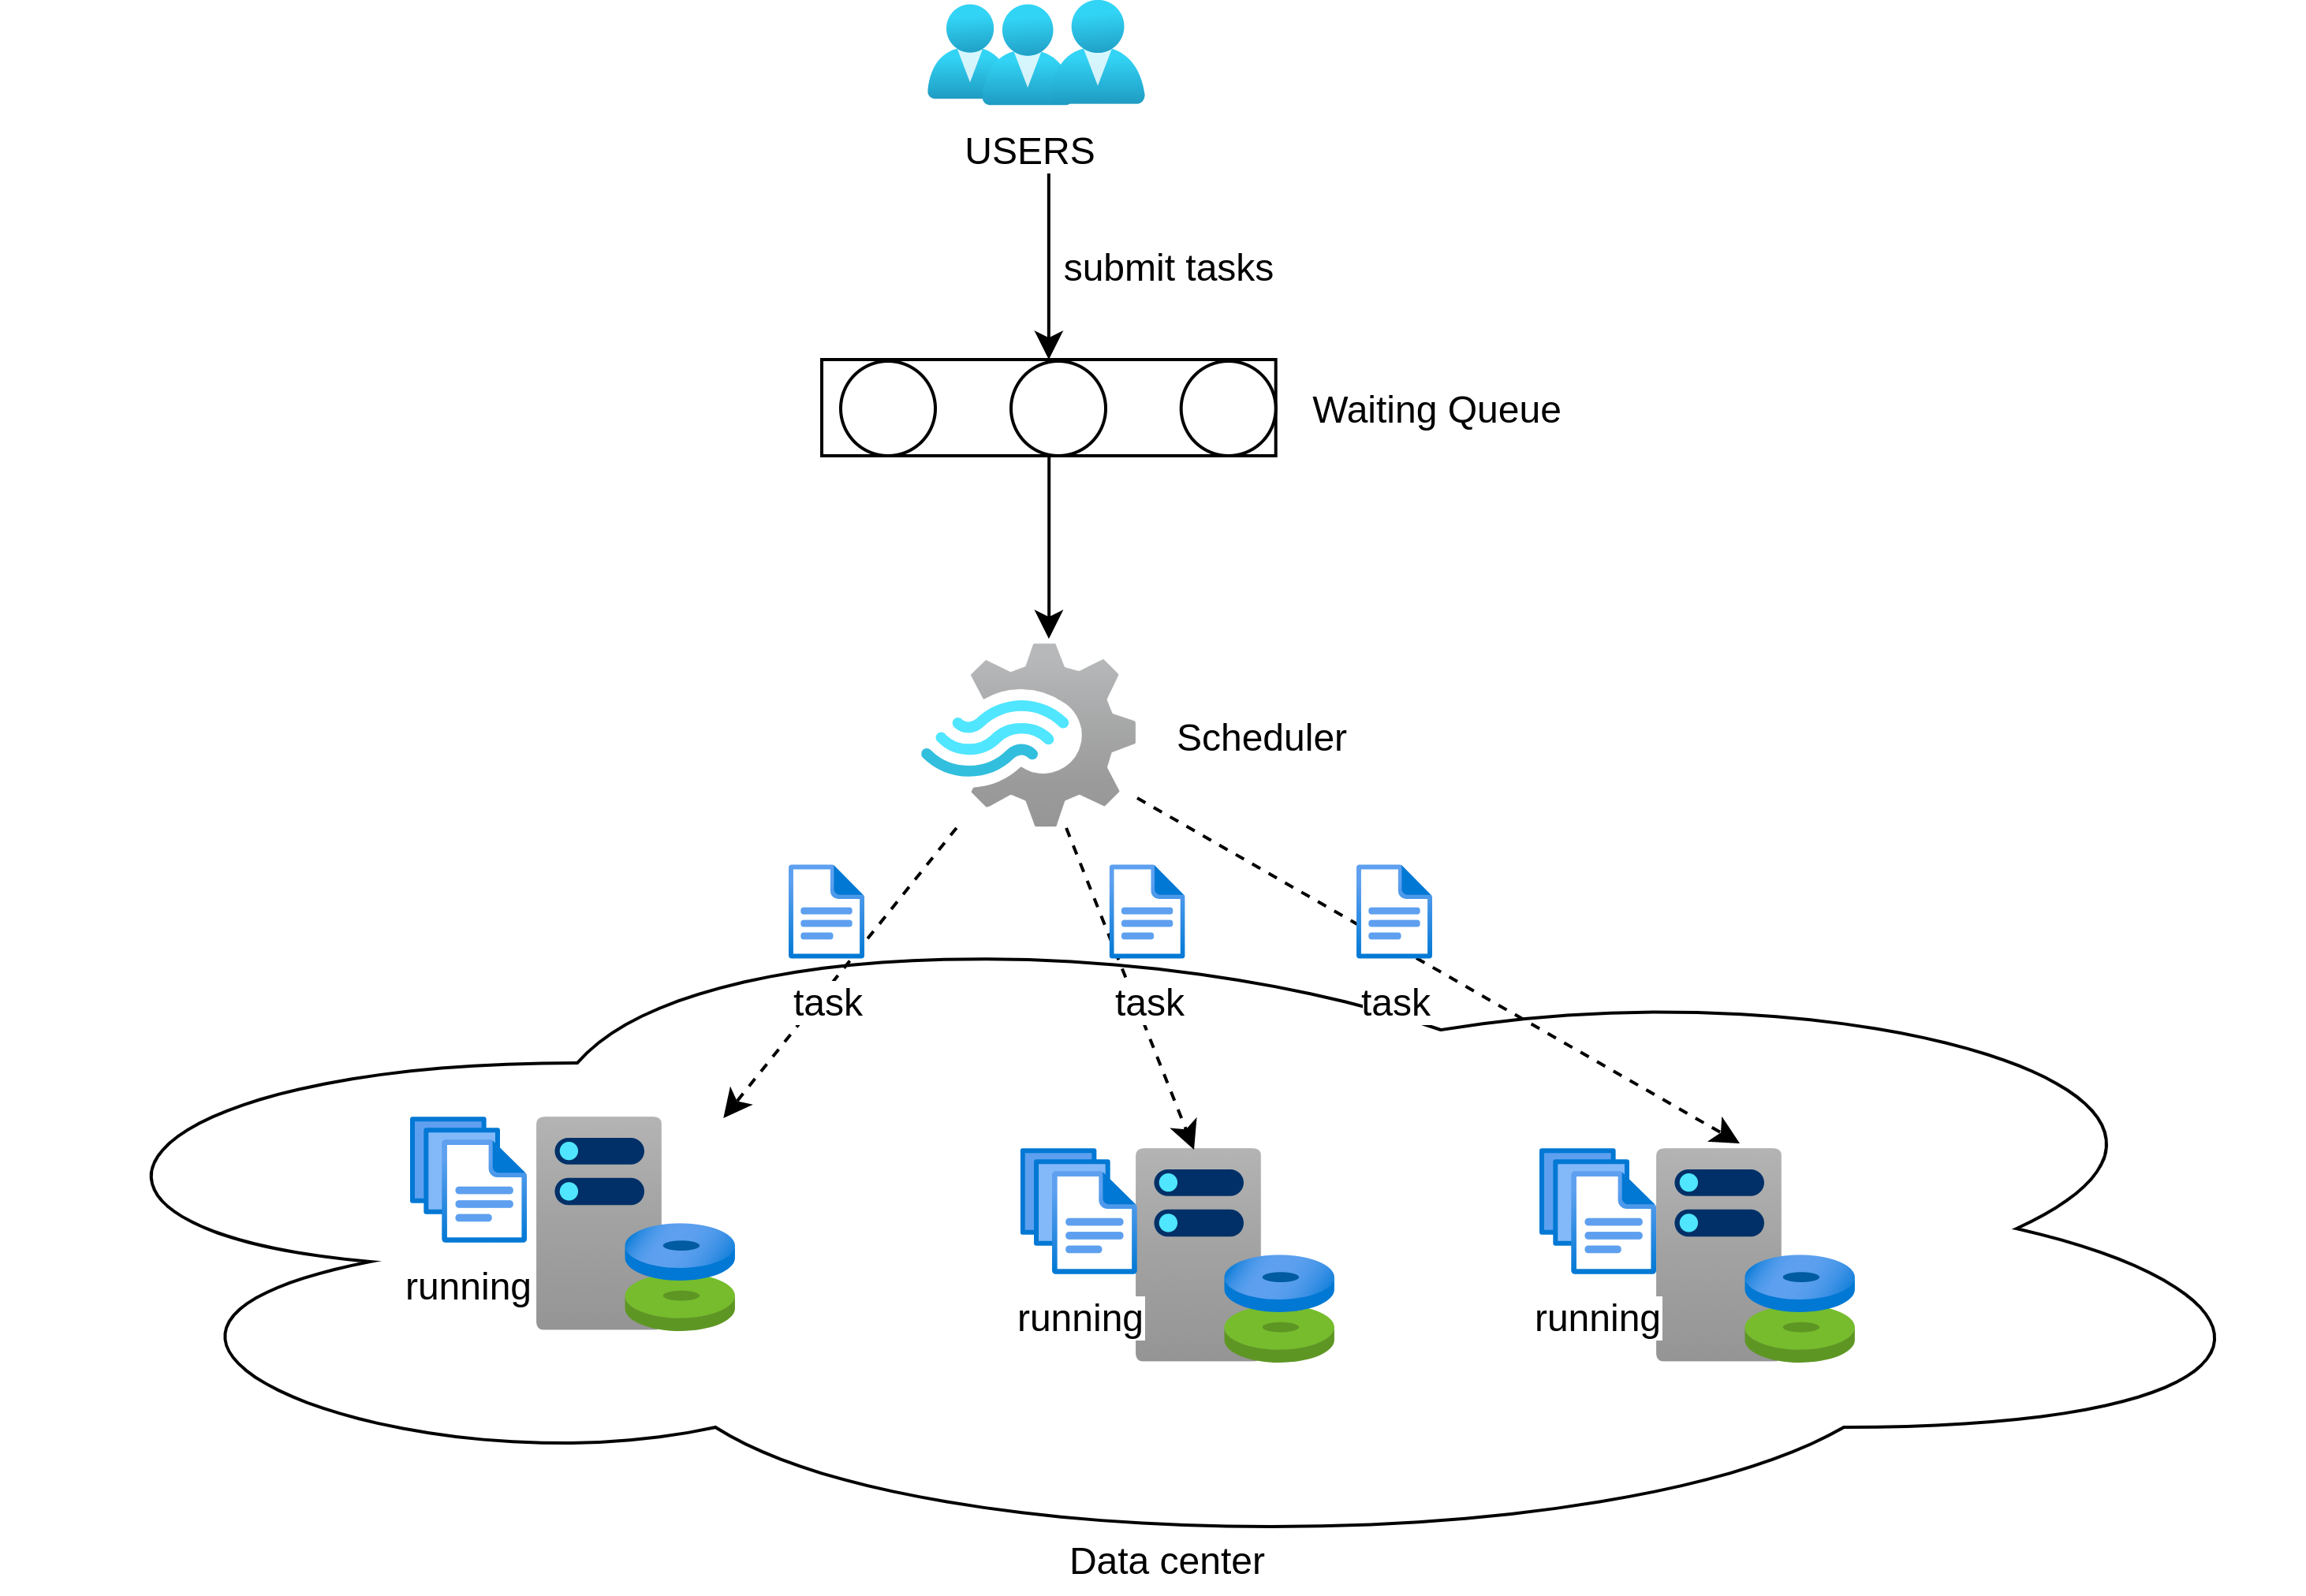
\includegraphics[scale=0.4]{images/basic_flow.png}
		\caption{Người dùng gửi tasks đến hệ thống}
	\end{figure}
\end{minipage}
\end{frame}

%\begin{frame}
%{Các dạng lập lịch}
%\begin{block}
%{Hai kiểu lời giải phổ biển cho bài toán}
%\begin{itemize}
%	\item Có N tasks, M máy ảo, lời giải là cách ghép cặp task -> máy ảo cho N tasks. 
%	\item Có K nhóm của tasks, M máy ảo, lời giải là cách phân chia 
%		\[
%			\Theta = \{\theta_{1}, ..., \theta_{K}\}
%		\]
%		với \begin{itemize}
%			\item $\theta_{i}$ là số lượng máy tính ảo được phân cho nhóm i 
%			\item $\sum_{i = 1}^{K}\theta_{i} = M$
%		\end{itemize}
%\end{itemize}
%\end{block}
%\end{frame}

\begin{frame}
{Các thuật toán phổ biển}
\begin{block}
{Heuristic}
Là những thuật toán đưa ra lời giải chấp nhận được, thỏa mãn mục tiêu và ràng buộc của bài toán 
\begin{itemize}
	\item Nhóm các thuật toán dựa trên quần thể như GA, PSO, ...
	\item Nhóm các thuật toán tìm kiếm lời giải tối ưu như Tabu Search, Beam Search
\end{itemize} 
\end{block}
\begin{block}
{Đặc điểm chung}
\begin{itemize}
	\item Tìm nghiệm tối ưu hàm $\mathcal{F}$ nào đó trong miền không gian có ràng buộc
	\item Hàm $\mathcal{F}$ sẽ được tính dựa trên các thông tin về hệ thống tại thời điểm lập lịch
\end{itemize}
\end{block}
\end{frame}

\section{Các vấn đề của bài toán lập lịch thời gian thực}

\begin{frame}
{Sai số do độ trễ trong quá trình lập lịch}
% Vấn đề và nguồn gốc của sự sai số 
	\begin{minipage}[t]{0.4\linewidth}
		\begin{block}{Trạng thái tài nguyên}
		\begin{itemize}
			\item Tại thời điểm $t_{1}$
			\begin{itemize}
				\item available\_cpu = $c_{1}$
				\item available\_memory = $m_{1}$
			\end{itemize}
			\item  Tại thời điểm $t_{2}$
			\begin{itemize}
				\item available\_cpu = $c_{2}$
				\item available\_memory = $m_{2}$
			\end{itemize}
		\end{itemize}
		\end{block}
	\end{minipage}
	\hfill
	\begin{minipage}[t]{0.59\linewidth}
		\begin{figure}
			\centering
			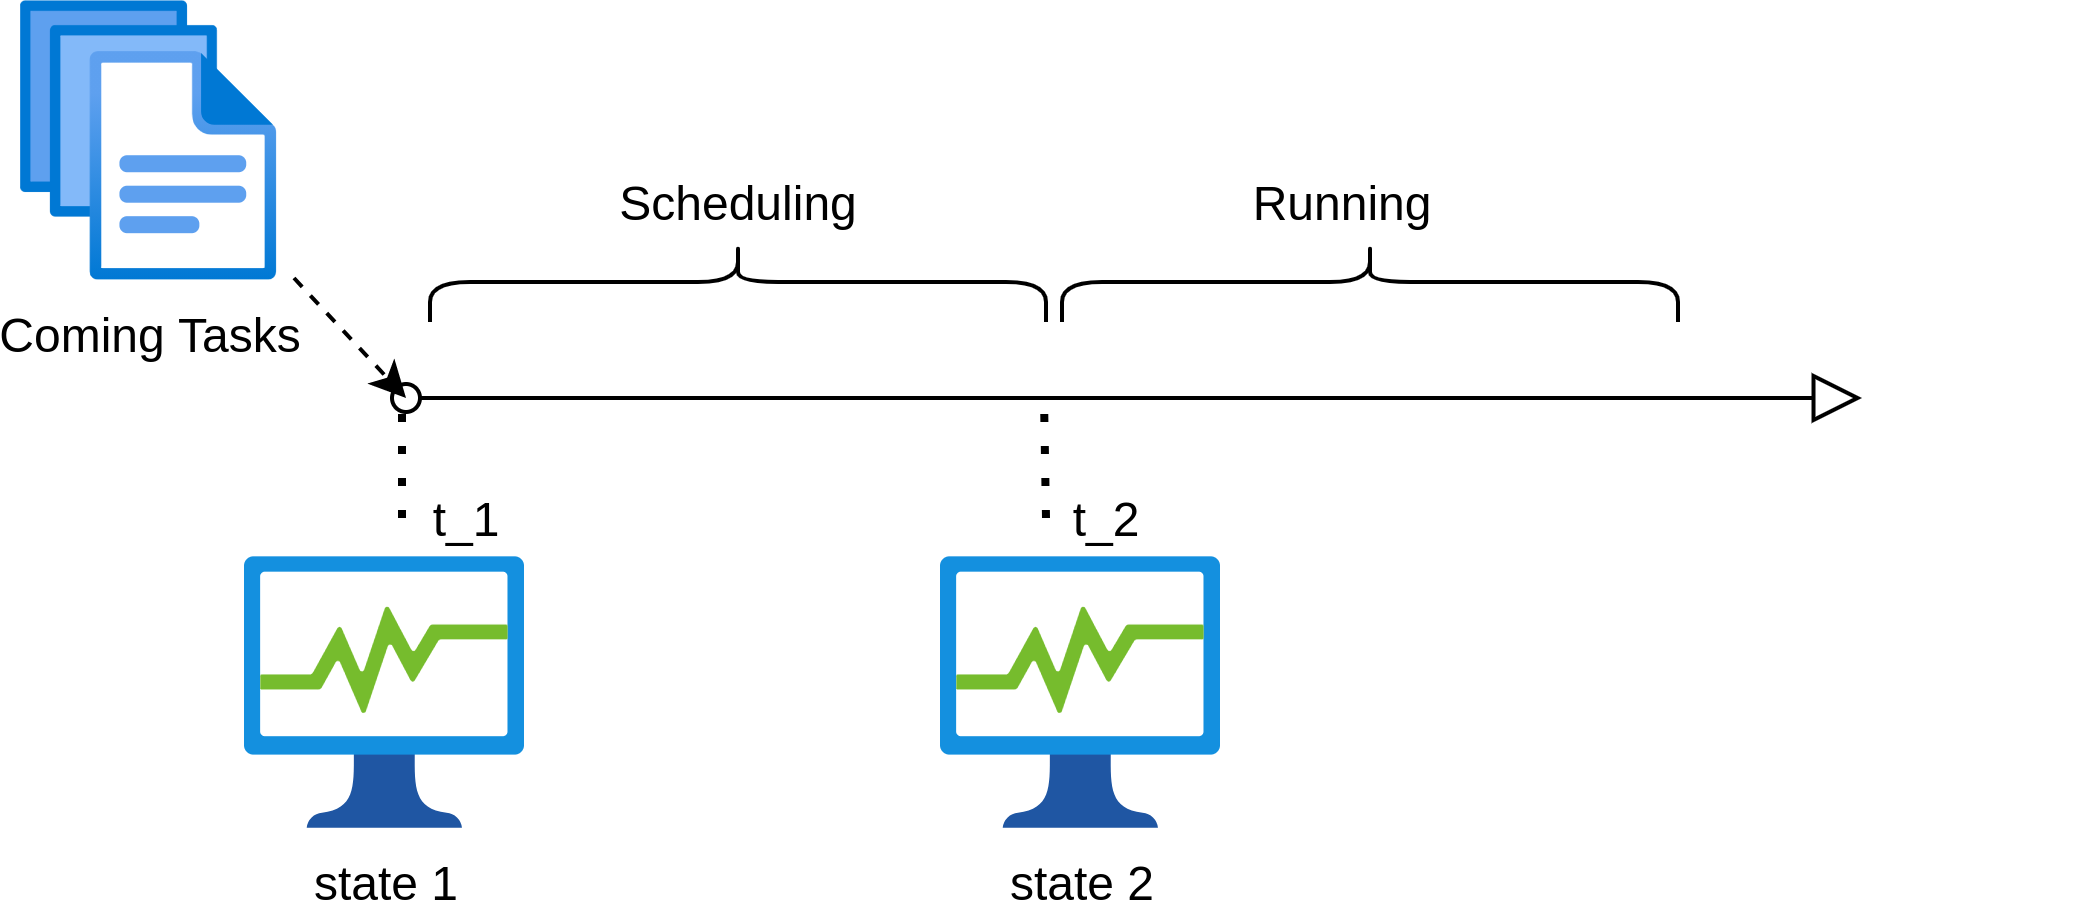
\includegraphics[scale=0.5]{images/state_change.png}
			\caption{Trạng thái máy tính}
		\end{figure}
	\end{minipage}
	\pause
	\begin{center}
		\begin{block}
		{\centering Vấn đề 1}
				\centering $c_{1} \neq c_{2}$ hoặc $m_{1} \neq m_{2}$ làm mất sự tối ưu của nghiệm thuật toán lập lịch 
		\end{block}
	\end{center}
\end{frame}

%\begin{frame}
%{Ảnh hưởng của thời gian lập lịch}
%\begin{figure}
%\centering
%\begin{subfigure}{.5\textwidth}
%  \centering
%  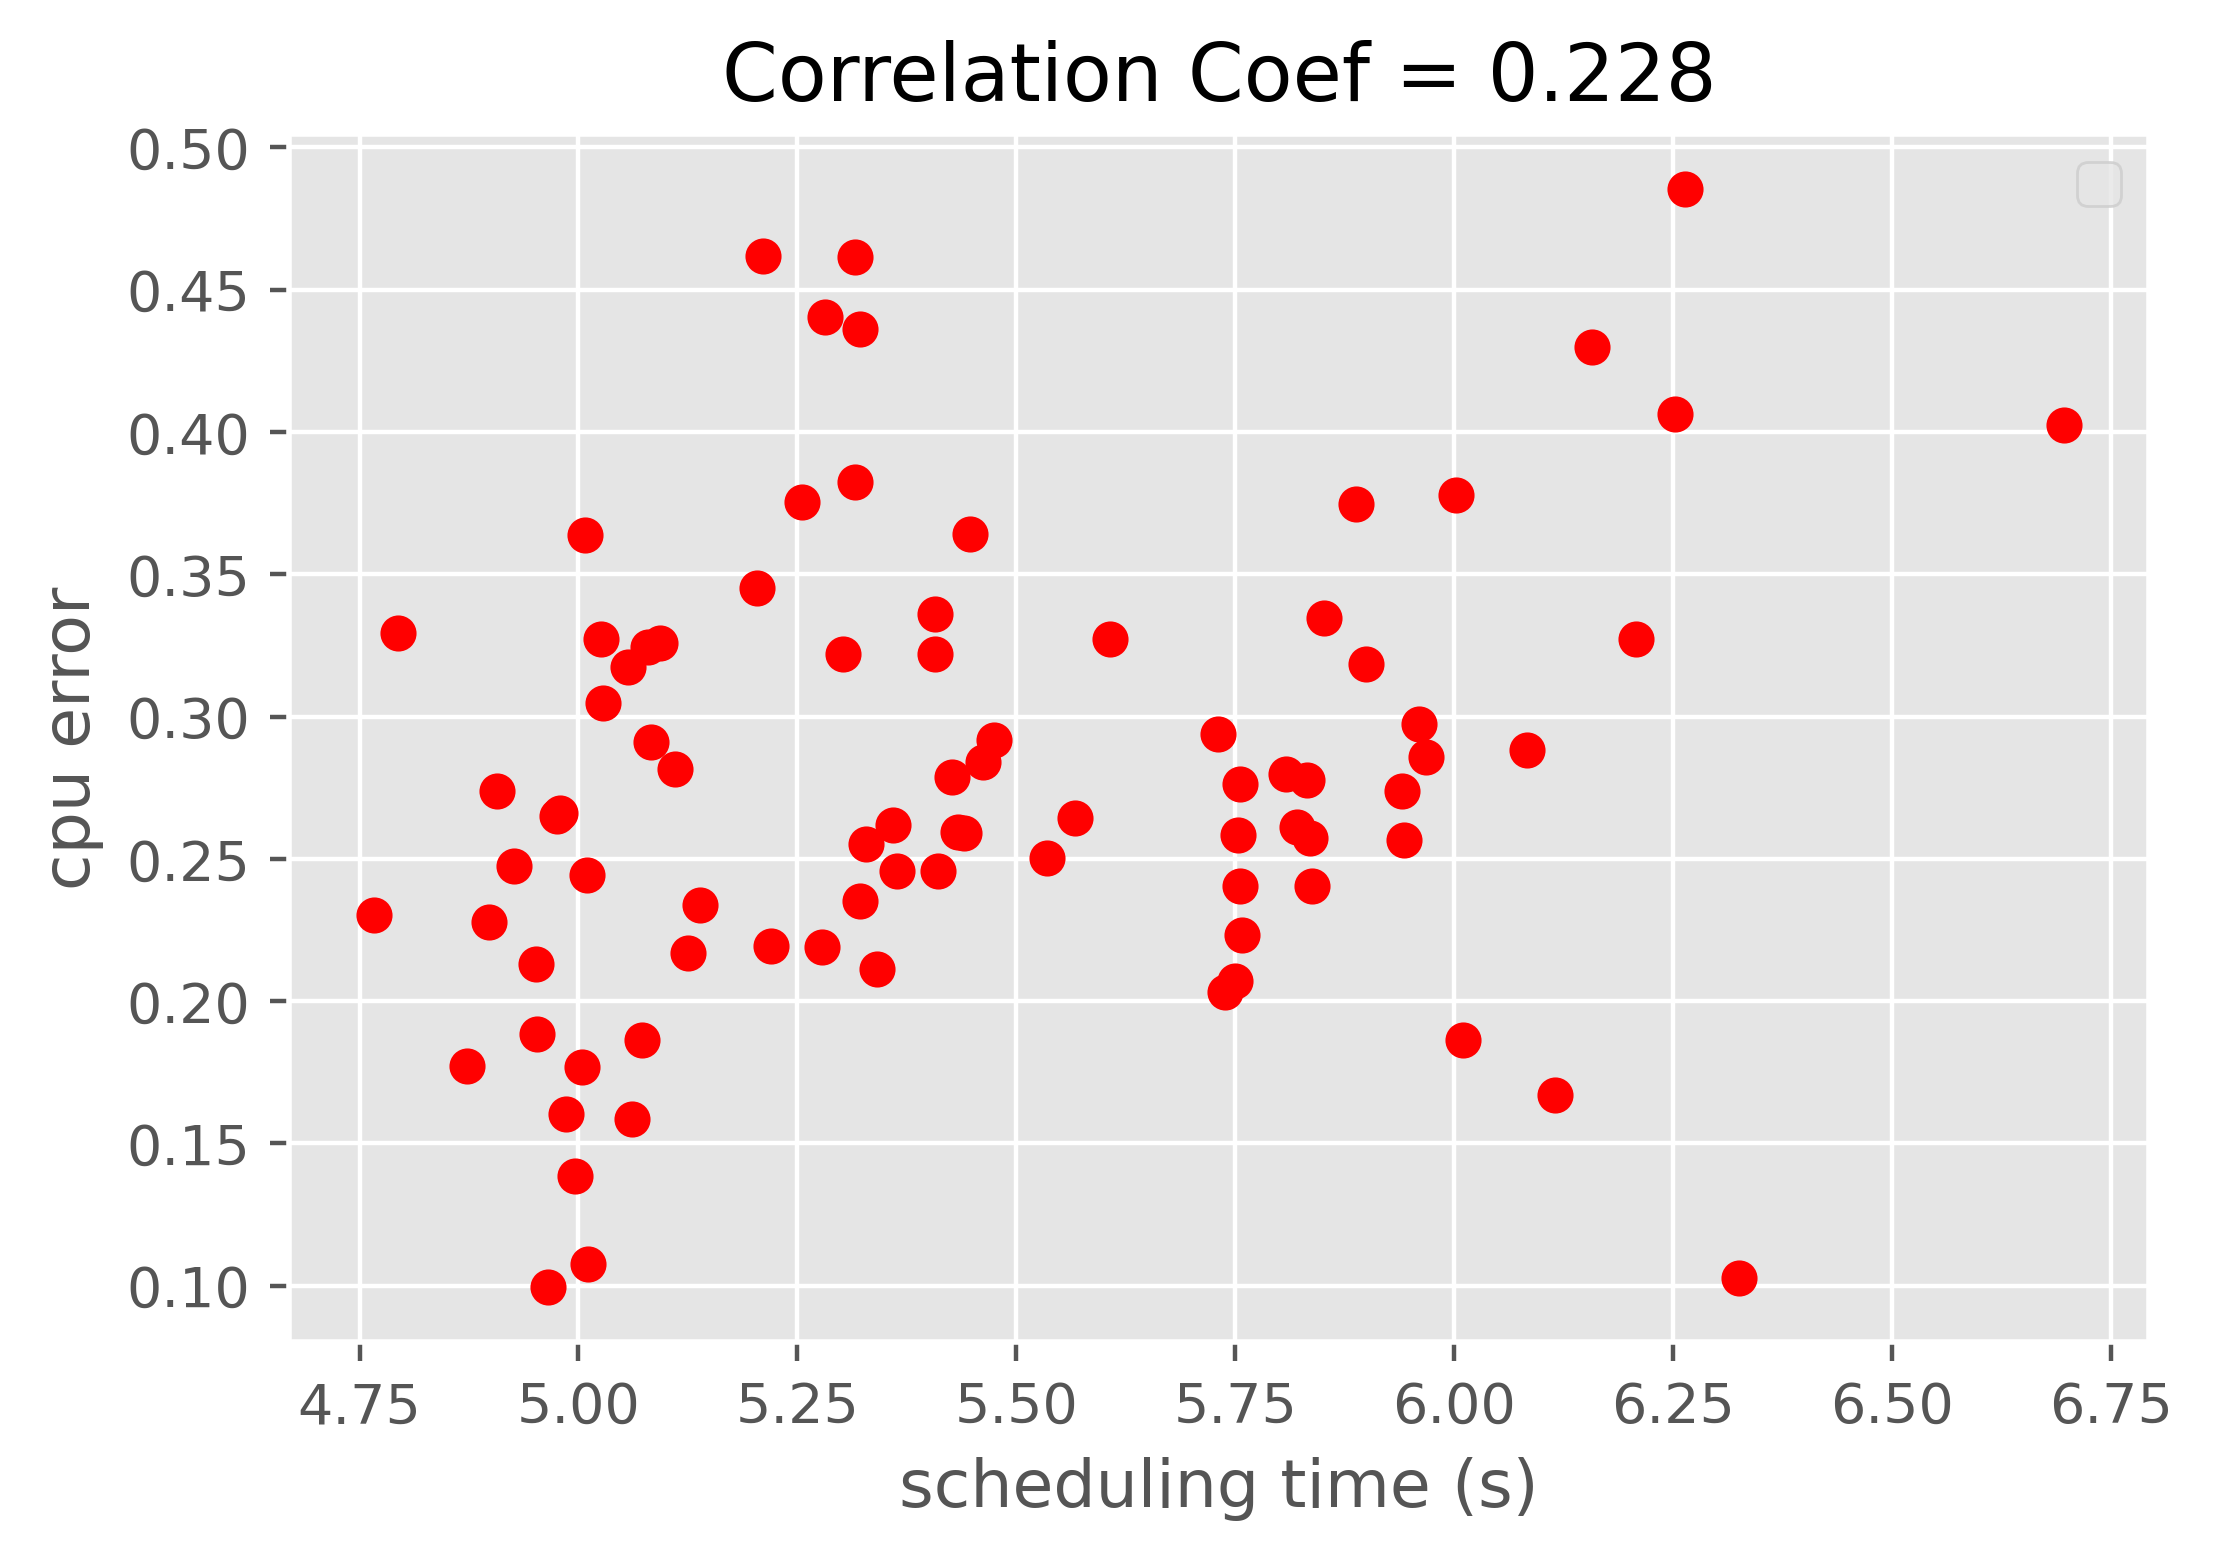
\includegraphics[width=.85\linewidth]{images/scheduling_time_vs_delta.png}
%  \caption{Thời gian trễ với độ lệch số liệu}
%\end{subfigure}%
%\begin{subfigure}{.5\textwidth}
%  \centering
%  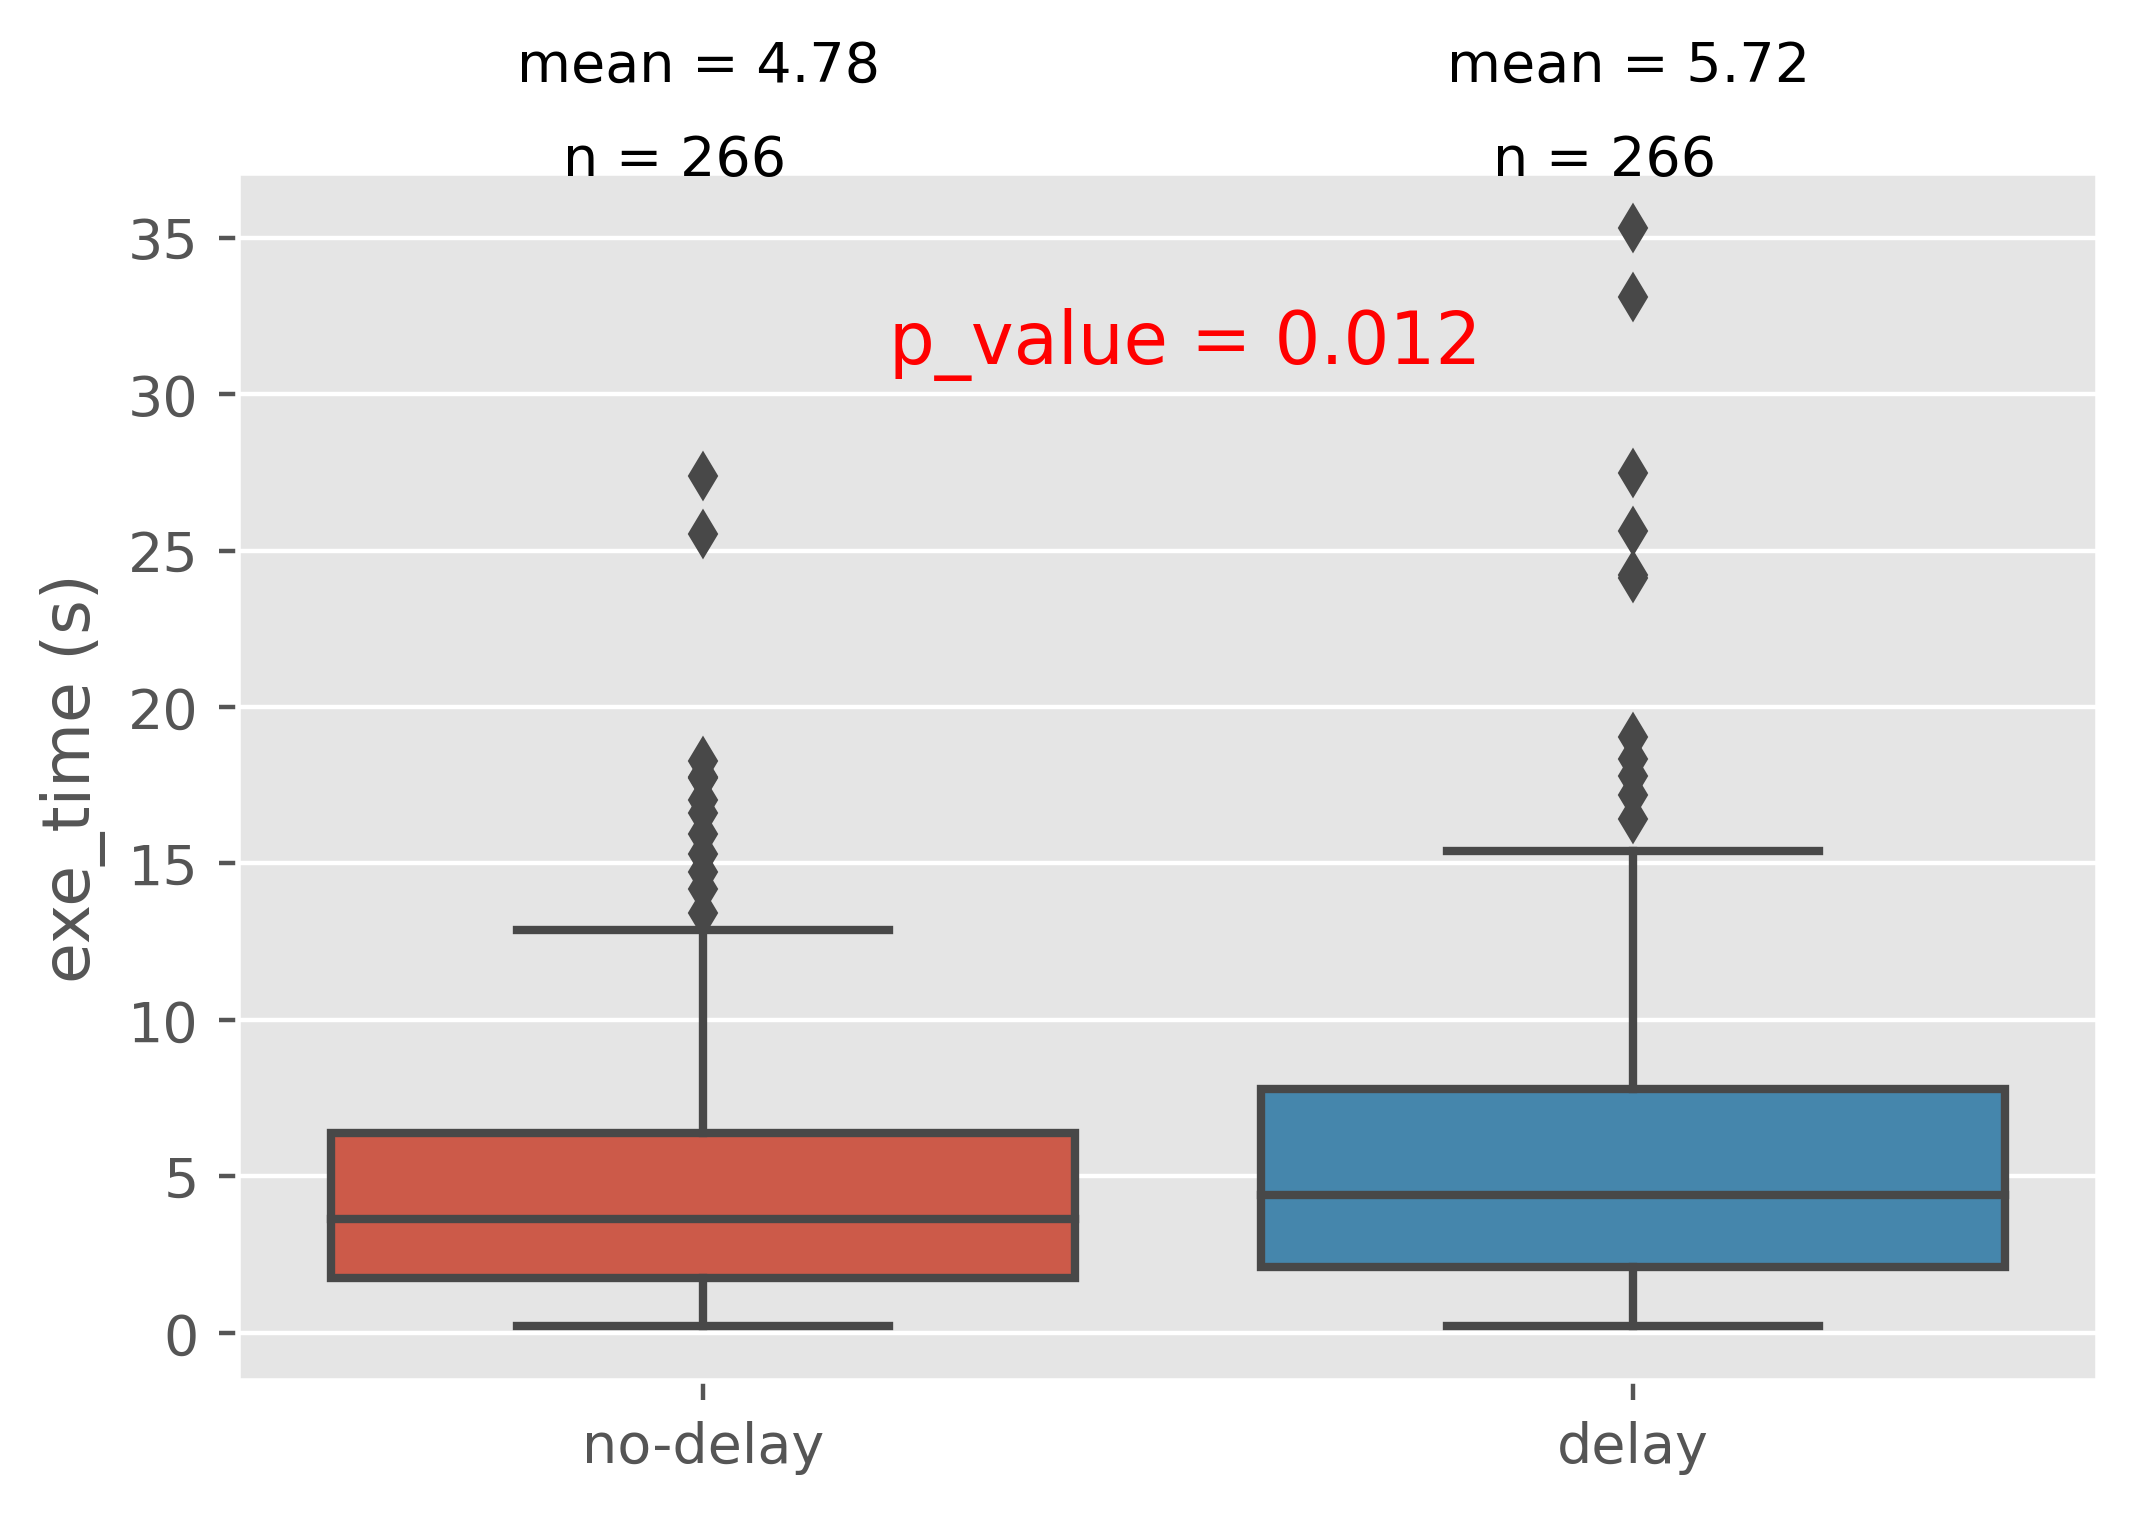
\includegraphics[width=.9\linewidth]{images/delay_impact.png}
%  \caption{Sự trễ làm tăng thời gian thực thi}
%\end{subfigure}
%\caption{Thông số tại thời điểm kết thúc lập lịch}
%\label{fig:usage_est}
%\end{figure}
%\end{frame}


\begin{frame}
{Mất cân bằng khối lượng công việc khi hoạt động}

\begin{minipage}[t]{0.34\linewidth}
	\begin{itemize}
		\item long-run: các tasks dạng service luôn luôn chạy 
		\item batch-job: các tasks thuộc dạng batch, thời gian thực thi từ vài trăm mili giây tới vài giây 
	\end{itemize}
\end{minipage}
\hfill
\begin{minipage}[t]{0.65\linewidth}
\begin{figure}
	\centering
	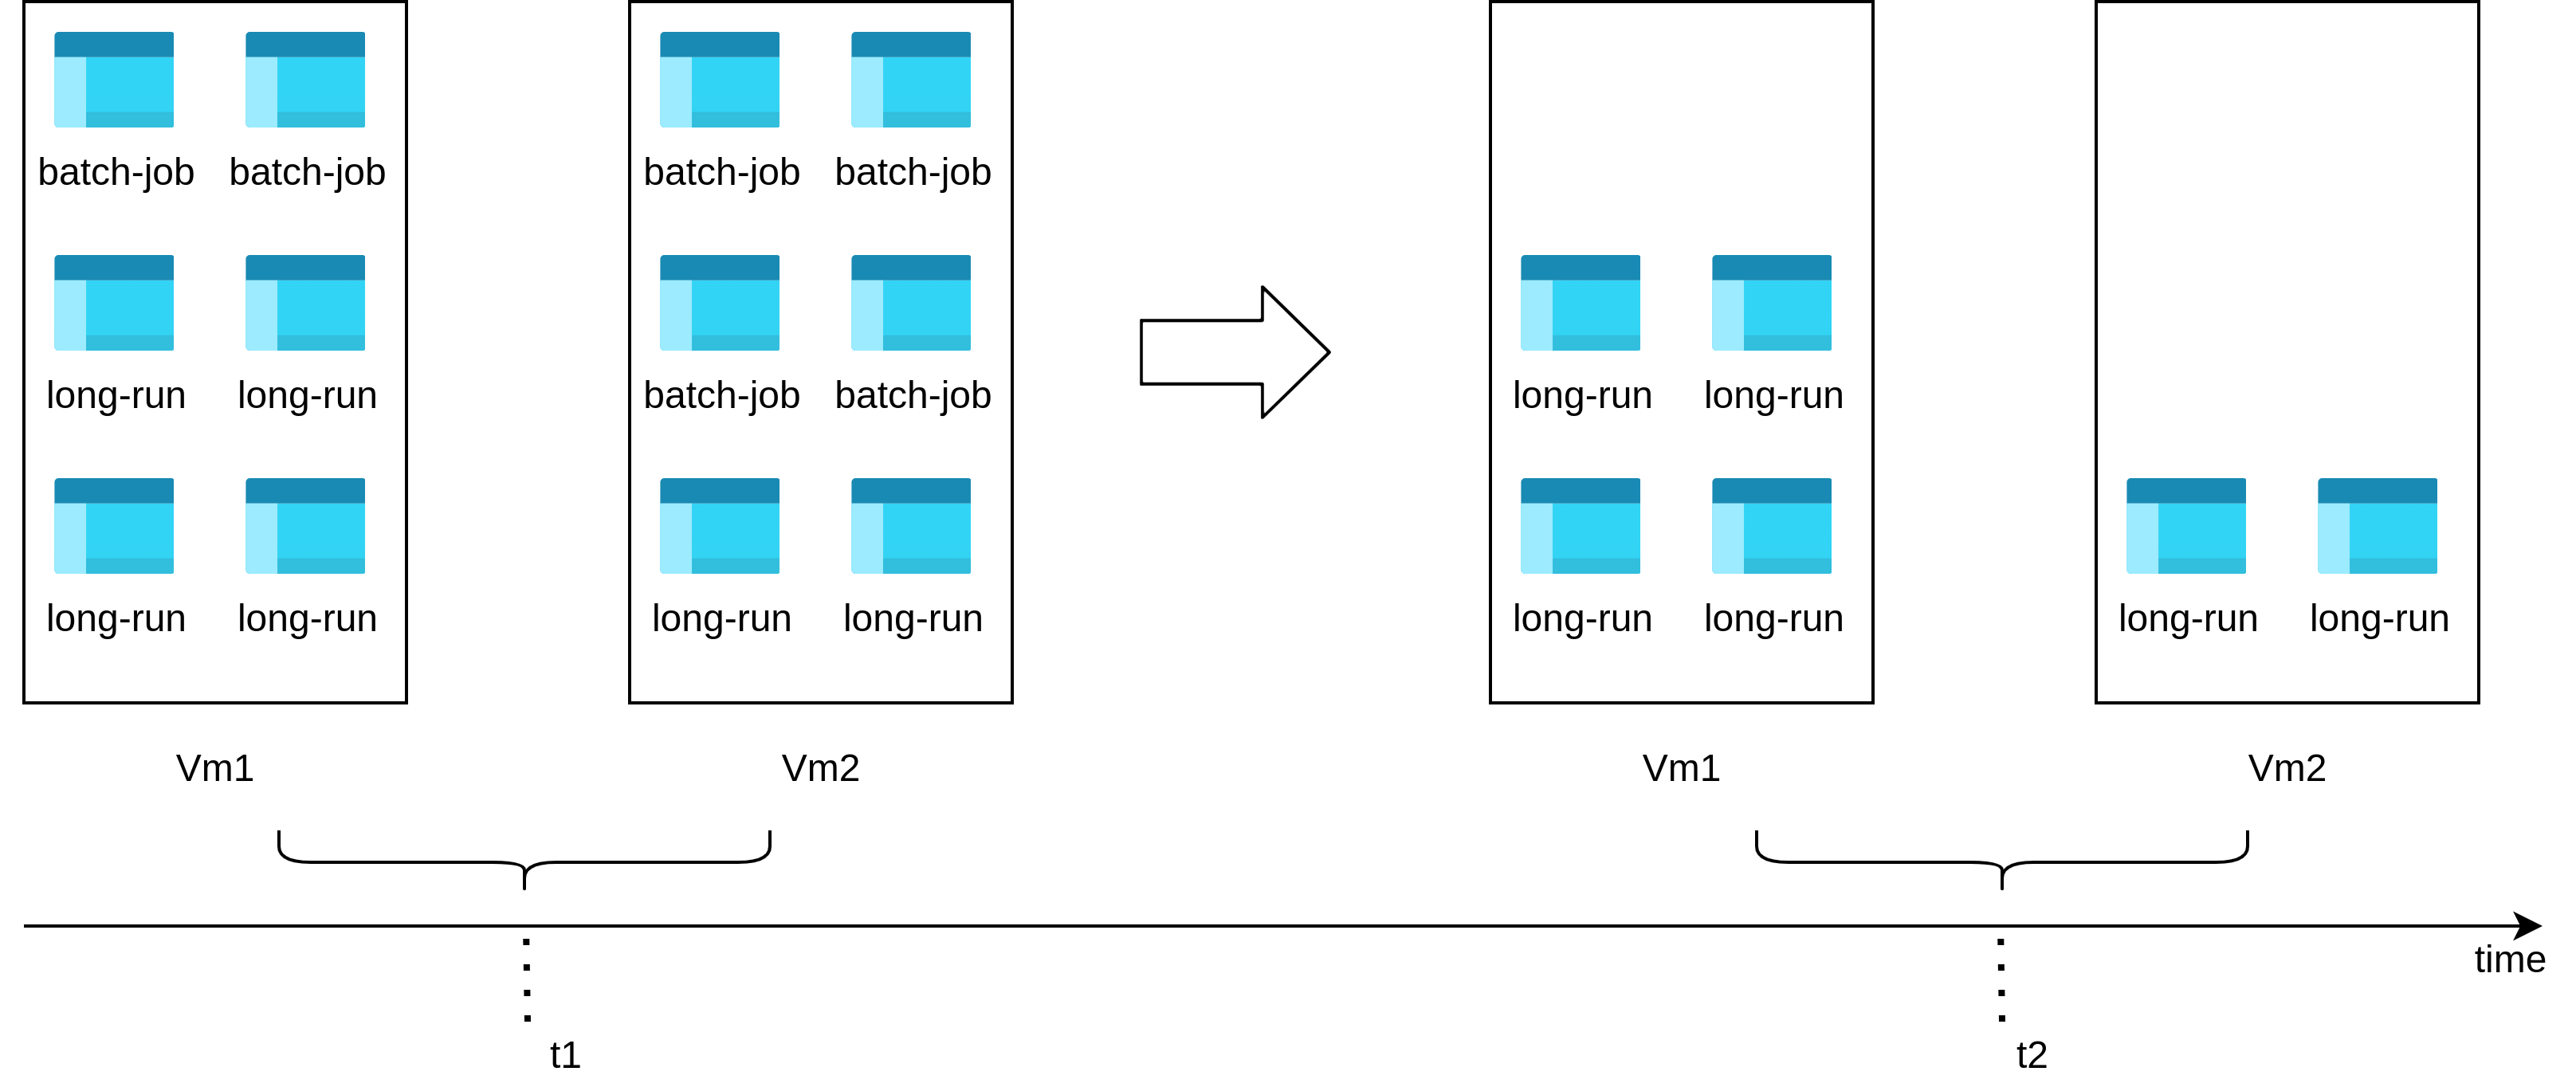
\includegraphics[scale=0.35]{images/unload_balancing.png}
	\caption{Mất cân bằng khối lượng tasks}
	\label{fig:unload_balancing}
\end{figure}
\end{minipage}
\pause
	\begin{block}
	{\centering Vấn đề 2}
		\centering Các batch-job tasks kết thúc trong quá trình chạy phá vỡ trạng thái cân bằng khối lượng công việc giữa các máy ảo 
	\end{block}
% Hiện tượng mất cân bằng khối lượng các máy trong quá trình chạy, nguyên nhân 
\end{frame}


%\section{Mục tiêu đồ án}
%\begin{frame}
%{Mục tiêu của đồ án nghiên cứu}
%% Đưa ra mục tiêu nghiên cứu bao gồm xác định các nguyên nhân của các vấn đề trên và đưa ra giải pháp cải thiện
%\pause 
%\begin{block}
%{Dự đoán tài nguyên tại thời điểm thực thi}
%\pause
%Dùng mạng Bayesian dự đoán trạng thái tasks trong hệ thống tại thời điểm kết thúc lập lịch
%\end{block}
%\pause
%\begin{block}
%{Giảm sự mất cân bằng khối lượng tasks trong thời gian hoạt động}
%\pause 
%Cân bằng khối lượng tasks dài và ngắn giữa các máy tính ảo 
%\end{block}
%\end{frame}

\section{Giải pháp} 

\begin{frame}
{Ước lượng trạng thái các tasks}
\begin{figure}
	\centering
	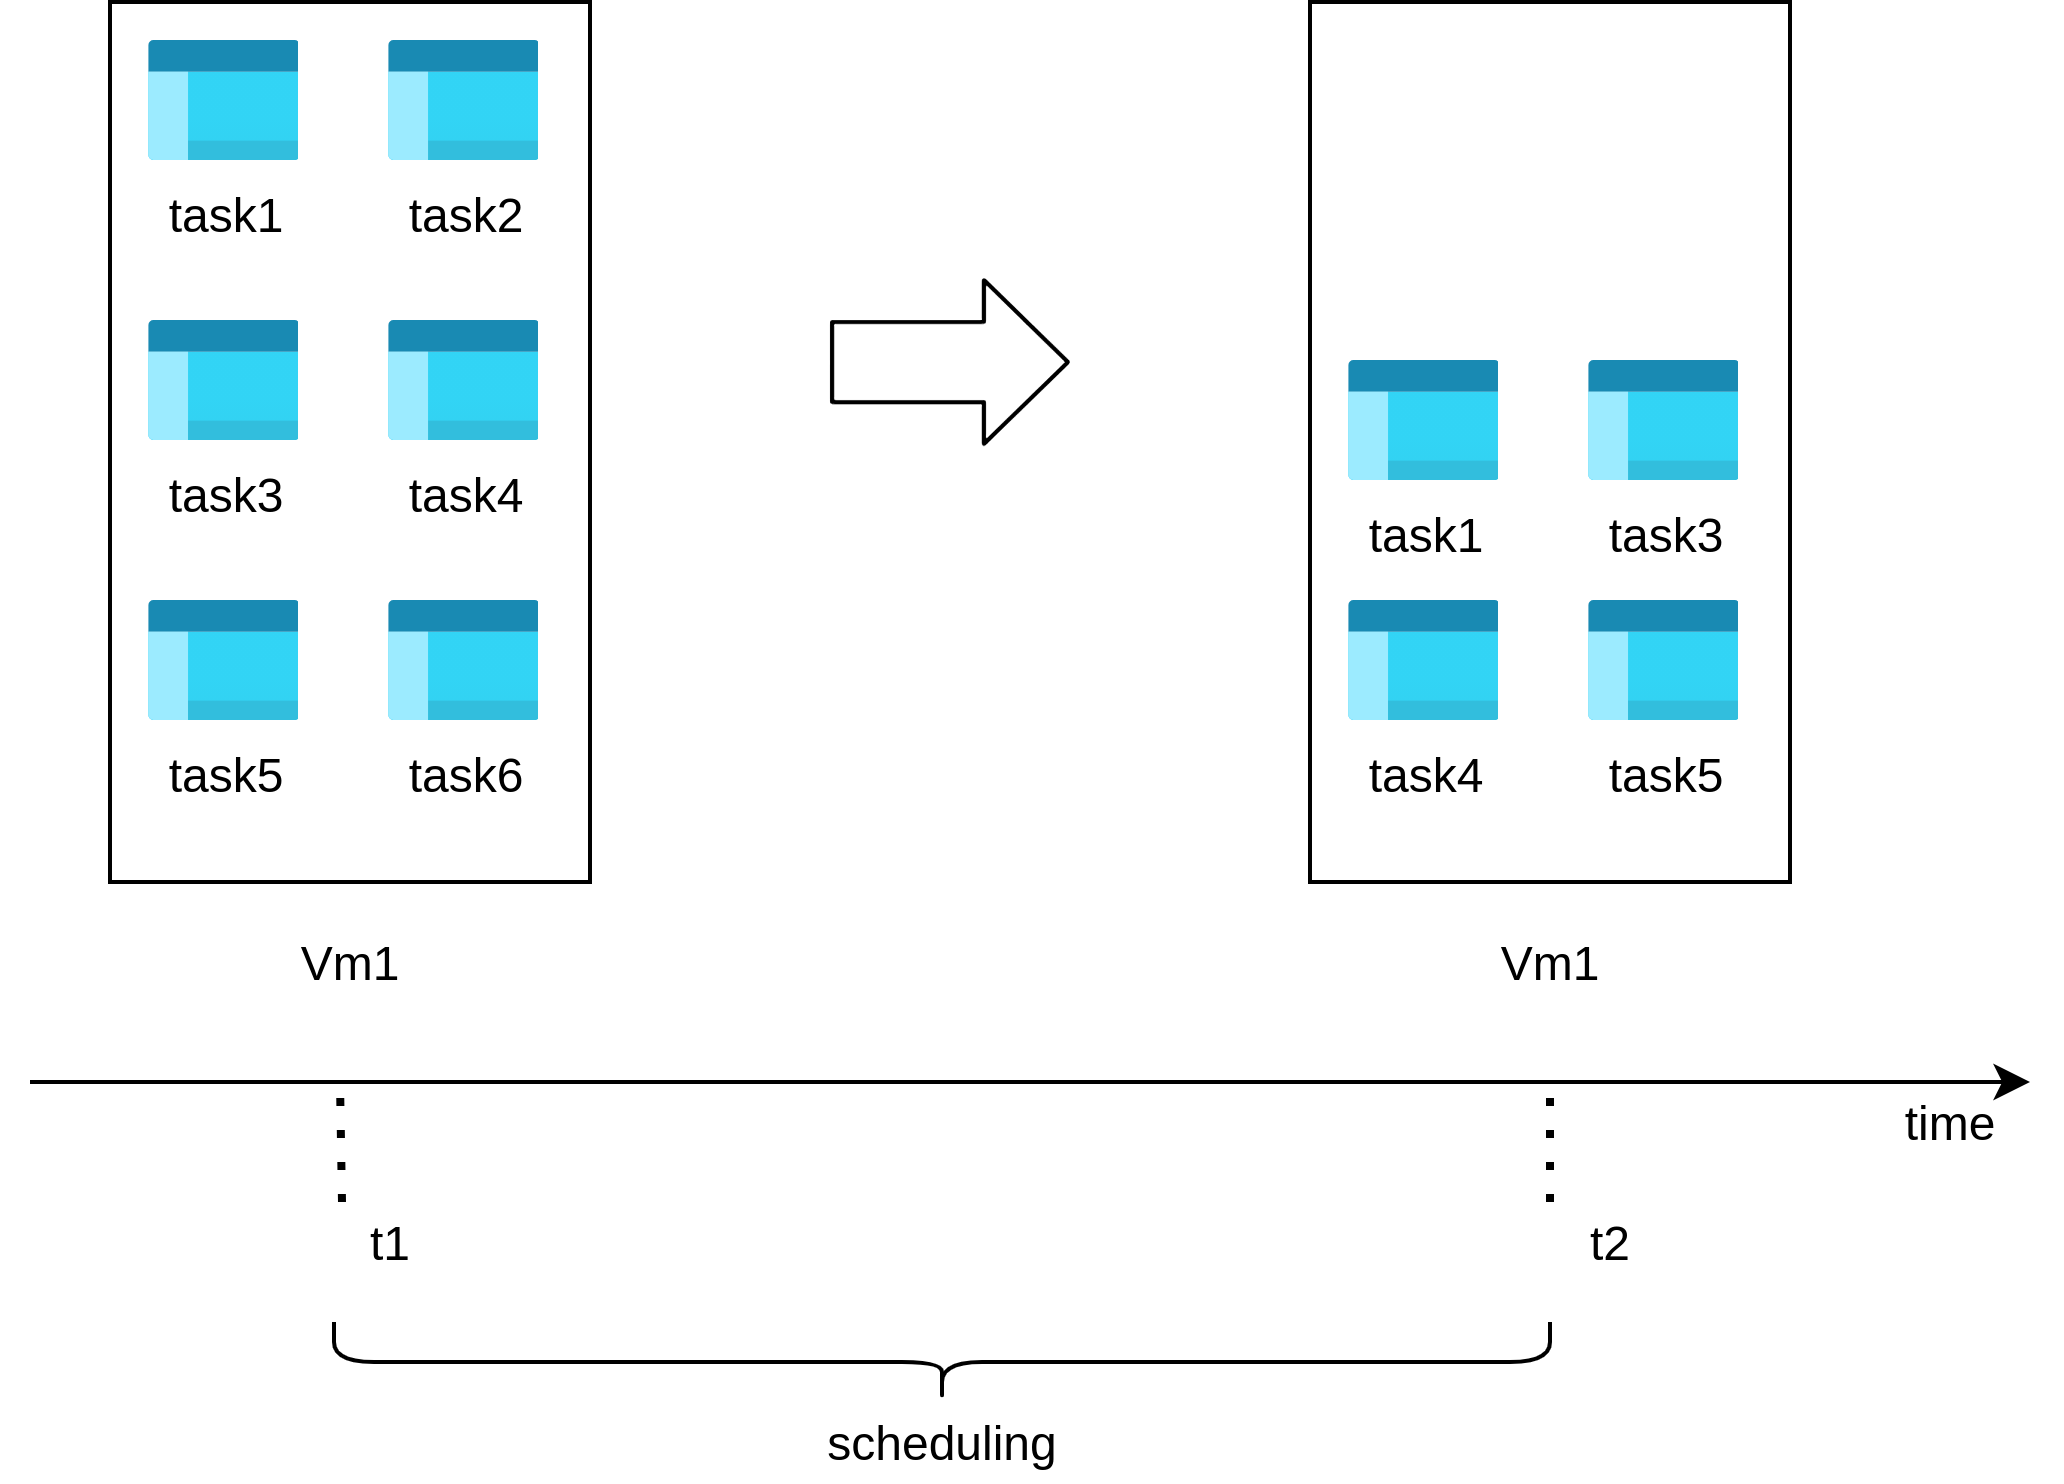
\includegraphics[scale=0.5]{images/predicting_status1.png}
	\caption{Trạng thái tài nguyên tại thời điểm lập lịch và thực thi}
\end{figure}
\end{frame}

%\begin{frame}
%{Ước lượng trạng thái các tasks}
%\begin{figure}
%	\centering
%	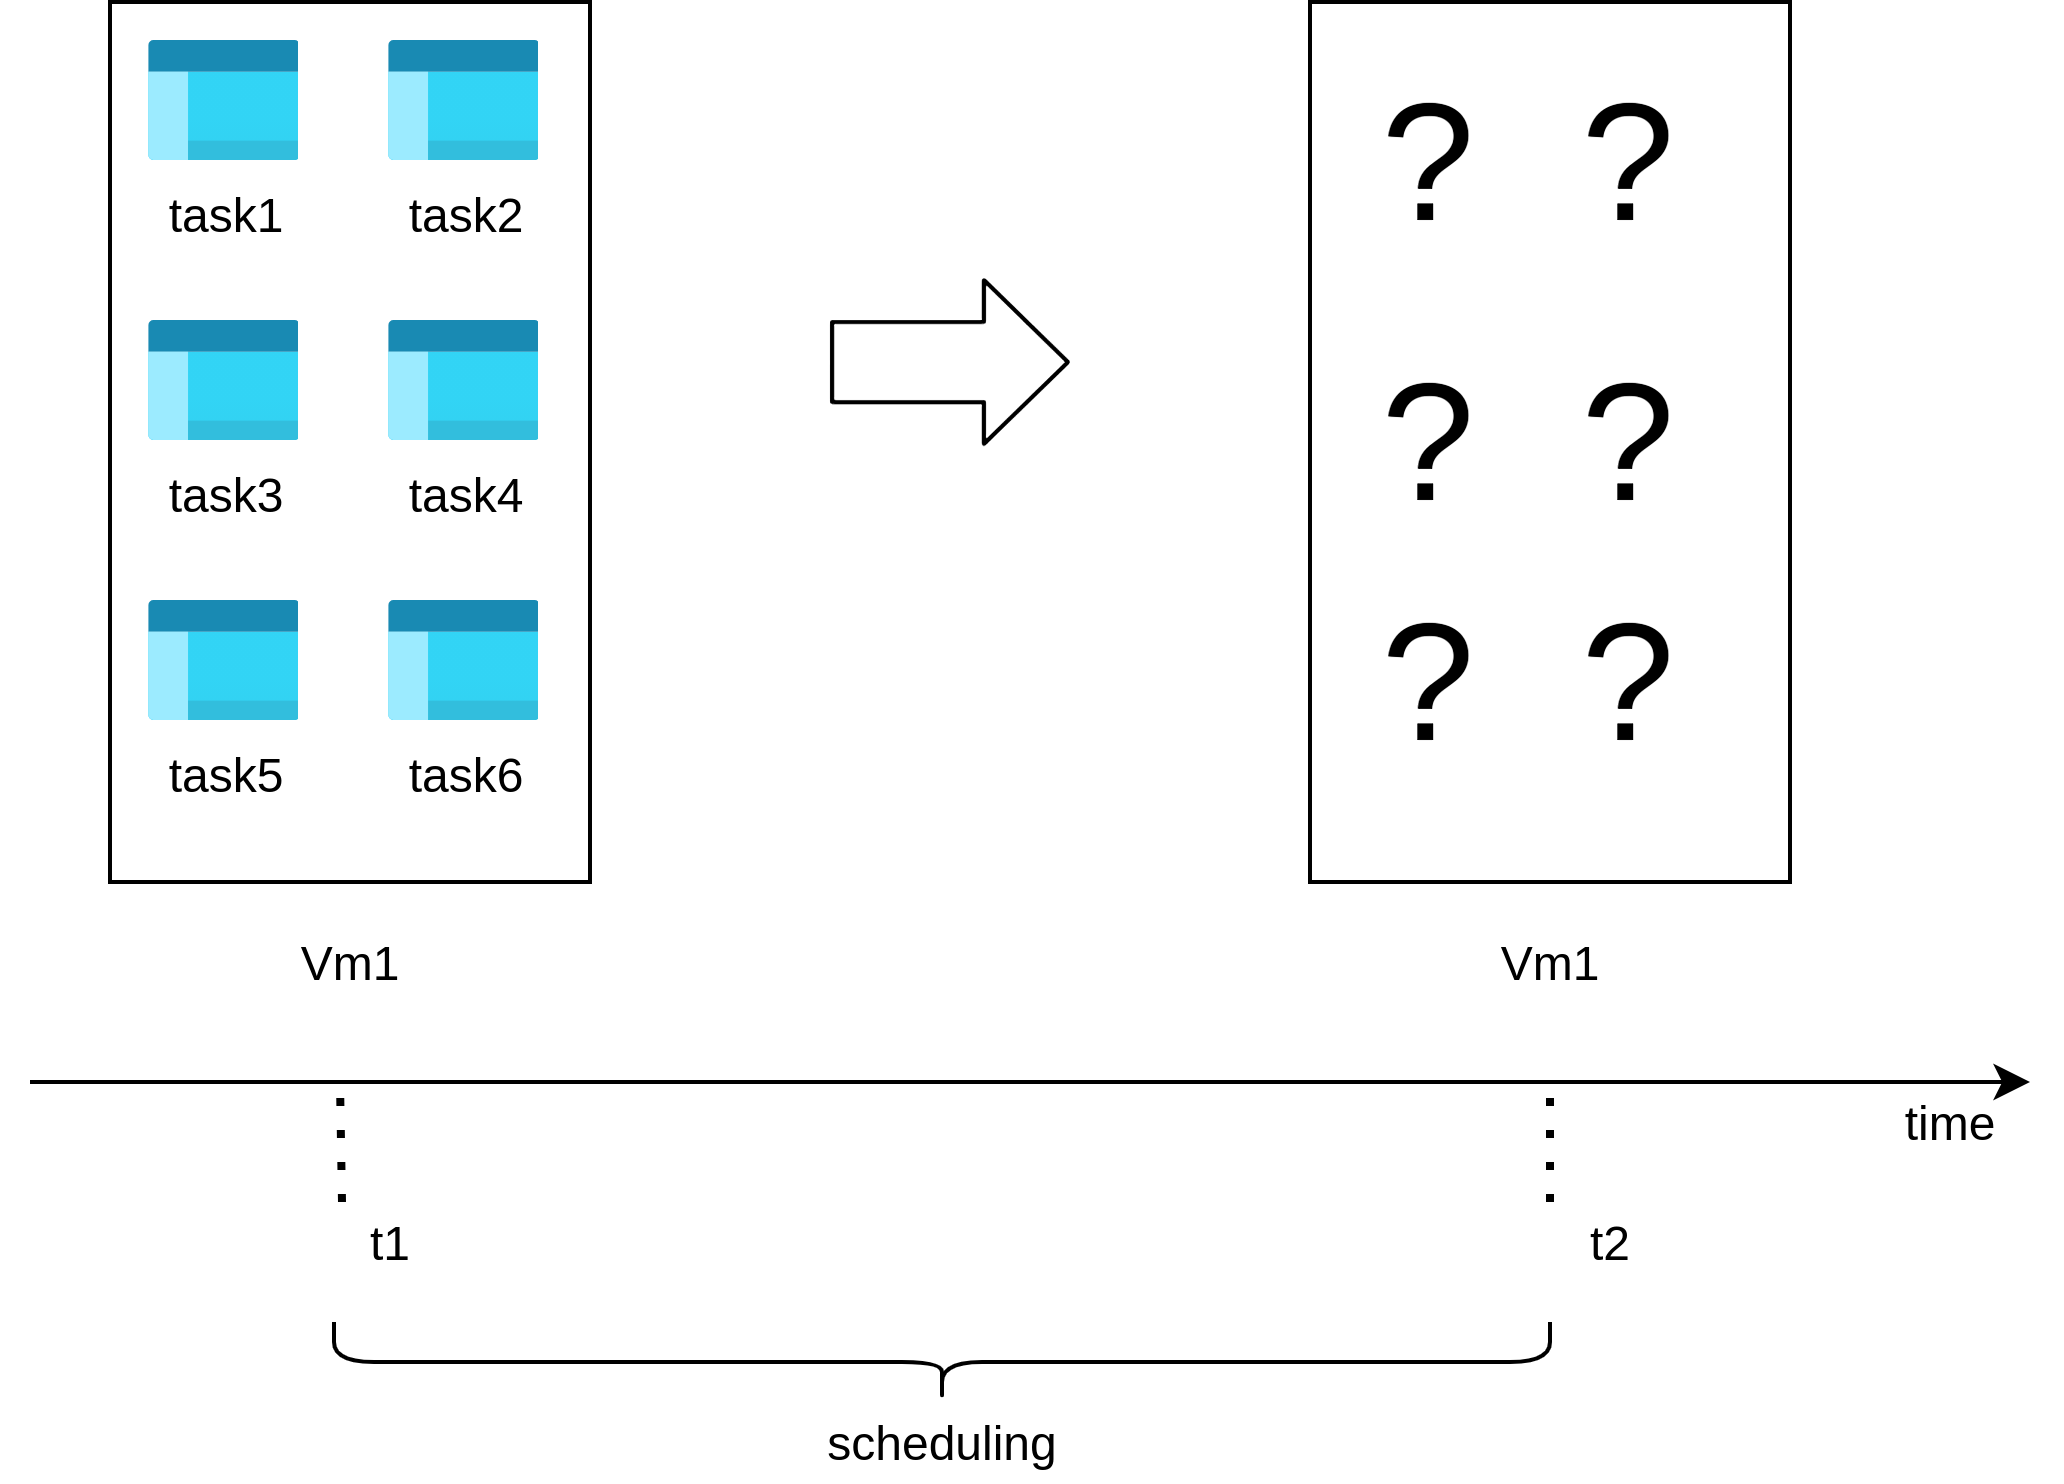
\includegraphics[scale=0.5]{images/predicting_status2.png}
%	\caption{Trạng thái tài nguyên tại thời điểm lập lịch và thực thi}
%\end{figure}
%\end{frame}

\begin{frame}
{Ước lượng trạng thái các tasks}
\begin{figure}
	\centering
	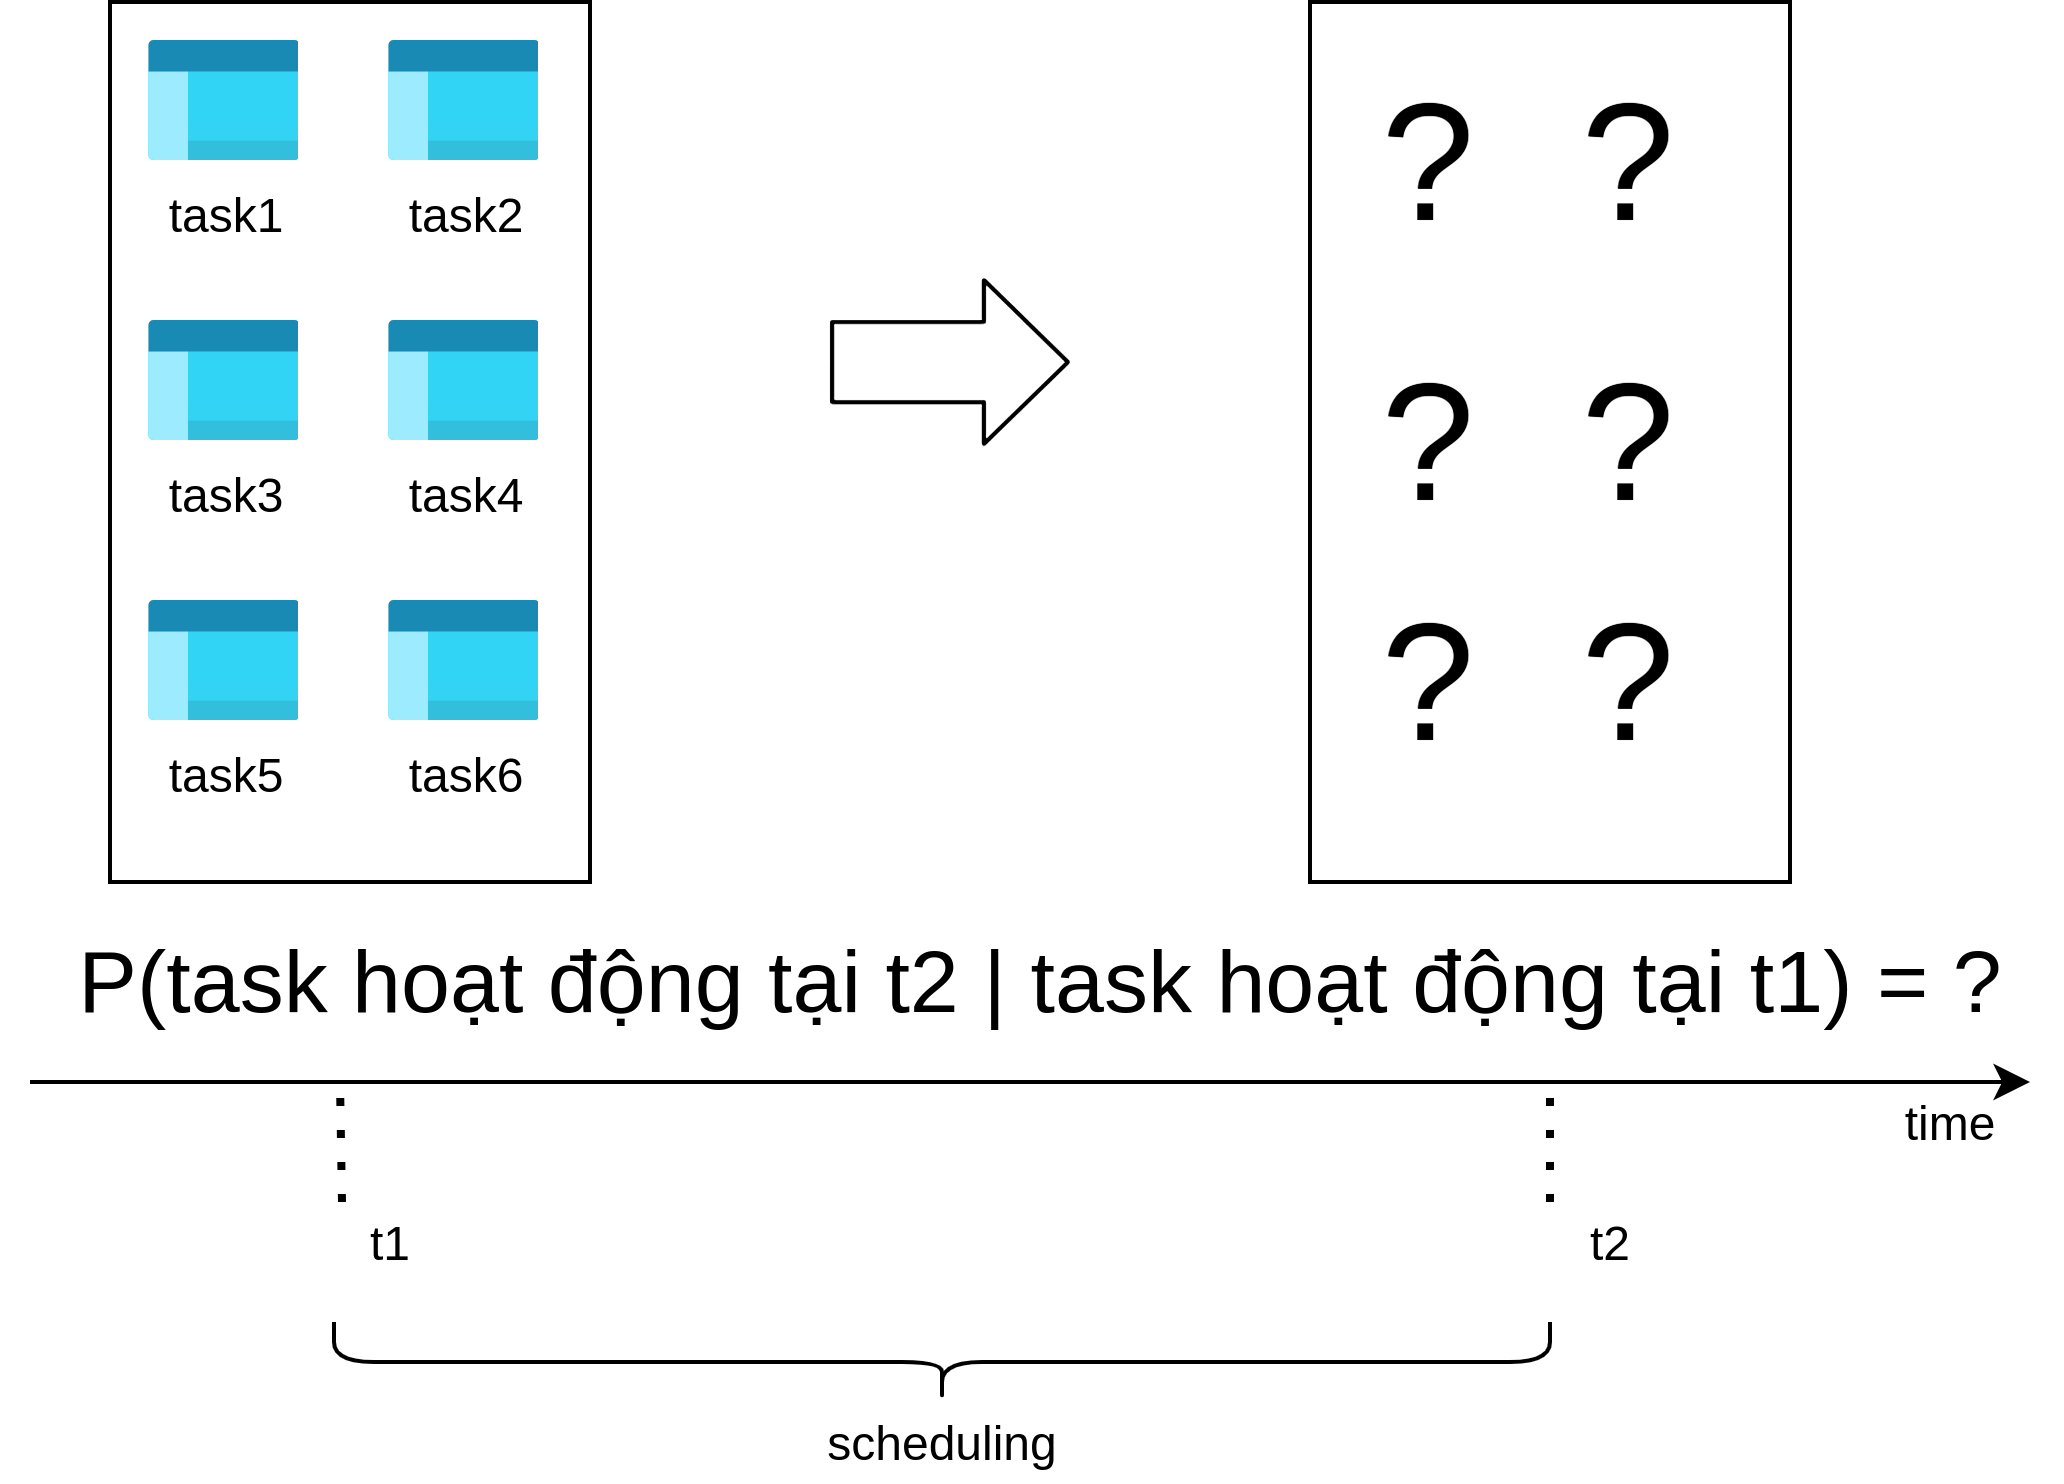
\includegraphics[scale=0.5]{images/predicting_status3.png}
\end{figure}
\begin{center}
	\large{Xác định xác suất tasks đang chạy còn hoạt động sau quá trình lập lịch để ước lượng trạng thái của máy ảo tại thời điểm thực thi}
\end{center}
\end{frame}

\begin{frame}
{Ước lượng tài nguyên khả dụng}
\pause
{Tập các tasks đang chạy trên máy tính ảo tại thời điểm lập lịch}
\[
	\mathcal{T} = \{task_{1}, task_{2}, ..., task_{K}\}
\]
Kỳ vọng tài nguyên sử dụng của một task: 
\begin{equation}
	E[task\_usage_{i}] = resources\_usage_{i} \times p_{i} + 0 * (1 - p_{i})
\end{equation}
\begin{itemize}
	\item $resources\_usage_{i}$ là tài nguyên $task_{i}$ sử dụng 
	\item $p_{i}$ là xác suất $task_{i}$ còn hoạt động tại thời điểm thực thi
\end{itemize}
Kì vọng tài nguyên khả dụng tại thời điểm thực thi: 
\begin{equation}
	available\_resources = resources\_capacity - \sum_{i = 1}^{K}{resources\_usage_{i} \times p_{i}}
\end{equation}
\end{frame}

\begin{frame}
{Ví dụ minh họa mạng Bayesian}
	\begin{figure}
		\centering
		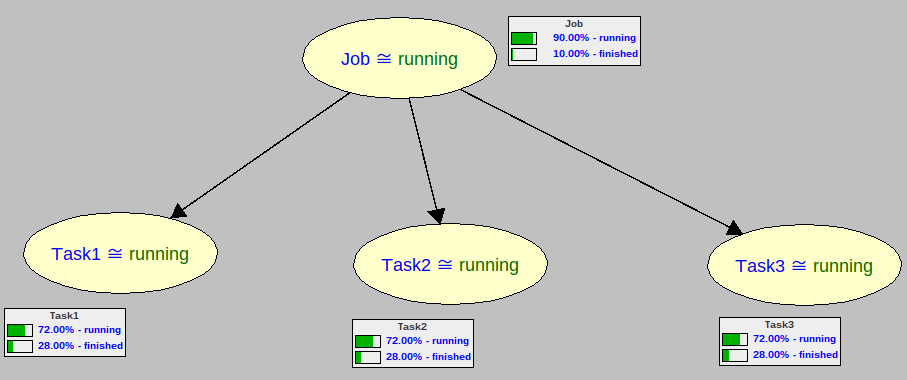
\includegraphics[scale=0.4]{images/bayesian_network_ex1.png}
		\caption{Ví dụ về mạng Bayesian cho 3 tasks}
	\end{figure}
\end{frame}

\begin{frame}
{Ví dụ minh họa mạng Bayesian}
	\begin{figure}
		\centering
		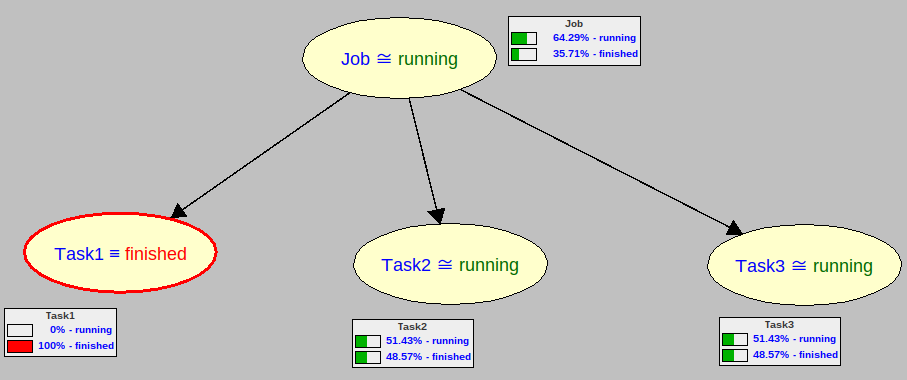
\includegraphics[scale=0.4]{images/bayesian_network_ex2.png}
		\caption{Ví dụ về mạng Bayesian cho 3 tasks}
	\end{figure}
\end{frame}

\begin{frame}
{Ví dụ minh họa mạng Bayesian}
	\begin{figure}
		\centering
		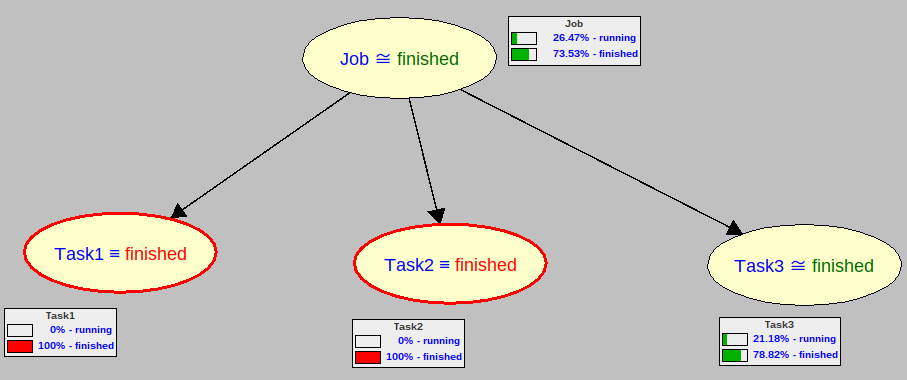
\includegraphics[scale=0.4]{images/bayesian_network_ex3.png}
		\caption{Ví dụ về mạng Bayesian cho 3 tasks}
	\end{figure}
\end{frame}

\begin{frame}
{Cân bằng khối lượng công việc giữa các máy ảo}
% Đề xuất thuật toán cân bằng khối lượng công việc giữa các máy ảo 
\pause
\begin{block}
{Độ mất cân bằng}
Khối lượng công việc của M máy ảo: 
\begin{center}
	$\mathcal{L} = \{l_{1}, l_{2}, ..., l_{M}\}$
\end{center}
Để thể hiện độ mất cân bằng khối lượng công việc giữa các máy ảo, ta sử dụng phương sai của $\mathcal{L}$
\begin{center}
	$\mathcal{V}(\mathcal{L}) = \frac{1}{M} \times \sum_{i = 1}^{M}(l_{i} - \overline{l})^{2}$
\end{center}
\end{block}
\begin{block}
{Mục tiêu của thuật toán lập lịch}
Tối thiểu hóa độ mất cân bằng của hệ thống \textbf{trong thời gian hoạt động}.
\end{block}
\end{frame}

\begin{frame}
{Lựa chọn máy tính ảo cho tasks}
	\begin{figure}
		\vspace{1cm}
		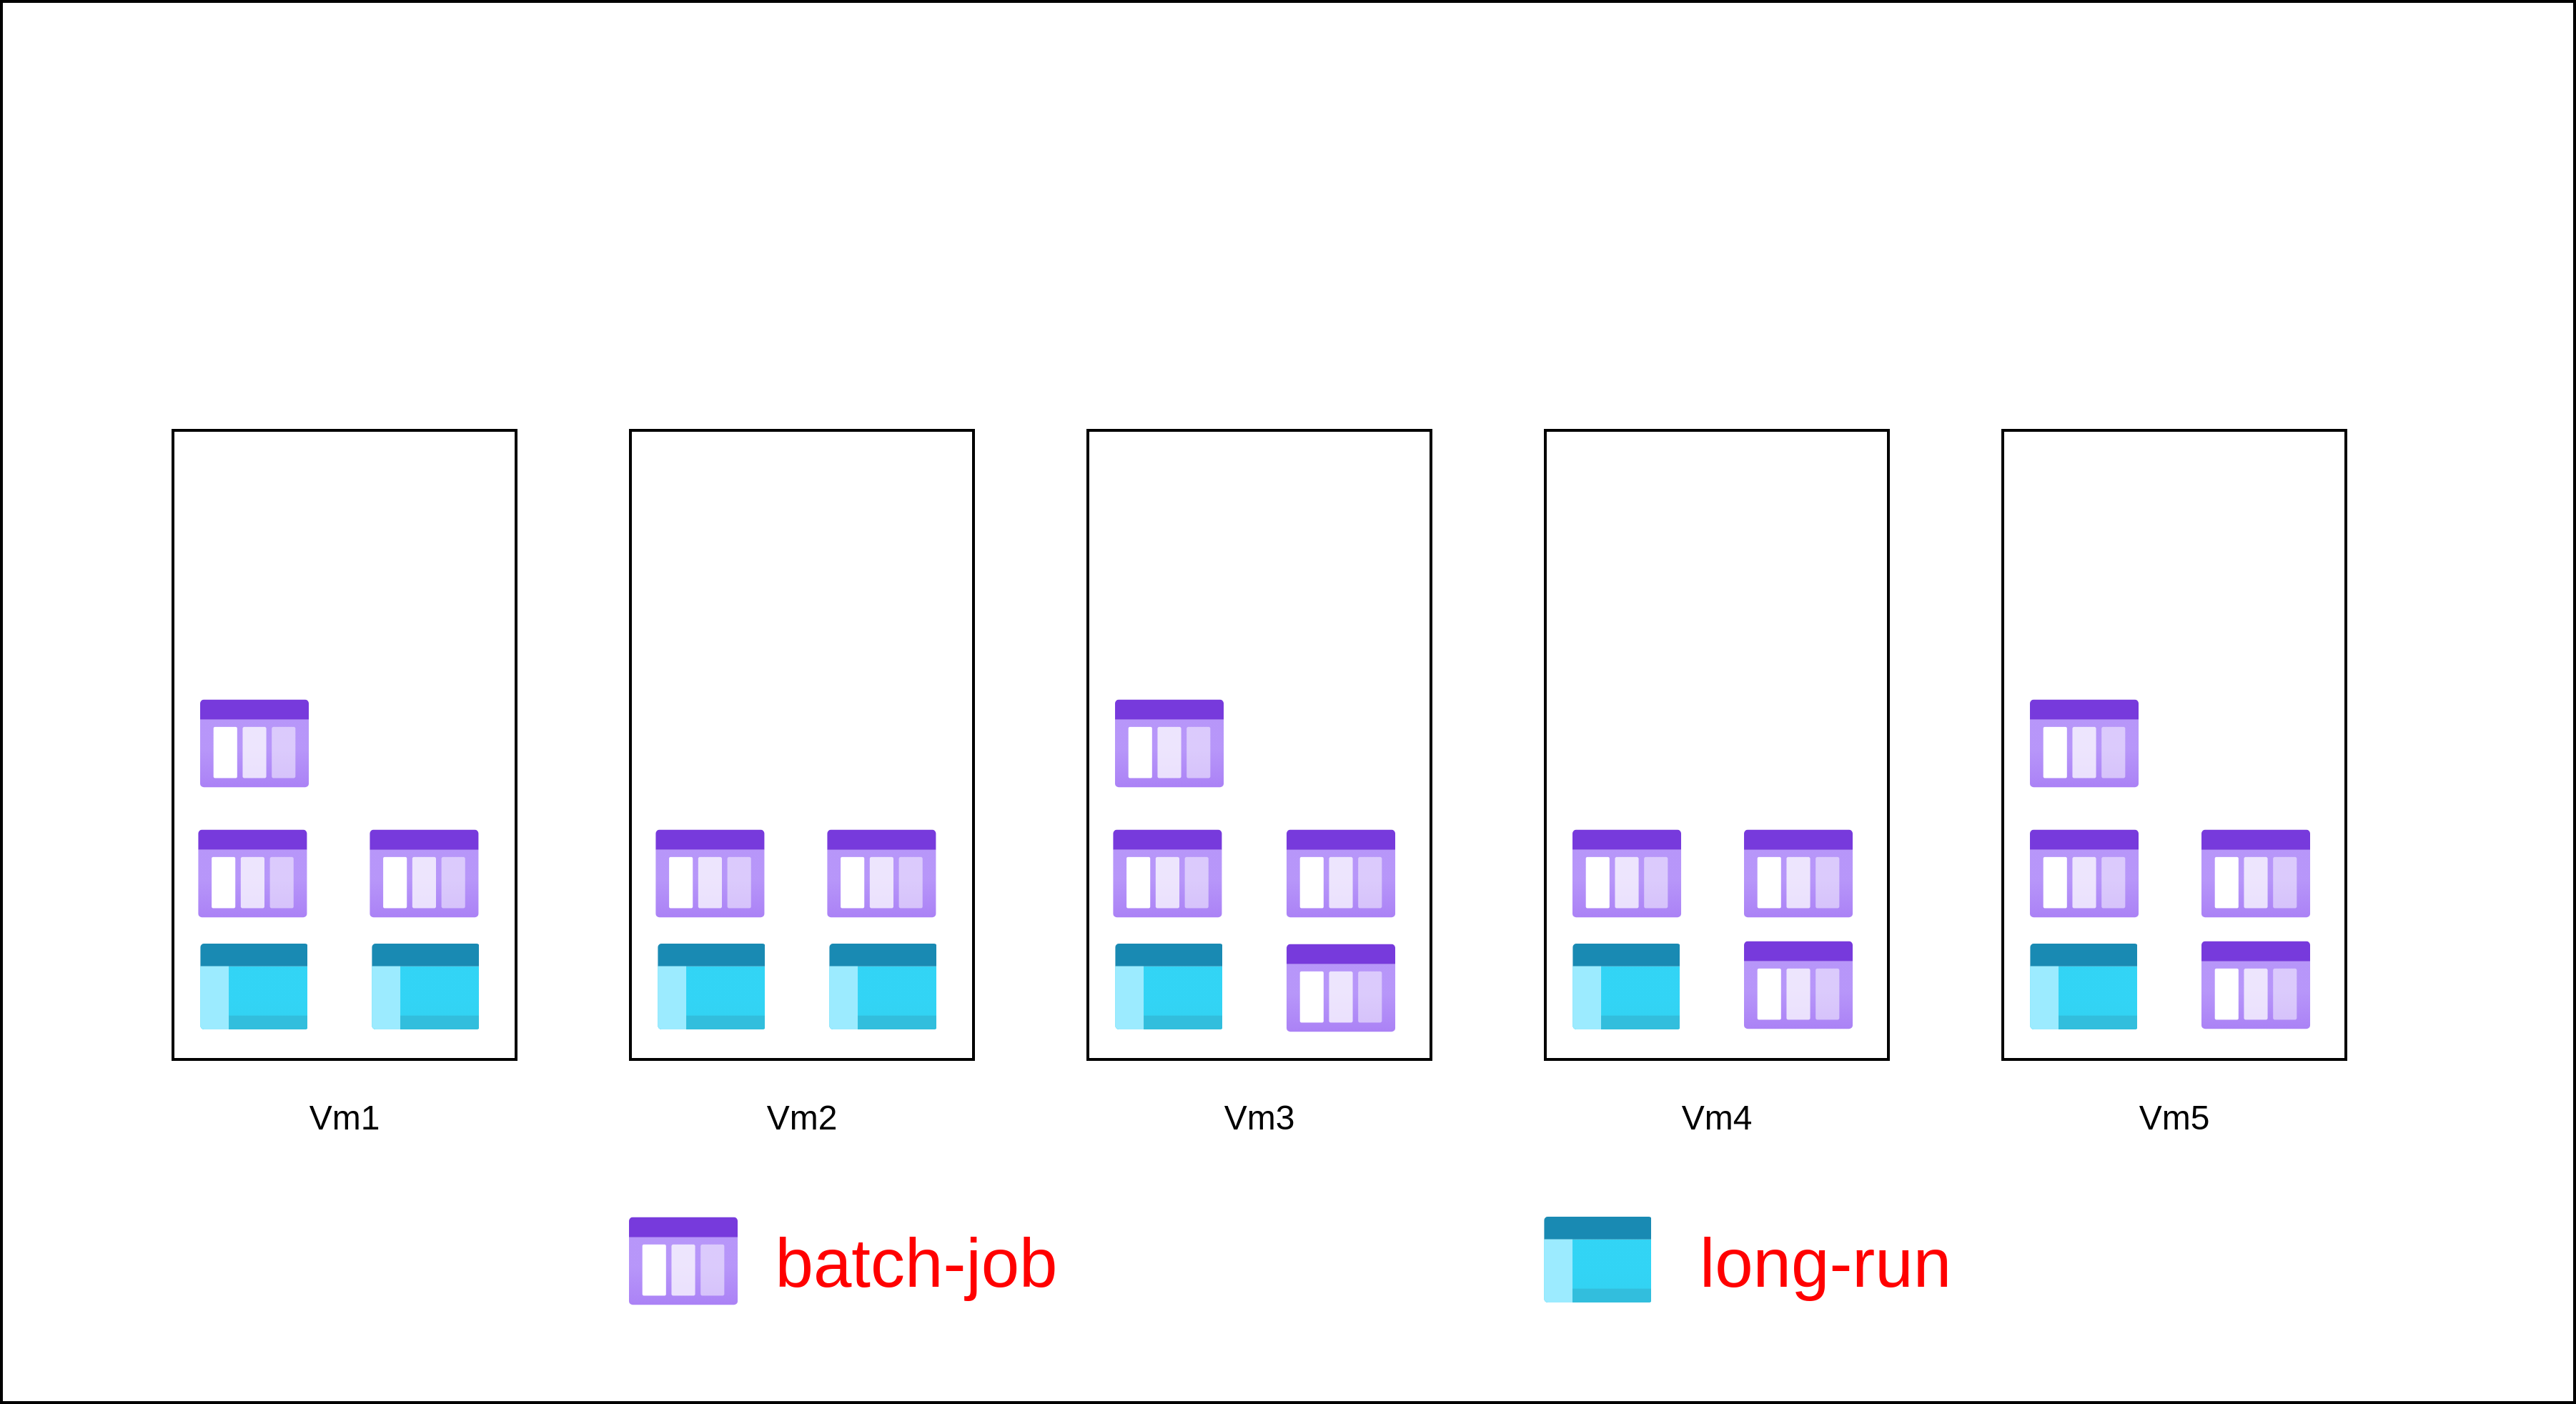
\includegraphics[scale=0.4]{images/balancing_tasks1.png}
%		\caption{Lập lịch cho tasks}
	\end{figure}
\end{frame}

\begin{frame}
{Lựa chọn máy tính ảo cho tasks}

	\begin{minipage}[t]{0.4\linewidth}
		\vspace{0.5cm}
		Tìm máy ảo cho long-run task: 
		\begin{itemize}
			\item Bước 1: Chọn K máy ảo có lượng tài nguyên dành cho long-run tasks nhỏ nhất 
			\item Bước 2: Trong K máy ảo tìm được, chọn máy có lượng tài nguyên khả dụng cao nhất cho task 
			\item Bước 3: Cập nhật thông tin task được ghép cặp với máy ảo
		\end{itemize}
	\end{minipage}
	\hfill
	\begin{minipage}[t]{0.59\linewidth}
	\begin{figure}
		\vspace{1cm}
		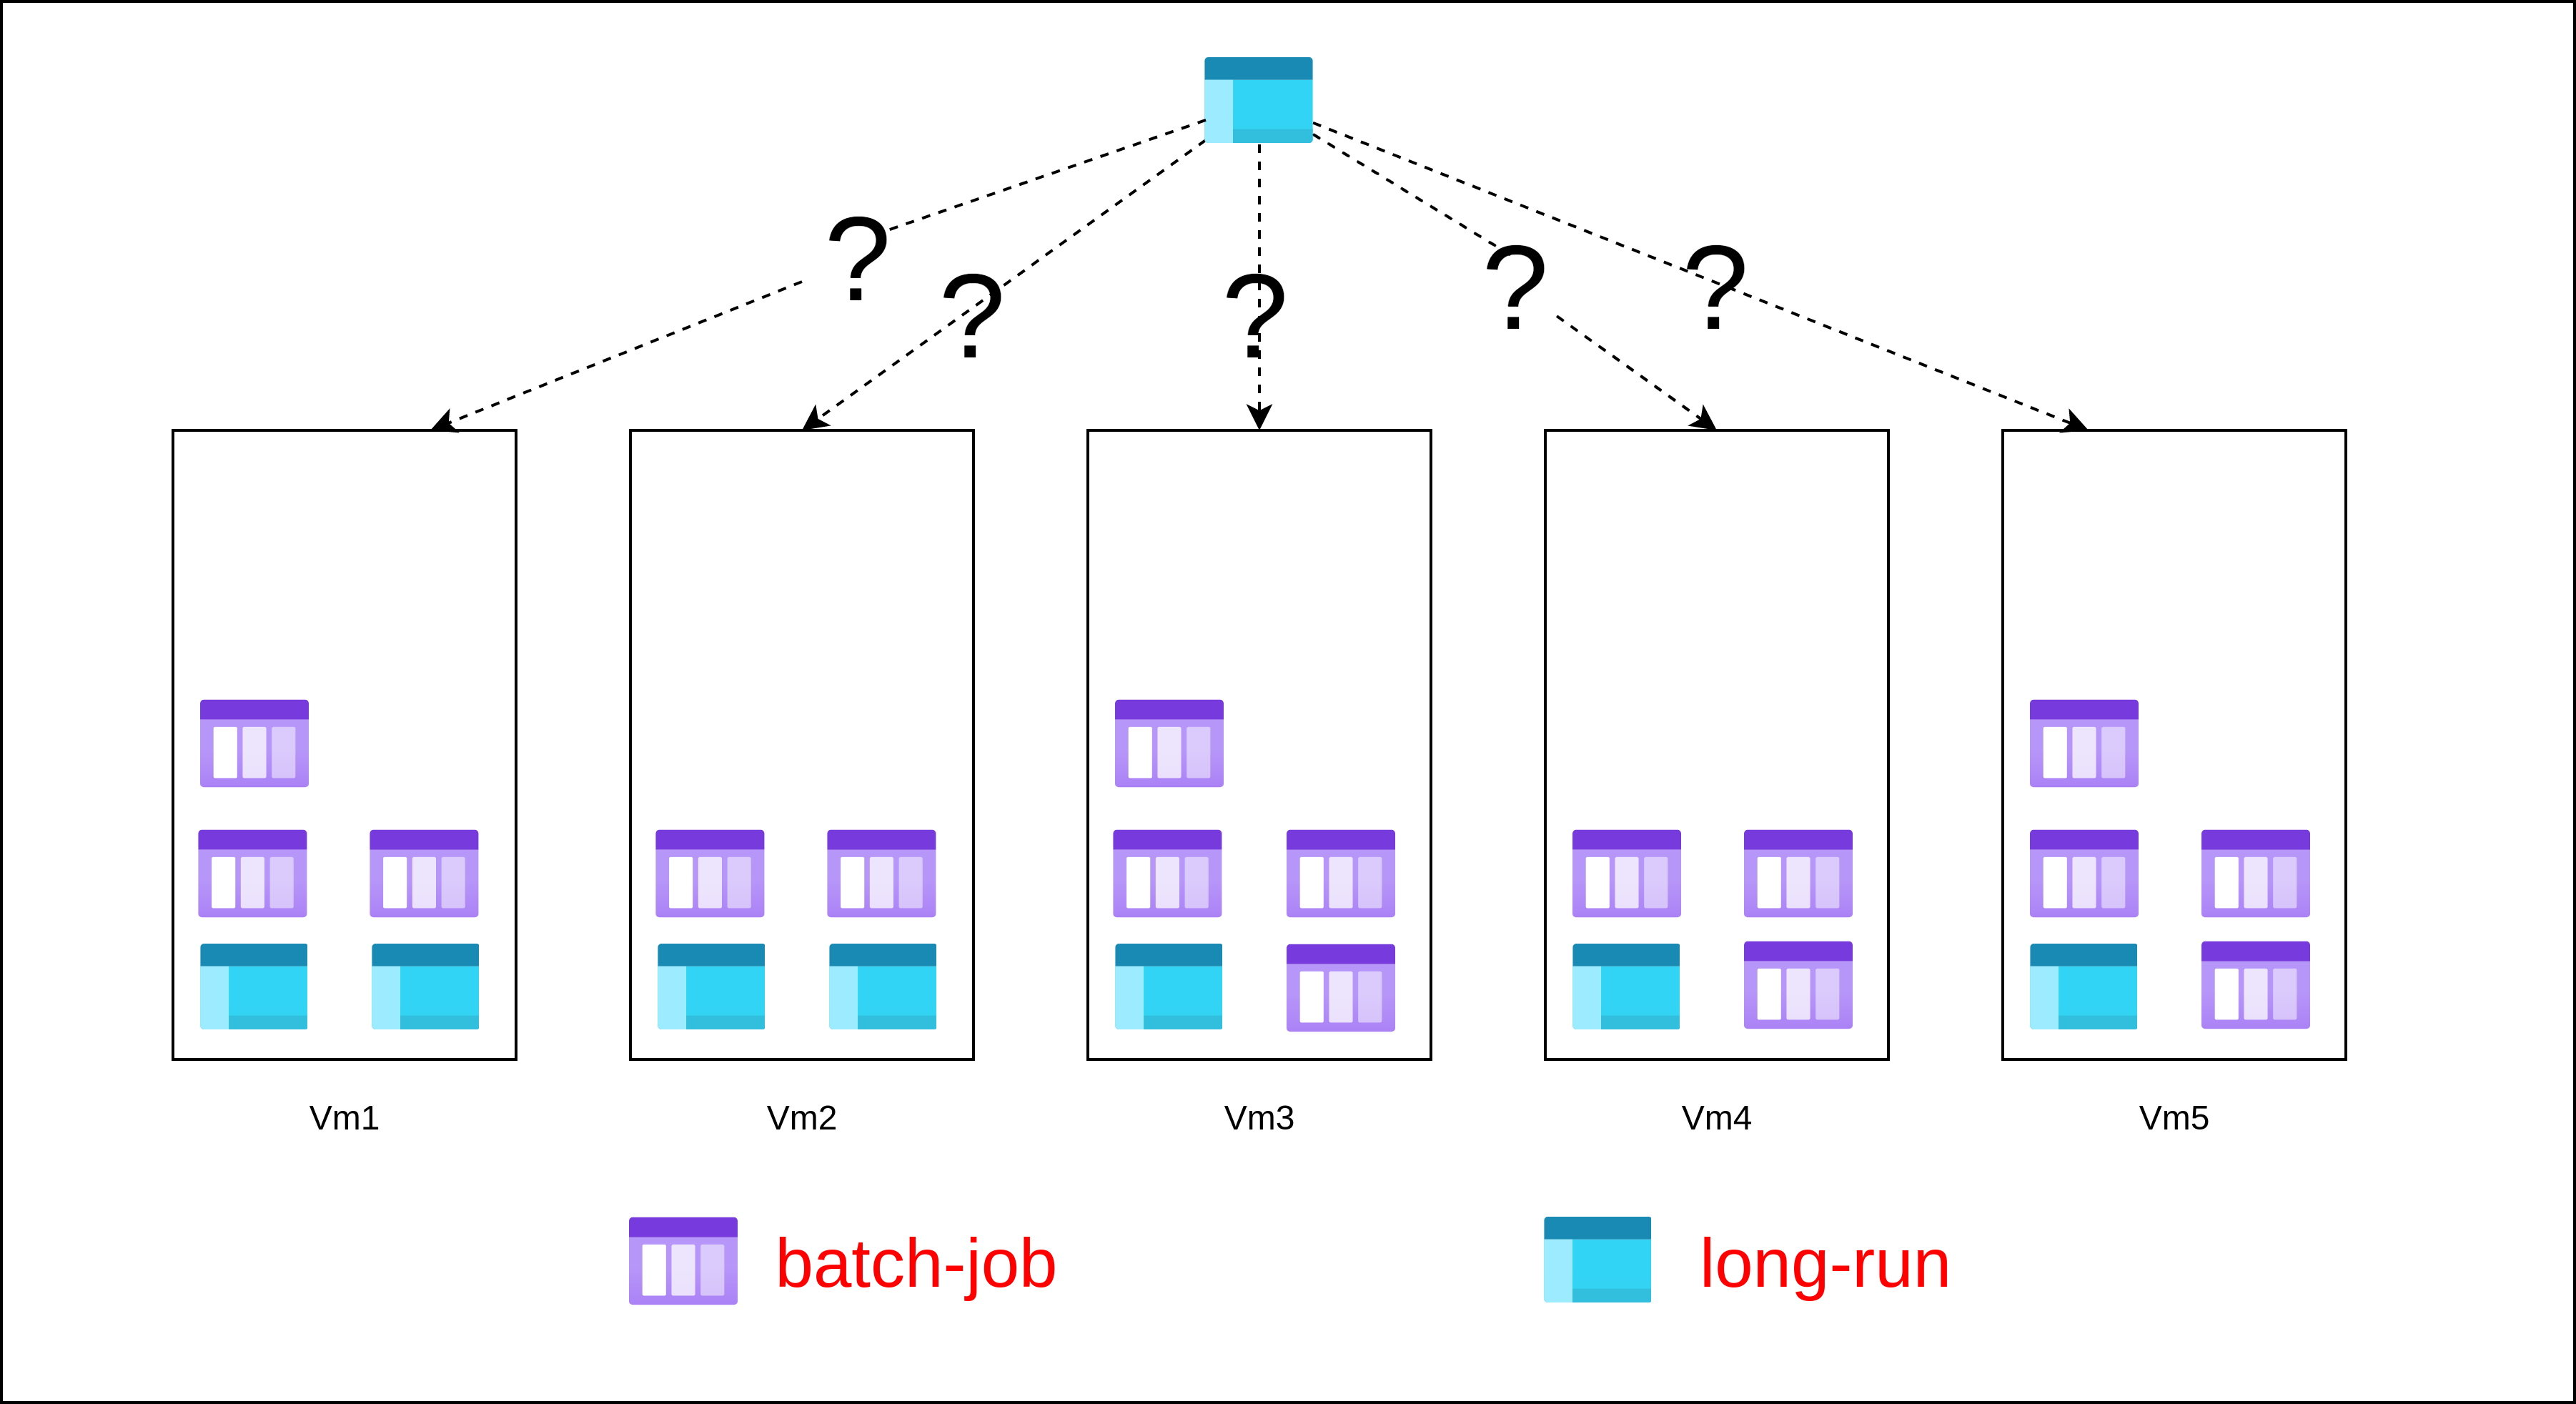
\includegraphics[scale=0.35]{images/balancing_tasks2.png}
%		\caption{Lập lịch cho tasks}
	\end{figure}
	\vspace{1cm}
	\end{minipage}
\end{frame}

\begin{frame}
{Lựa chọn máy tính ảo cho tasks}

	\begin{minipage}[t]{0.4\linewidth}
		\vspace{0.5cm}
		Tìm máy ảo cho long-run task: 
		\begin{itemize}
			\item {\color{red}{Bước 1}}: Chọn K máy ảo có lượng tài nguyên dành cho long-run tasks nhỏ nhất 
			\item Bước 2: Trong K máy ảo tìm được, chọn máy có lượng tài nguyên khả dụng cao nhất cho task 
			\item Bước 3: Cập nhật thông tin task được ghép cặp với máy ảo
		\end{itemize}
	\end{minipage}
	\hfill
	\begin{minipage}[t]{0.59\linewidth}
	\begin{figure}
		\vspace{1cm}
		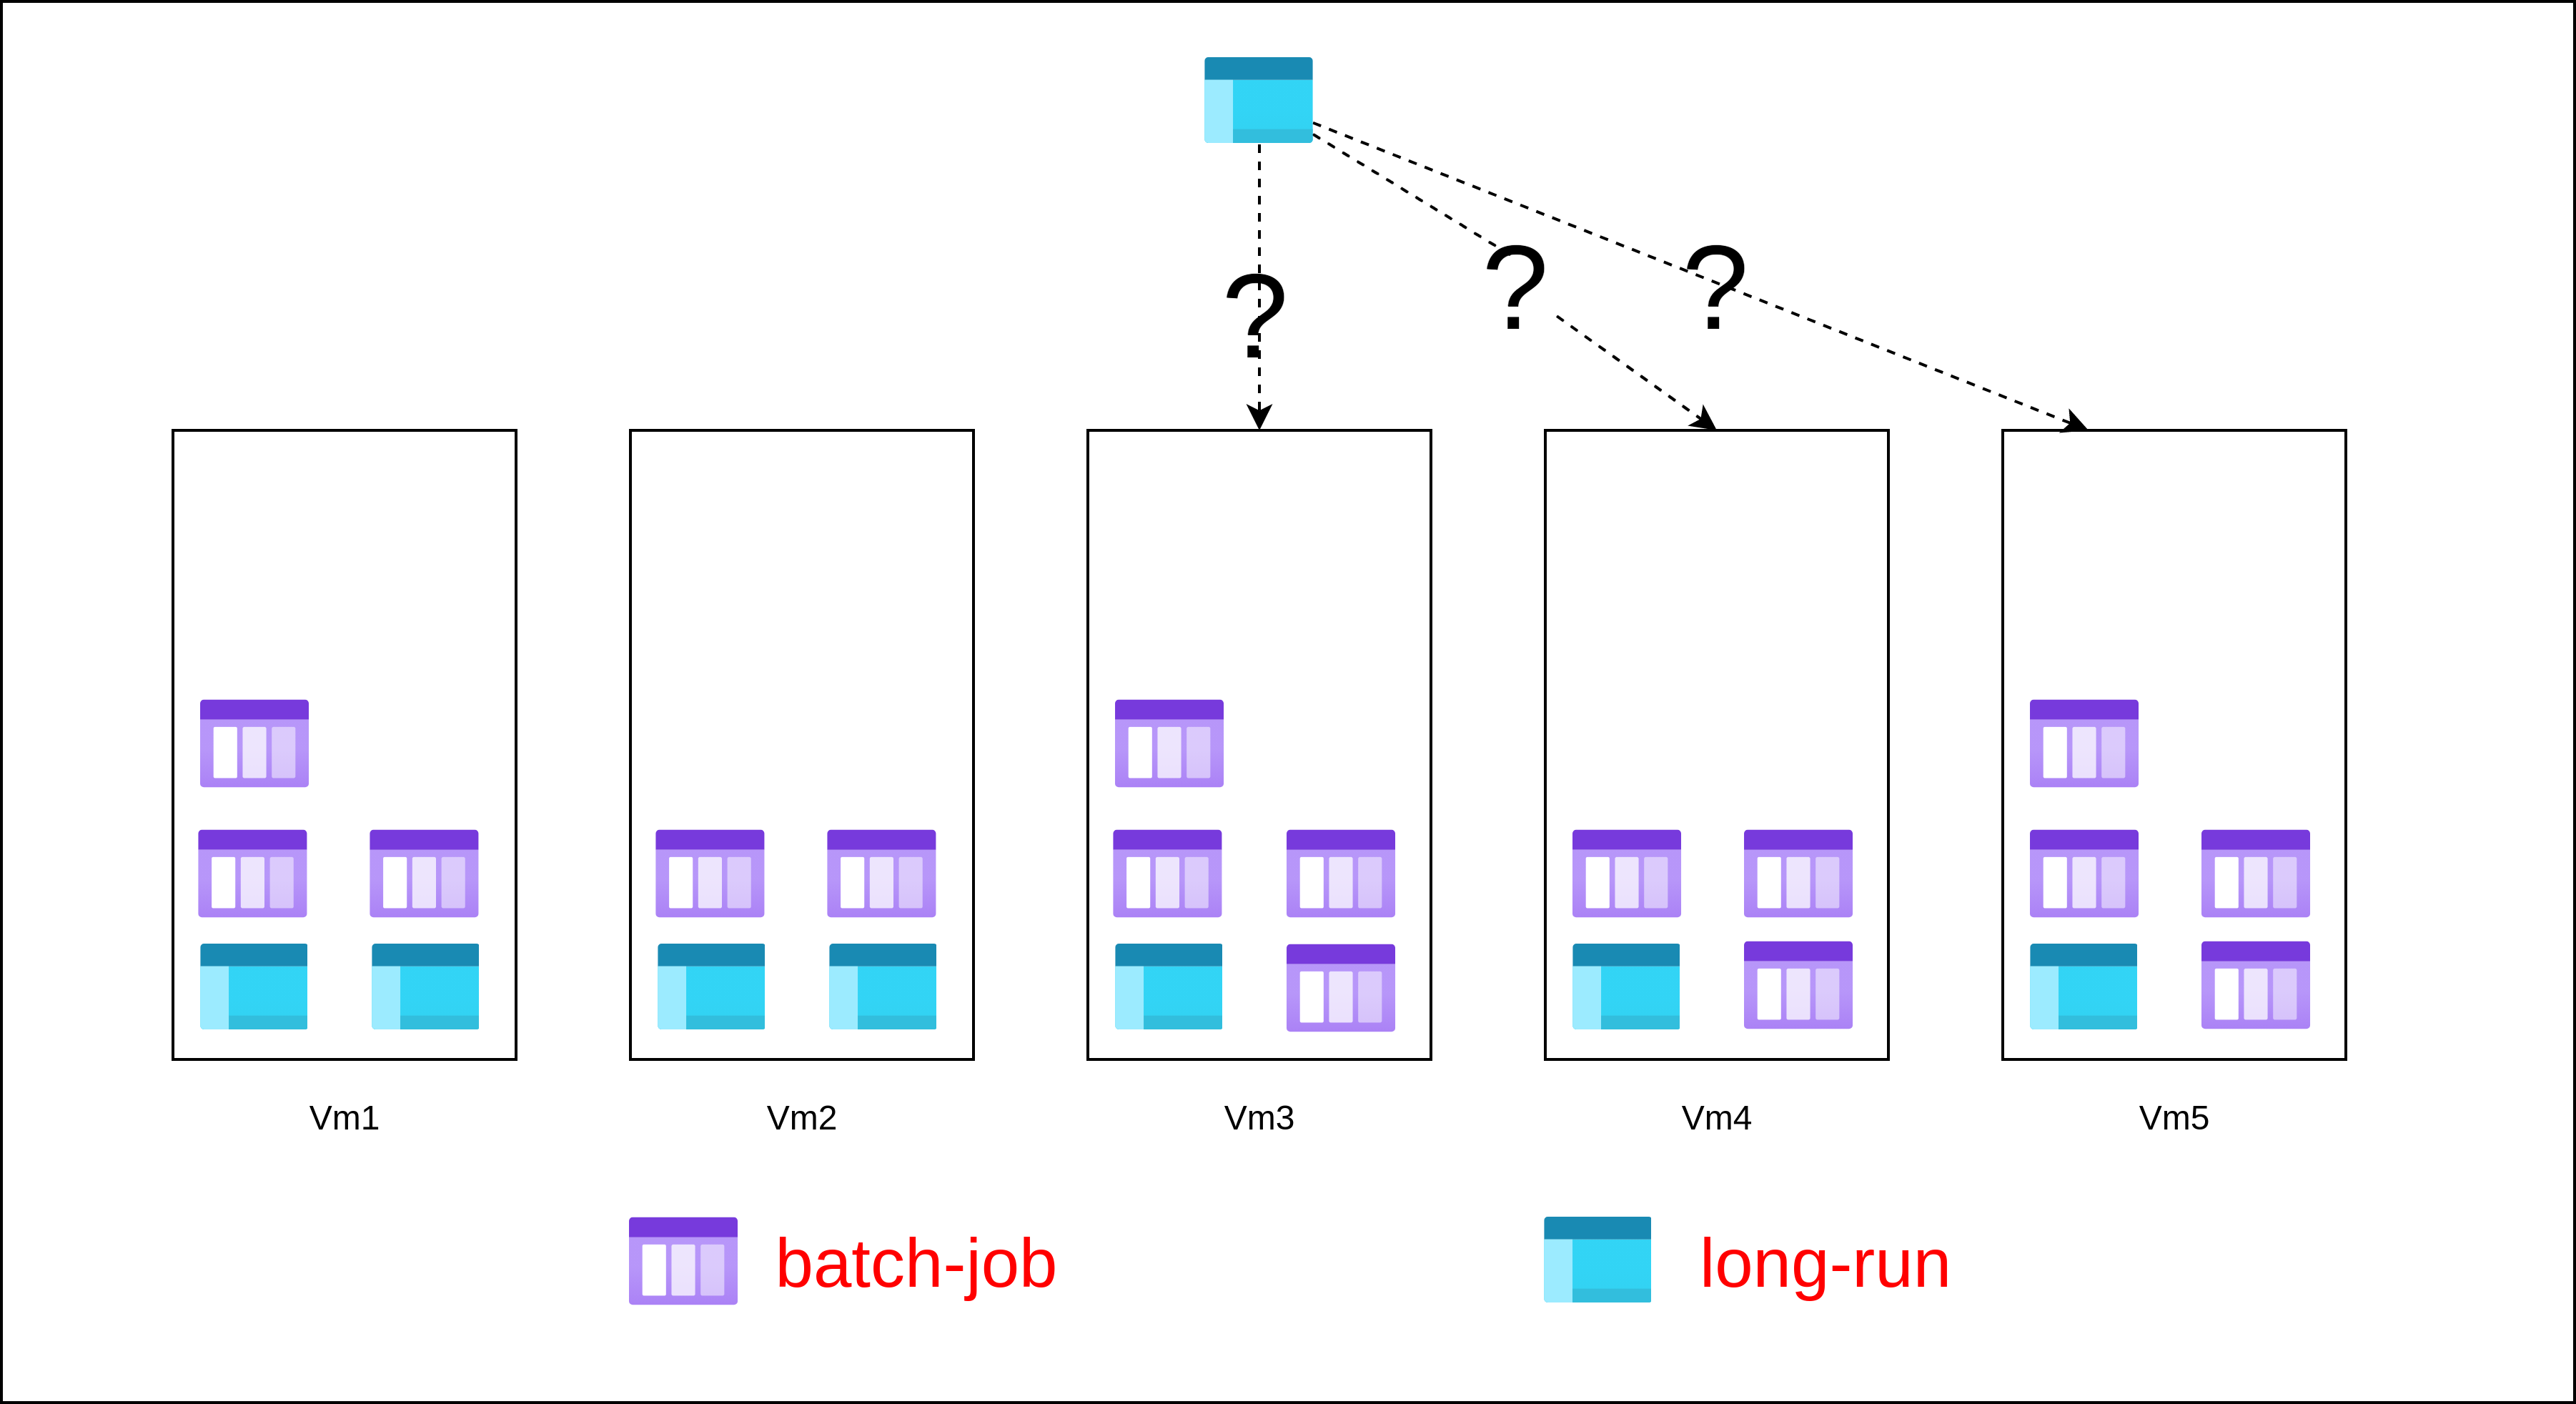
\includegraphics[scale=0.35]{images/balancing_tasks3.png}
%		\caption{Lập lịch cho tasks}
	\end{figure}
	\vspace{1cm}
	\end{minipage}
\end{frame}

\begin{frame}
{Lựa chọn máy tính ảo cho tasks}

	\begin{minipage}[t]{0.4\linewidth}
		\vspace{0.5cm}
		Tìm máy ảo cho long-run task: 
		\begin{itemize}
			\item Bước 1: Chọn K máy ảo có lượng tài nguyên dành cho long-run tasks nhỏ nhất 
			\item {\color{red}{Bước 2}}: Trong K máy ảo tìm được, chọn máy có lượng tài nguyên khả dụng cao nhất cho task 
			\item Bước 3: Cập nhật thông tin task được ghép cặp với máy ảo
		\end{itemize}
	\end{minipage}
	\hfill
	\begin{minipage}[t]{0.59\linewidth}
	\begin{figure}
		\vspace{1cm}
		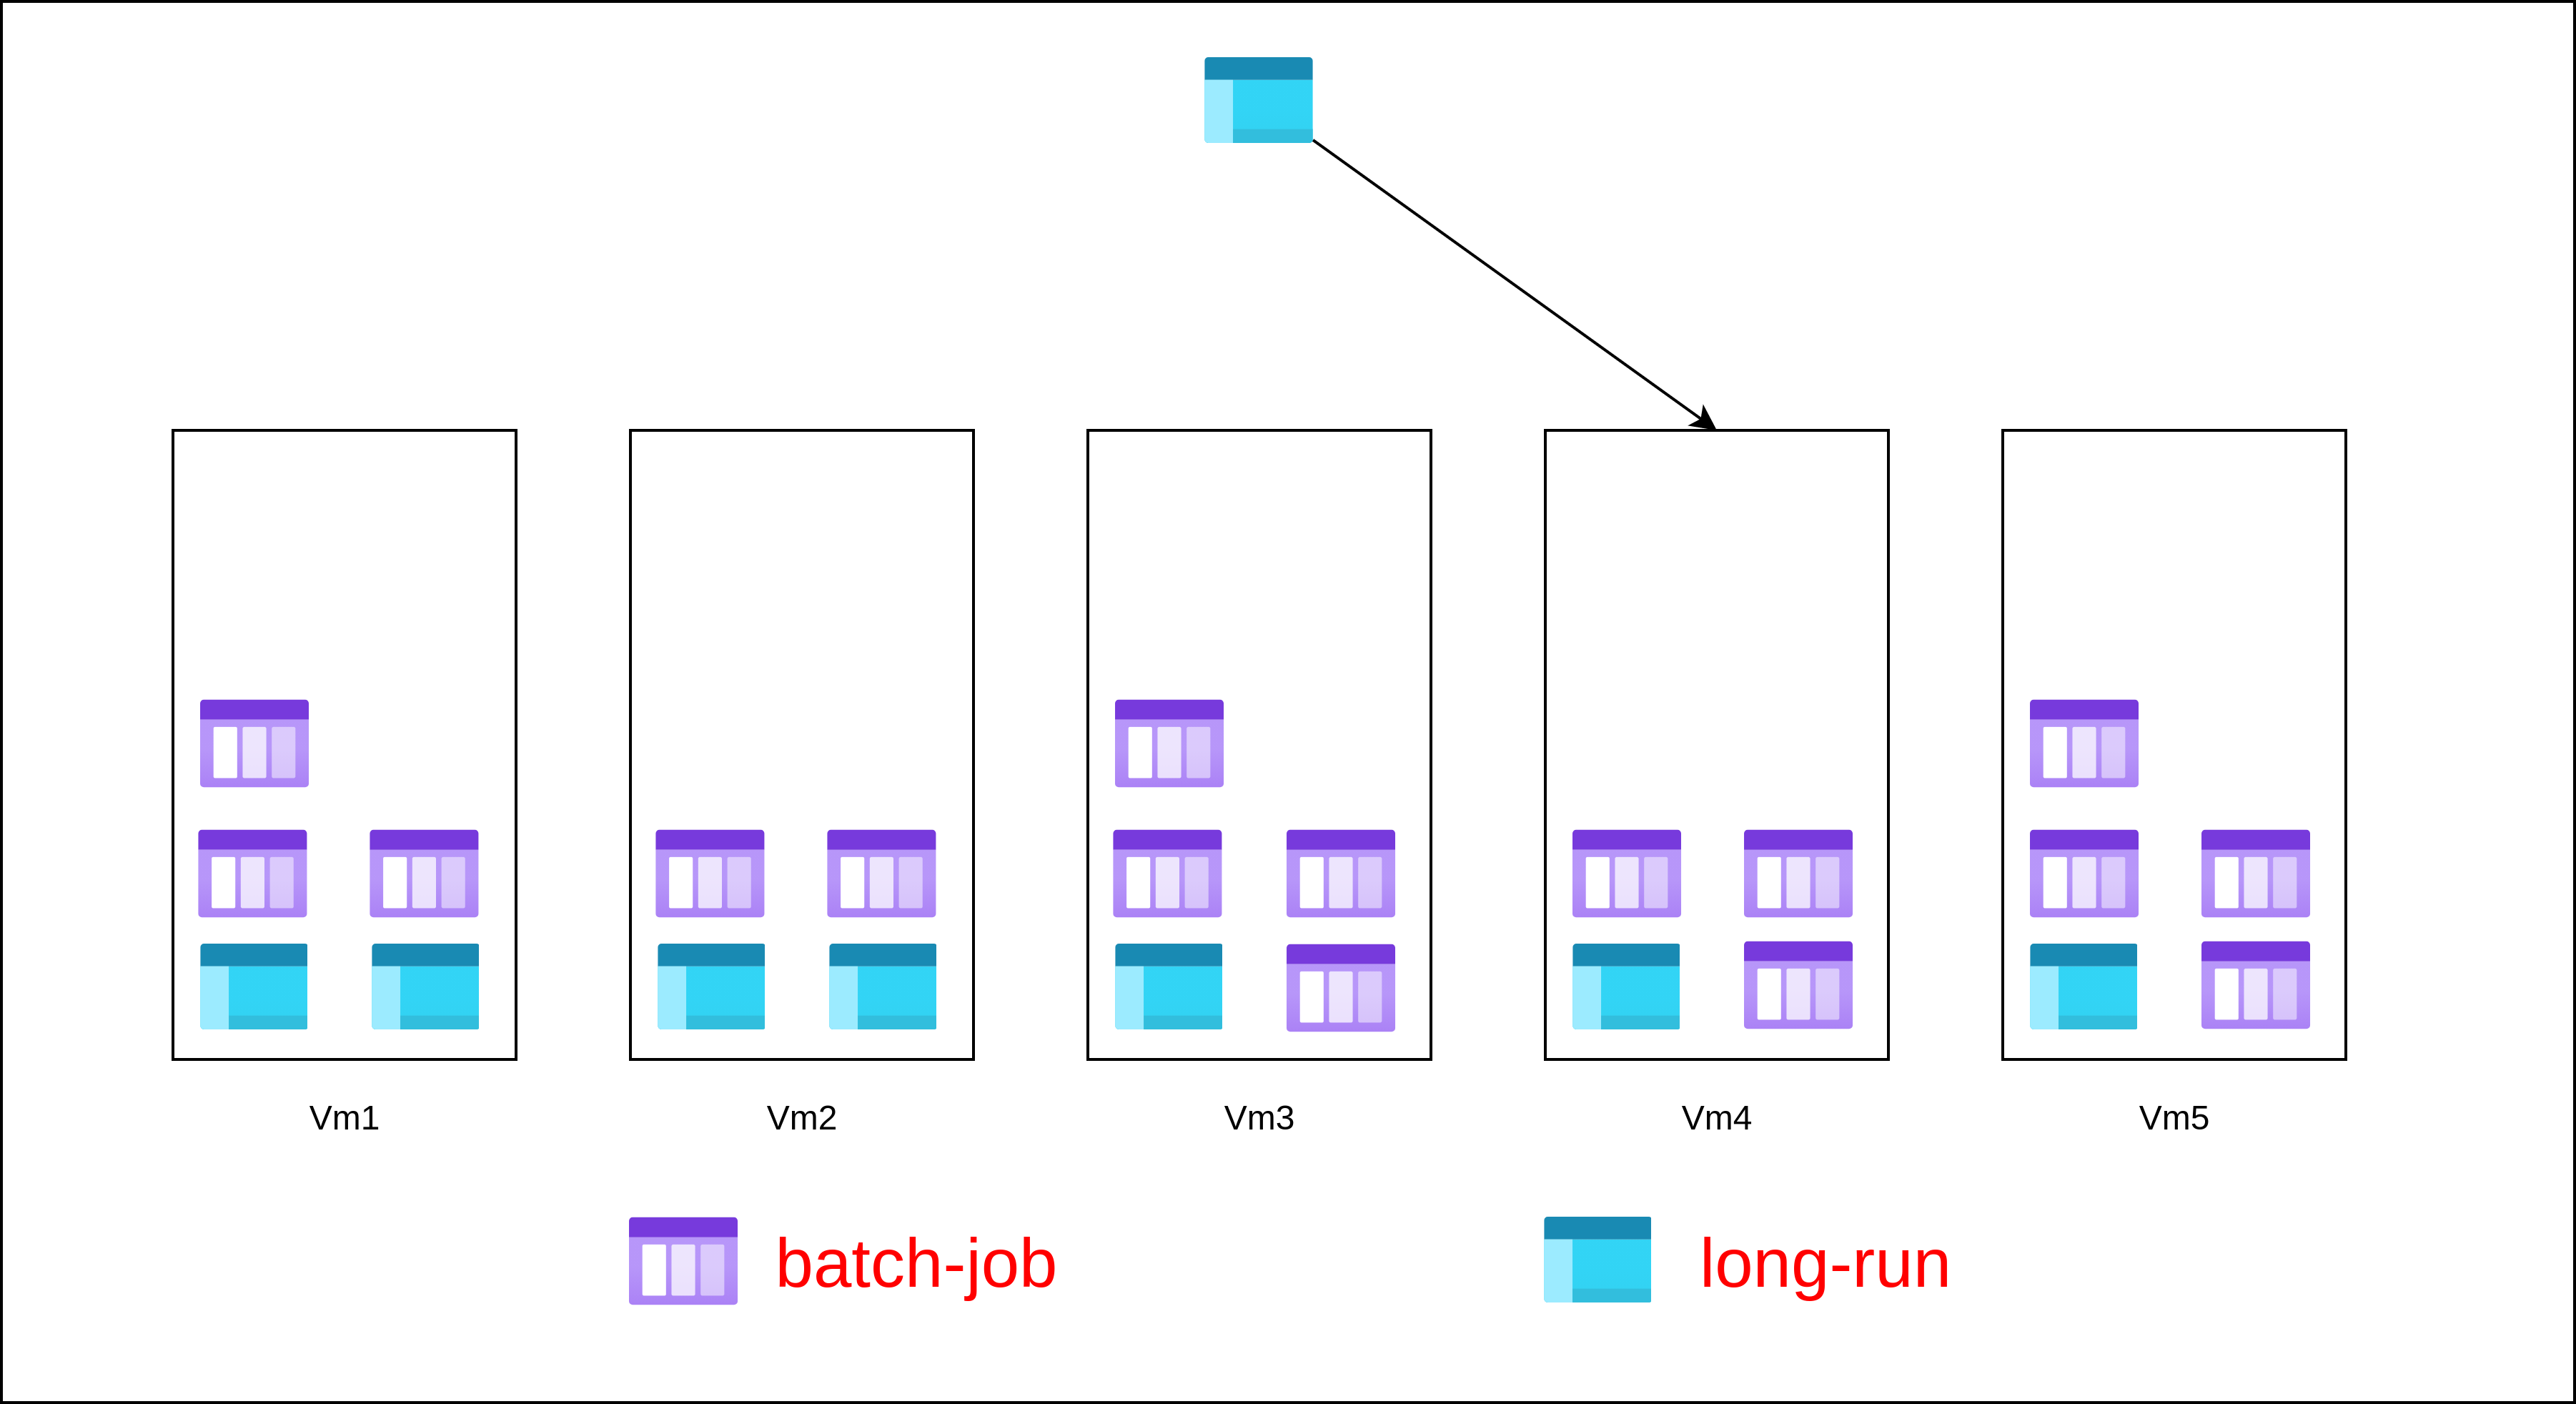
\includegraphics[scale=0.35]{images/balancing_tasks4.png}
%		\caption{Lập lịch cho tasks}
	\end{figure}
	\vspace{1cm}
	\end{minipage}
\end{frame}

\begin{frame}
{Lựa chọn máy tính ảo cho tasks}

	\begin{minipage}[t]{0.4\linewidth}
		\vspace{0.5cm}
		Tìm máy ảo cho long-run task: 
		\begin{itemize}
			\item Bước 1: Chọn K máy ảo có lượng tài nguyên dành cho long-run tasks nhỏ nhất 
			\item Bước 2: Trong K máy ảo tìm được, chọn máy có lượng tài nguyên khả dụng cao nhất cho task 
			\item {\color{red}{Bước 3}}: Cập nhật thông tin task được ghép cặp với máy ảo
		\end{itemize}
	\end{minipage}
	\hfill
	\begin{minipage}[t]{0.59\linewidth}
	\begin{figure}
		\vspace{1cm}
		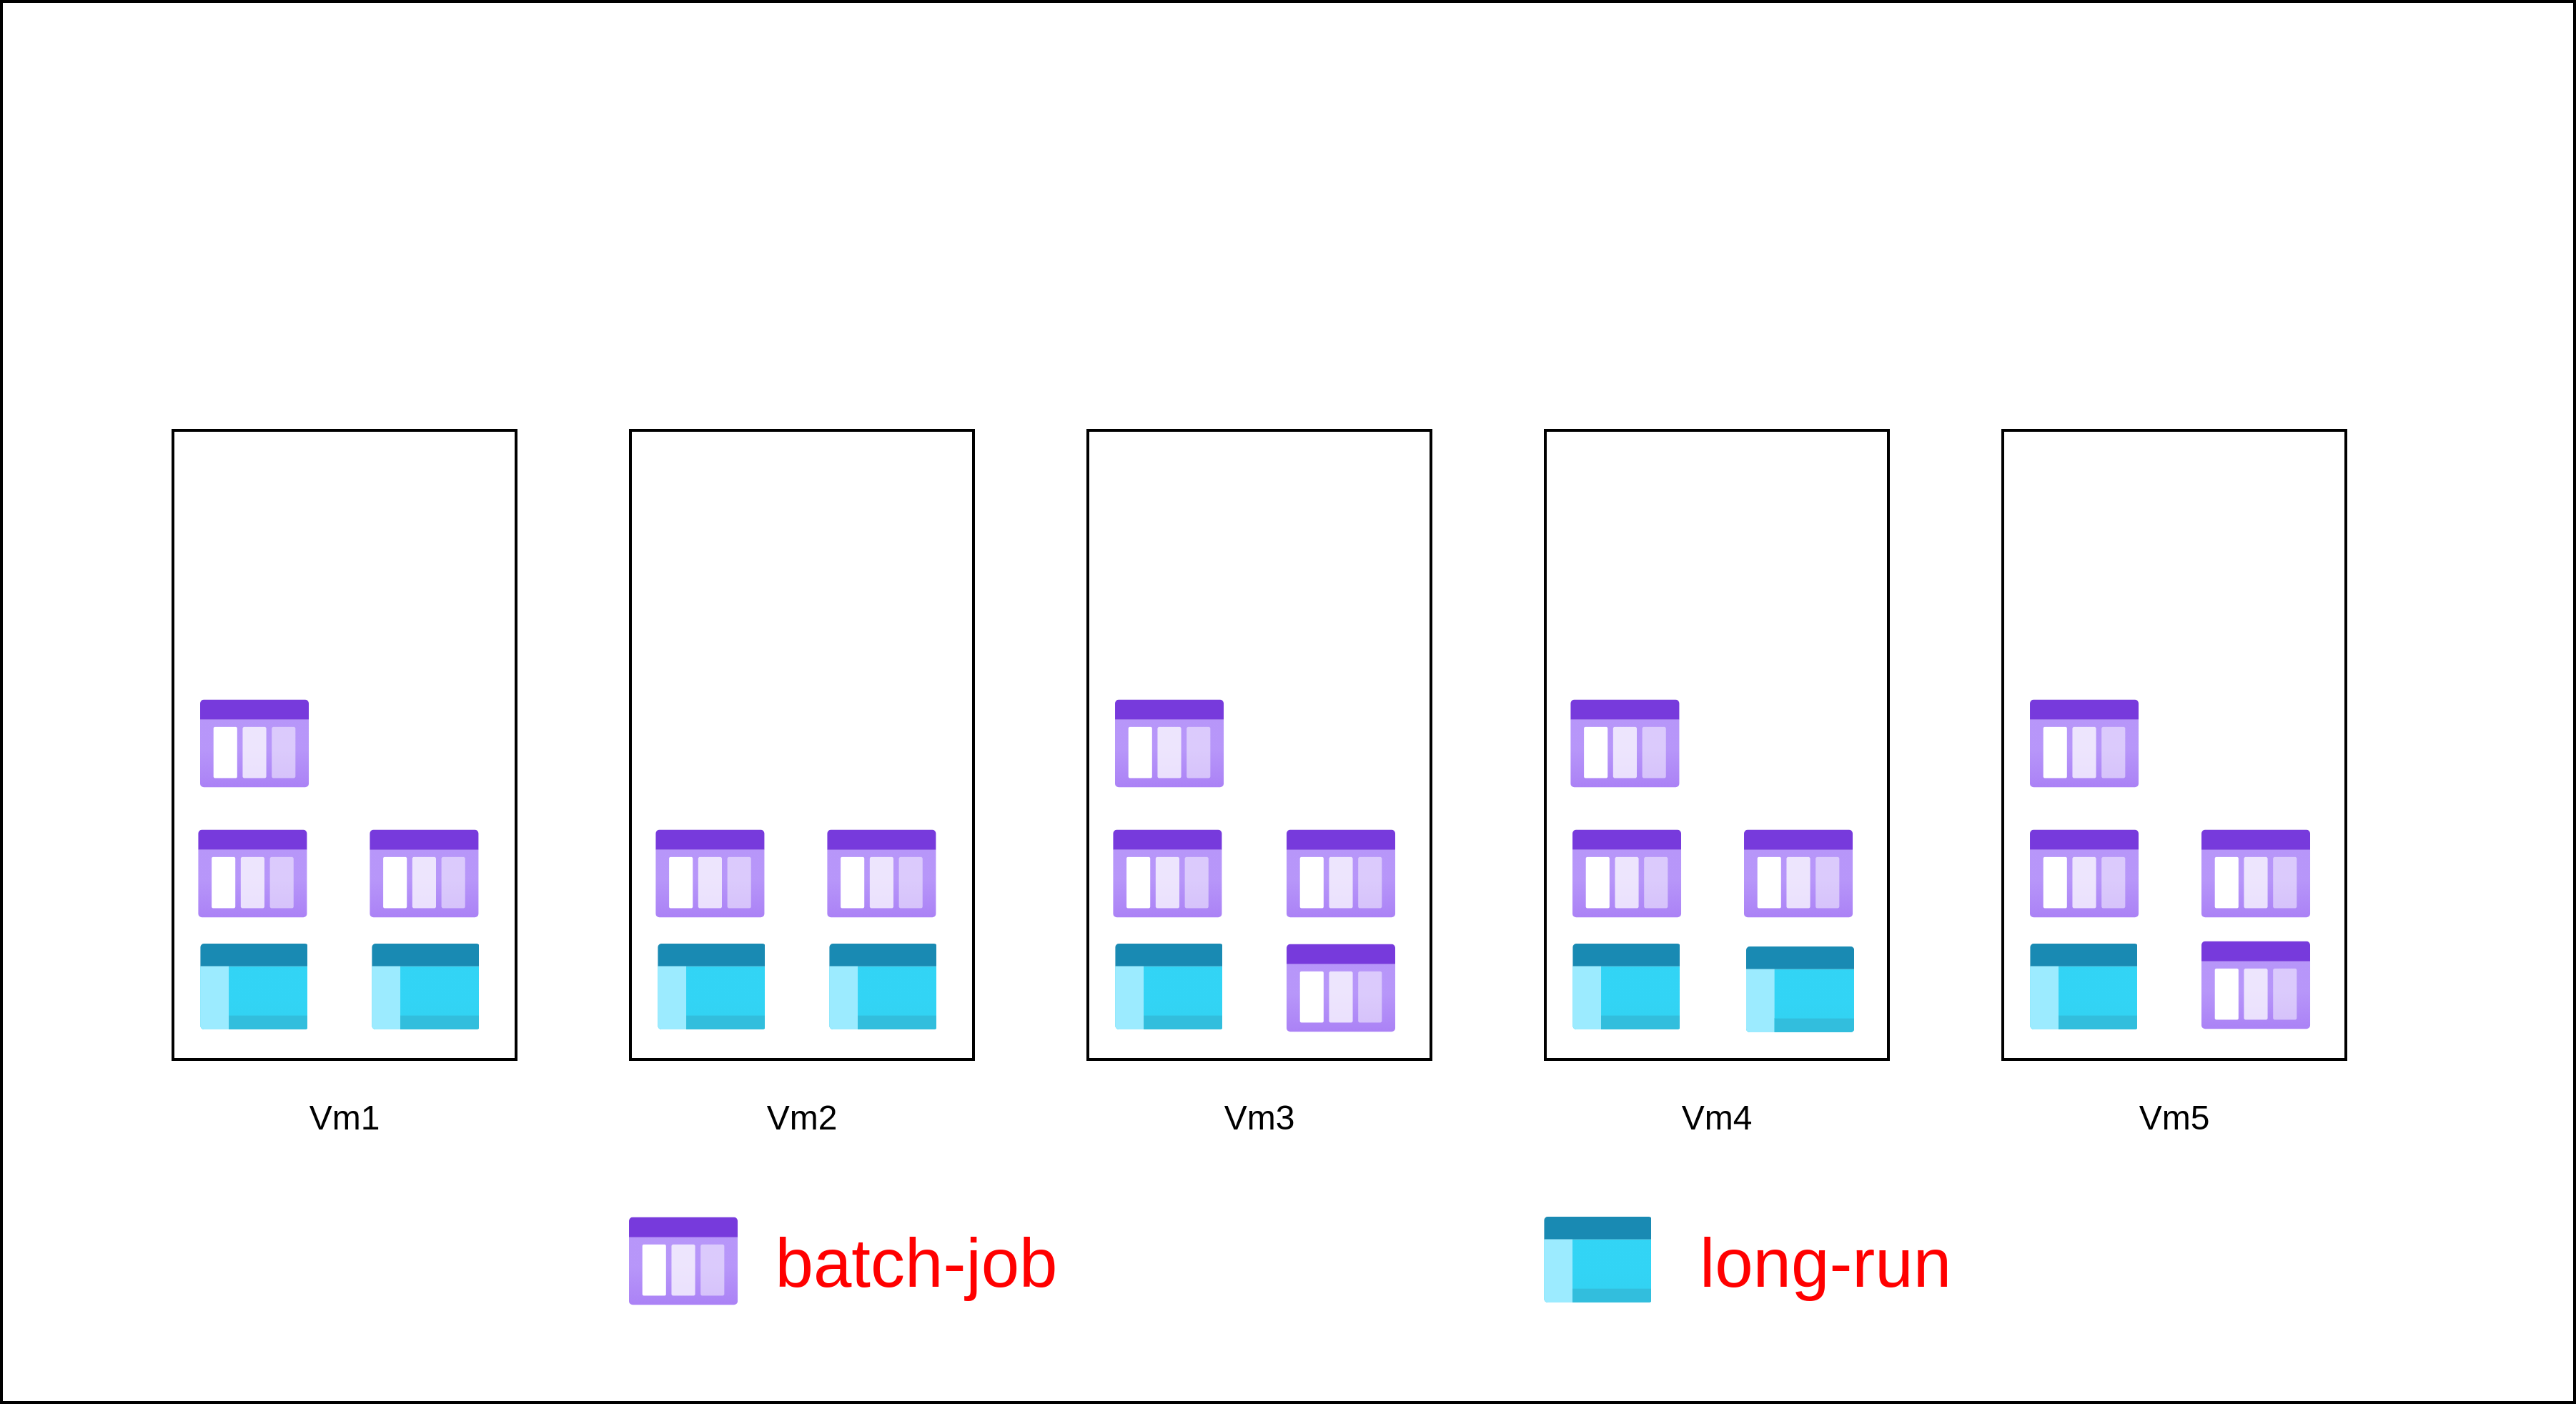
\includegraphics[scale=0.35]{images/balancing_tasks5.png}
%		\caption{Lập lịch cho tasks}
	\end{figure}
	\vspace{1cm}
	\end{minipage}
\end{frame}

\begin{frame}
{Lựa chọn máy tính ảo cho tasks}

	\begin{minipage}[t]{0.4\linewidth}
		\vspace{0.5cm}
		Tìm máy ảo cho batch-job task: 
		\begin{itemize}
			\item Bước 1: Chọn K máy ảo có lượng tài nguyên dành cho batch-job tasks nhỏ nhất 
			\item Bước 2: Trong K máy ảo tìm được, chọn máy có lượng tài nguyên khả dụng cao nhất cho task 
			\item Bước 3: Cập nhật thông tin task được ghép cặp với máy ảo
		\end{itemize}
	\end{minipage}
	\hfill
	\begin{minipage}[t]{0.59\linewidth}
	\begin{figure}
		\vspace{1cm}
		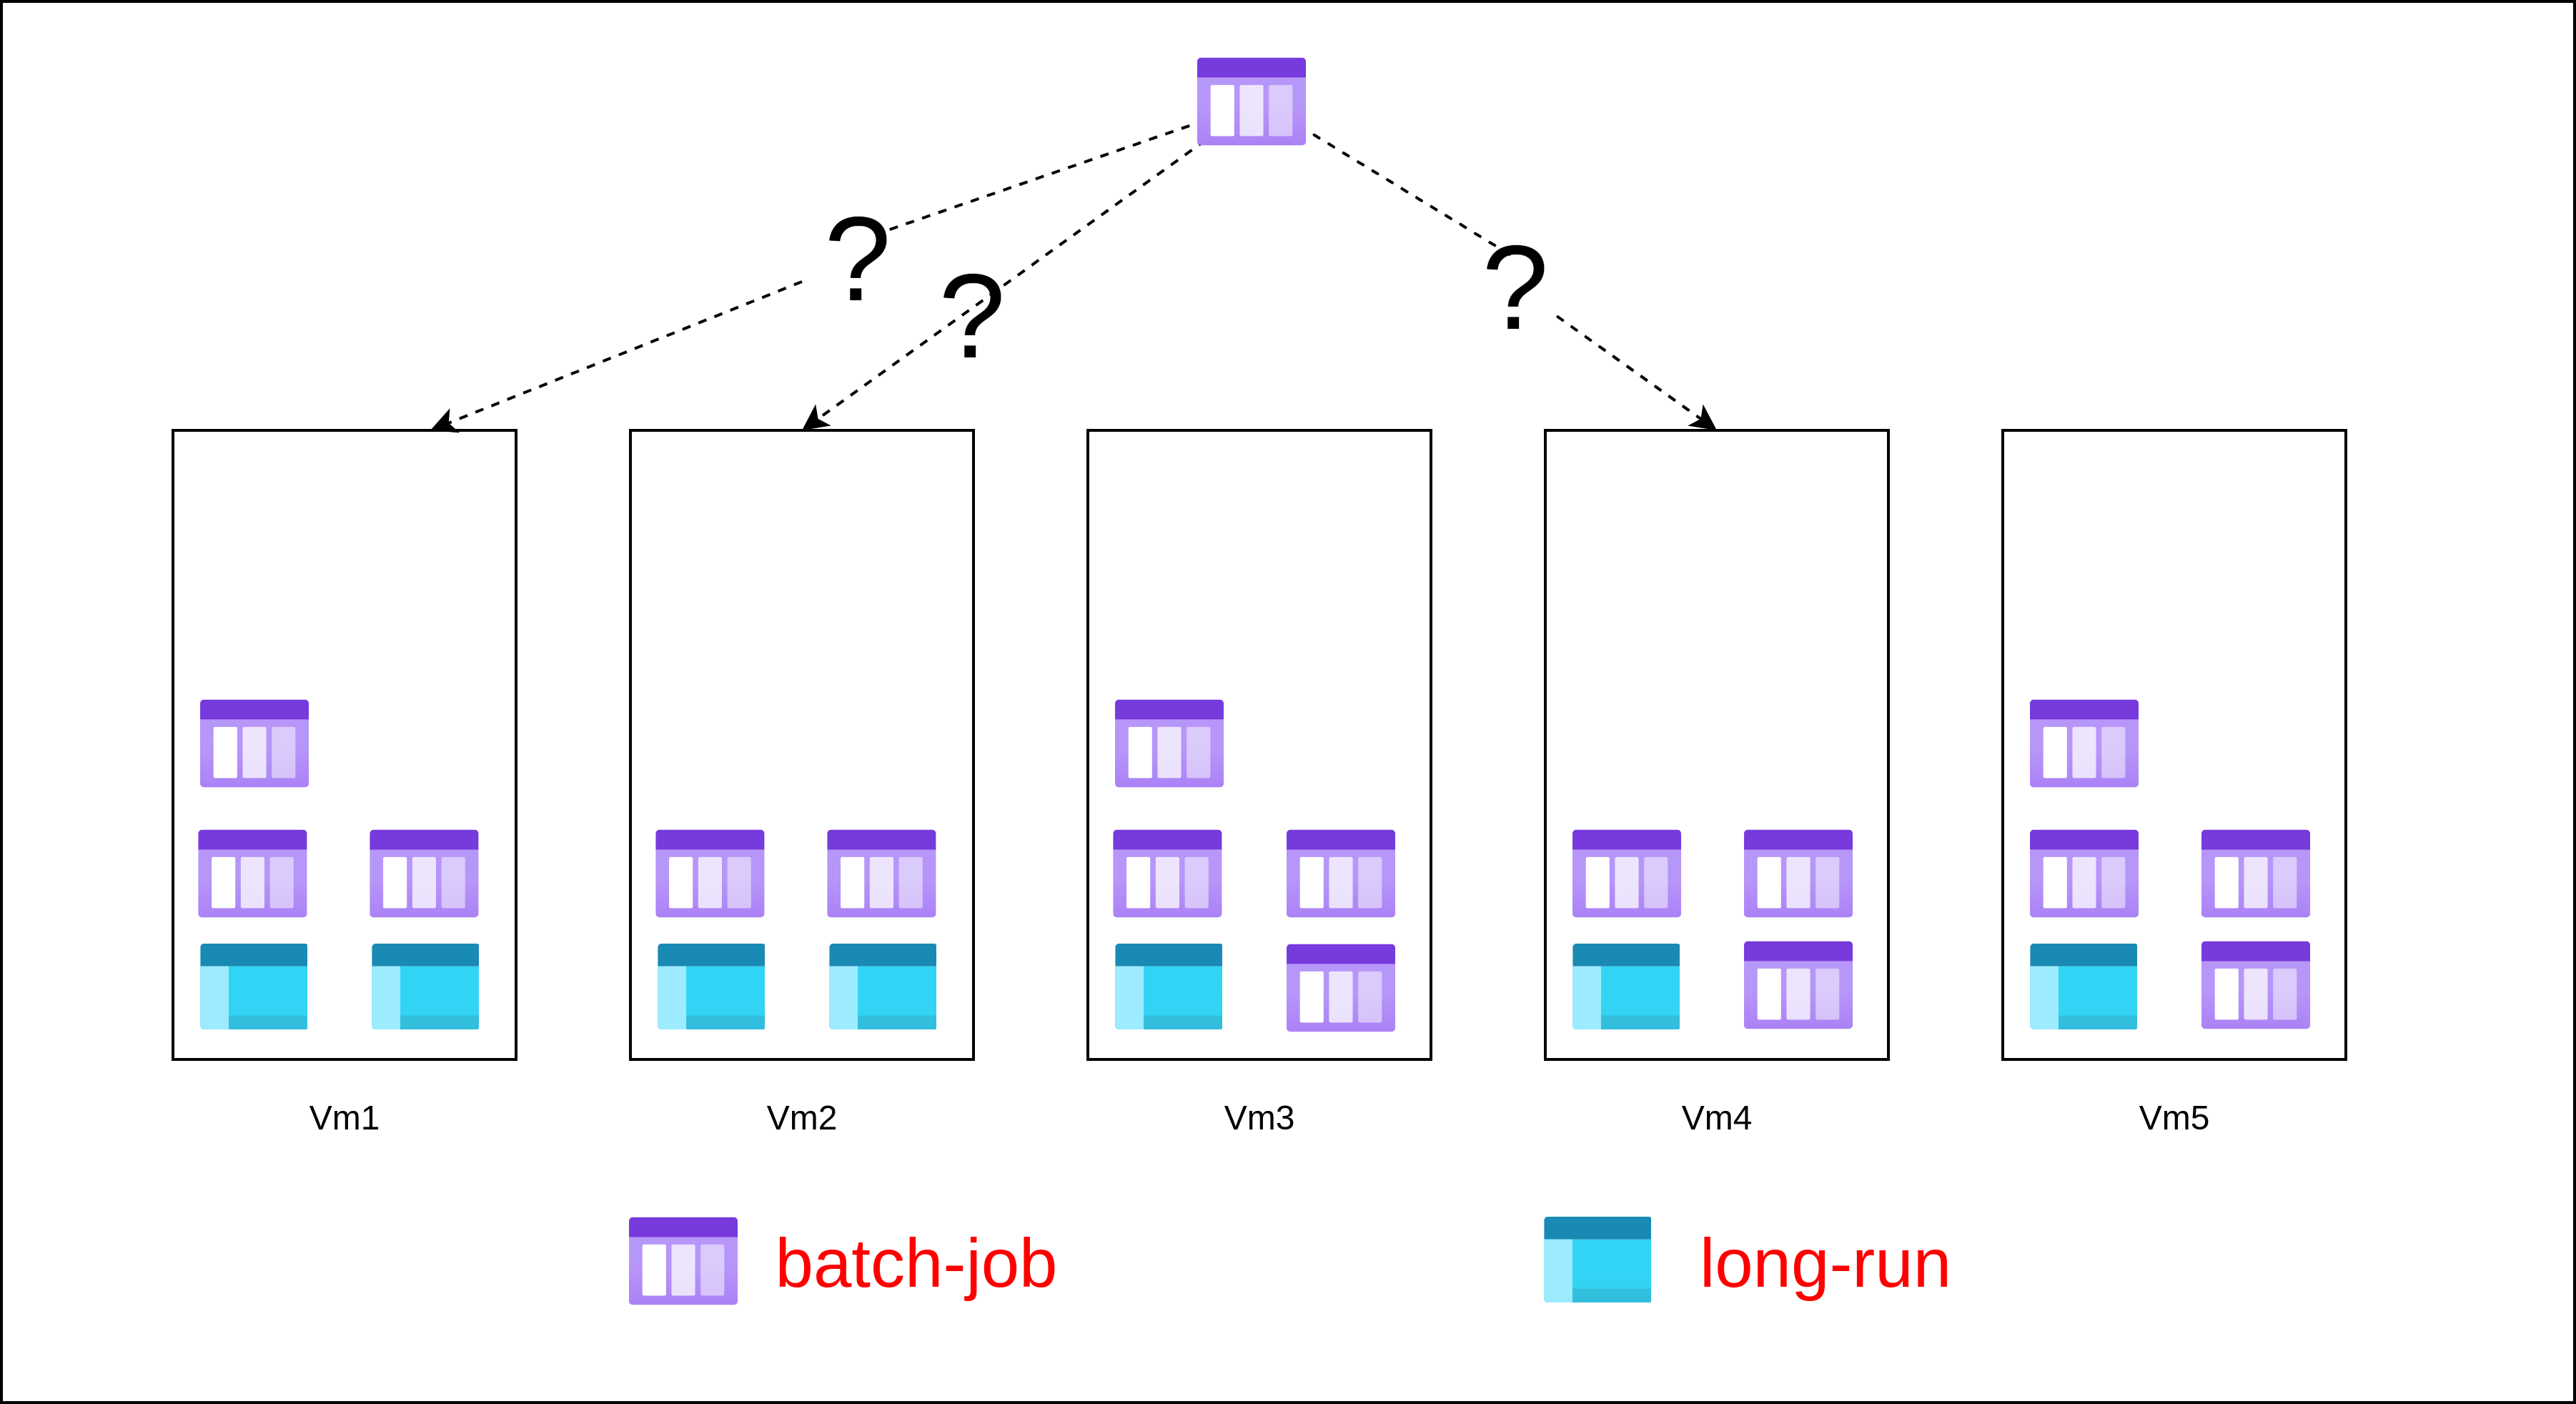
\includegraphics[scale=0.35]{images/balancing_tasks6.png}
%		\caption{Lập lịch cho tasks}
	\end{figure}
	\vspace{1cm}
	\end{minipage}
\end{frame}

\begin{frame}
{Lựa chọn máy tính ảo cho tasks}

	\begin{minipage}[t]{0.4\linewidth}
		\vspace{0.5cm}
		Tìm máy ảo cho batch-job task: 
		\begin{itemize}
			\item Bước 1: Chọn K máy ảo có lượng tài nguyên dành cho batch-job tasks nhỏ nhất 
			\item Bước 2: Trong K máy ảo tìm được, chọn máy có lượng tài nguyên khả dụng cao nhất cho task 
			\item {Bước 3}: Cập nhật thông tin task được ghép cặp với máy ảo
		\end{itemize}
	\end{minipage}
	\hfill
	\begin{minipage}[t]{0.59\linewidth}
	\begin{figure}
		\vspace{1cm}
		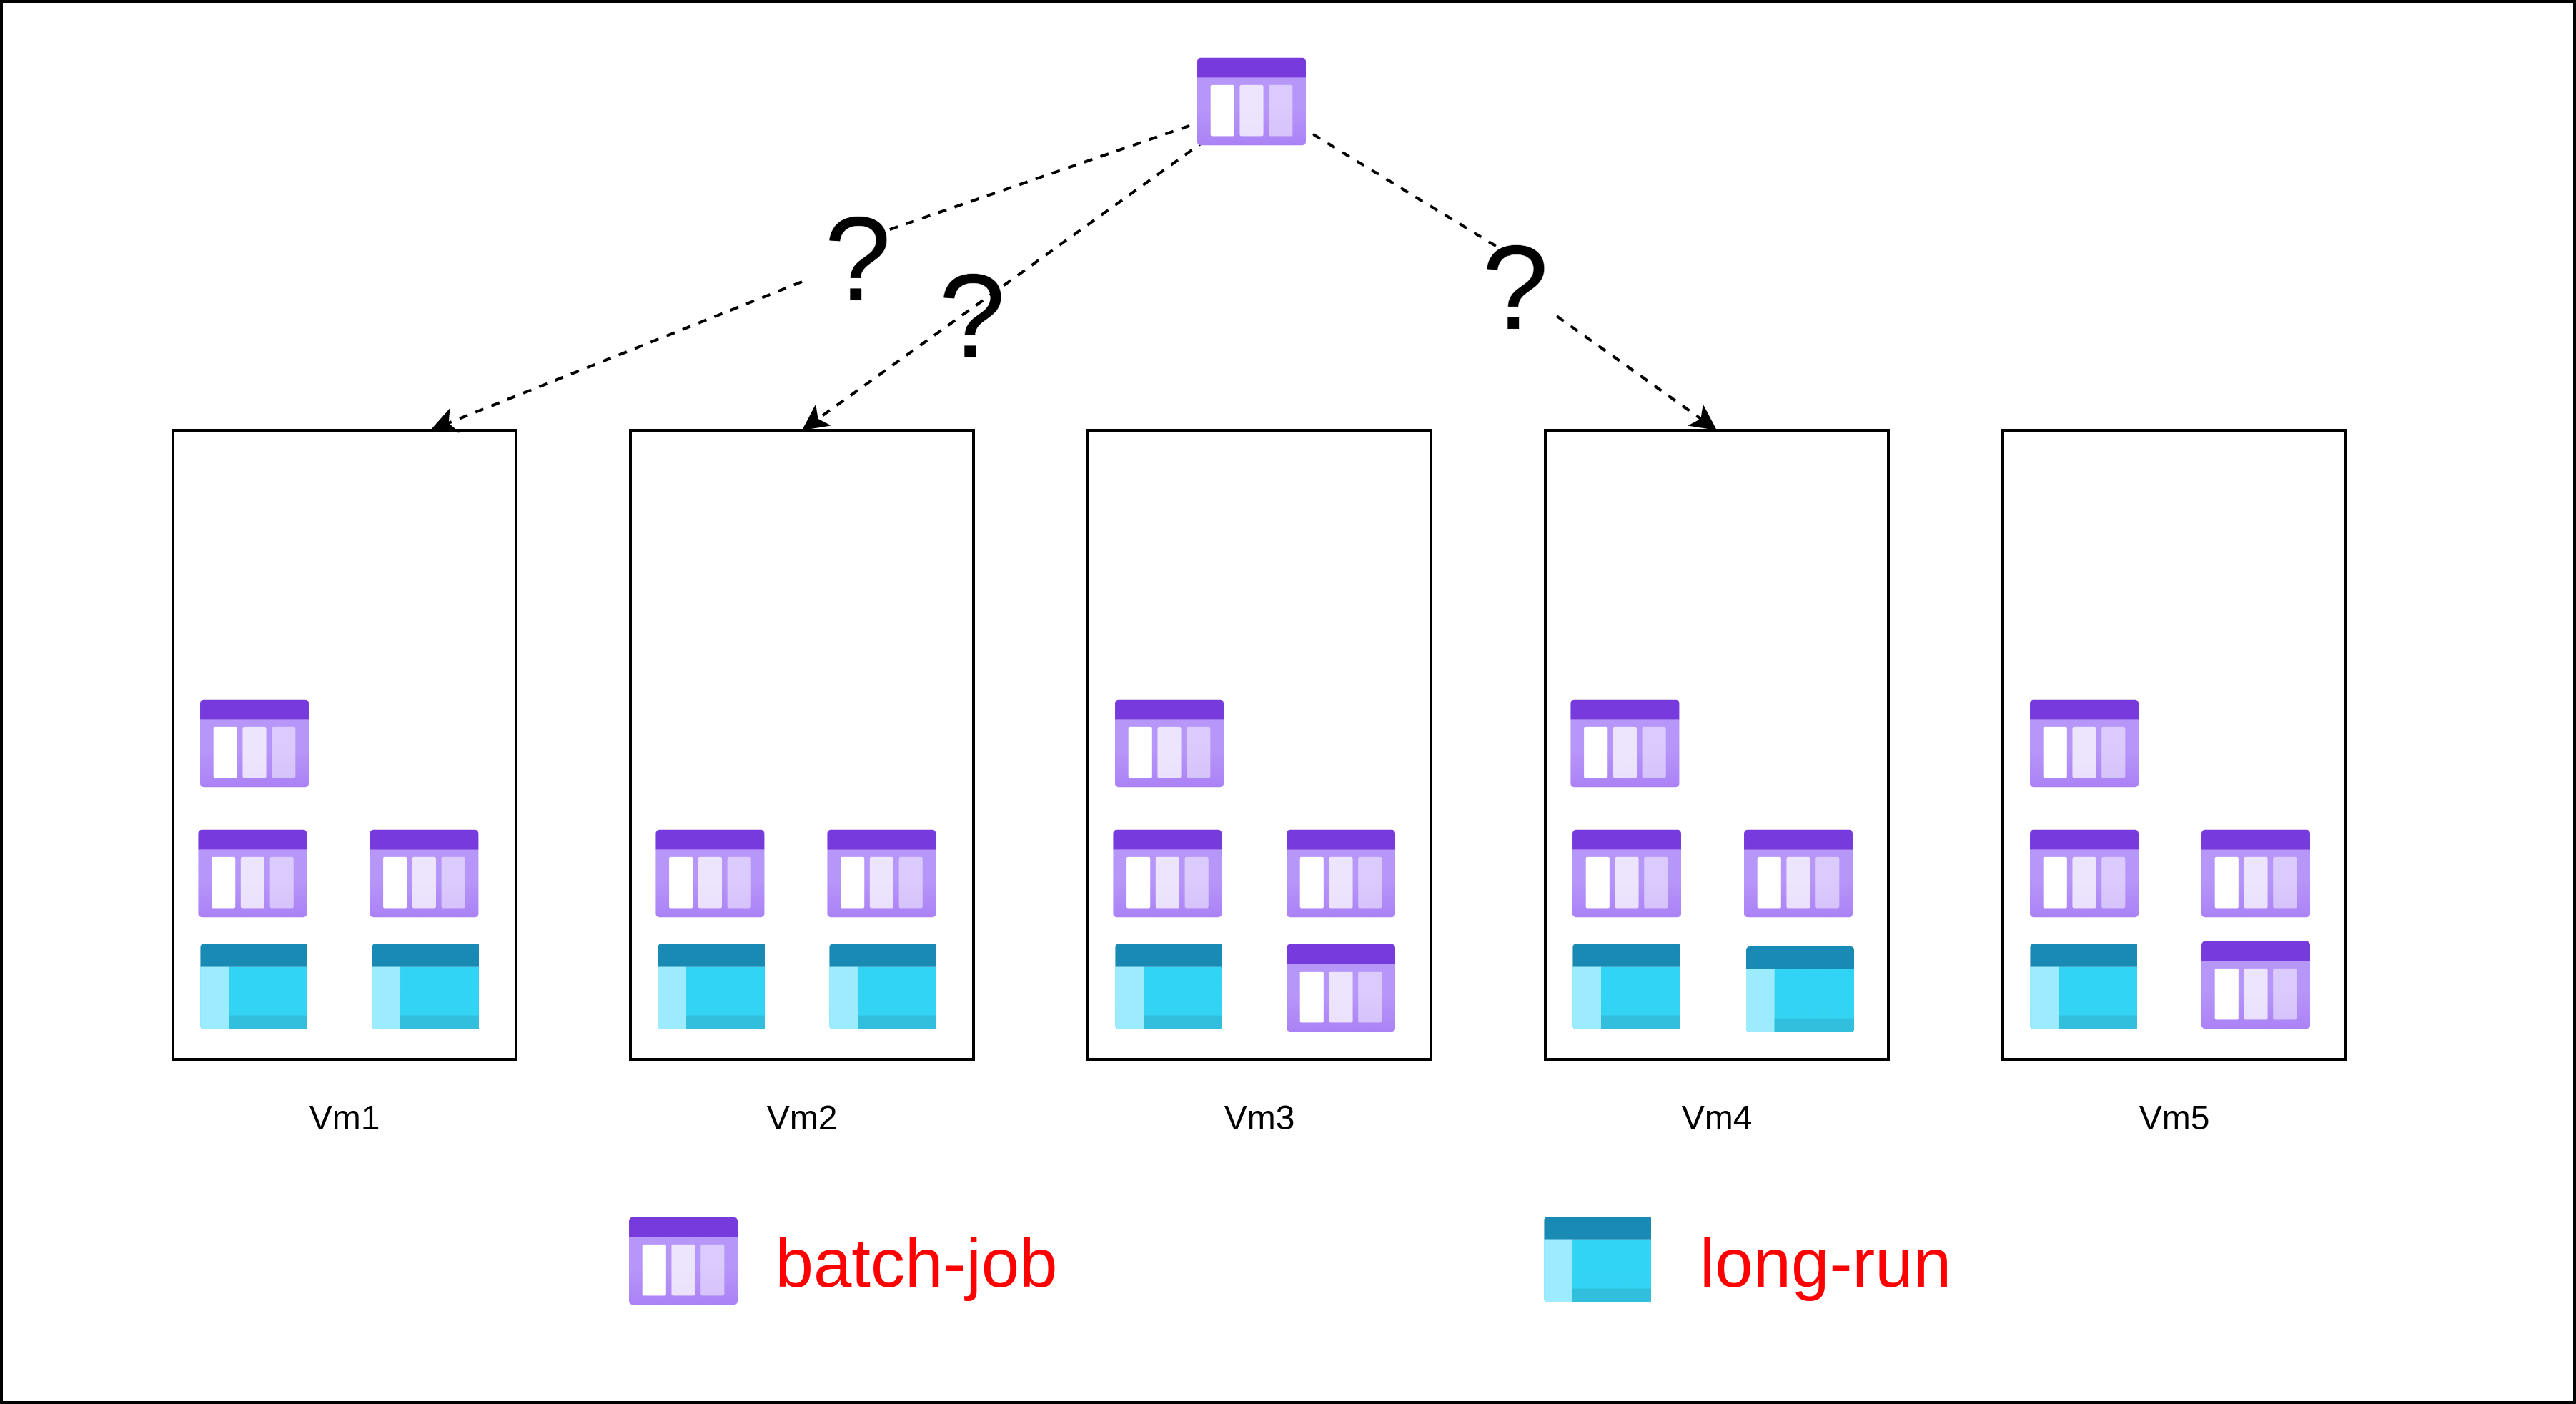
\includegraphics[scale=0.35]{images/balancing_tasks7.png}
%		\caption{Lập lịch cho tasks}
	\end{figure}
	\vspace{1cm}
	\end{minipage}
\end{frame}

\begin{frame}
{Lựa chọn máy tính ảo cho tasks}

	\begin{minipage}[t]{0.4\linewidth}
		\vspace{0.5cm}
		Tìm máy ảo cho batch-job task: 
		\begin{itemize}
			\item Bước 1: Chọn K máy ảo có lượng tài nguyên dành cho batch-job tasks nhỏ nhất 
			\item Bước 2: Trong K máy ảo tìm được, chọn máy có lượng tài nguyên khả dụng cao nhất cho task 
			\item {Bước 3}: Cập nhật thông tin task được ghép cặp với máy ảo
		\end{itemize}
	\end{minipage}
	\hfill
	\begin{minipage}[t]{0.59\linewidth}
	\begin{figure}
		\vspace{1cm}
		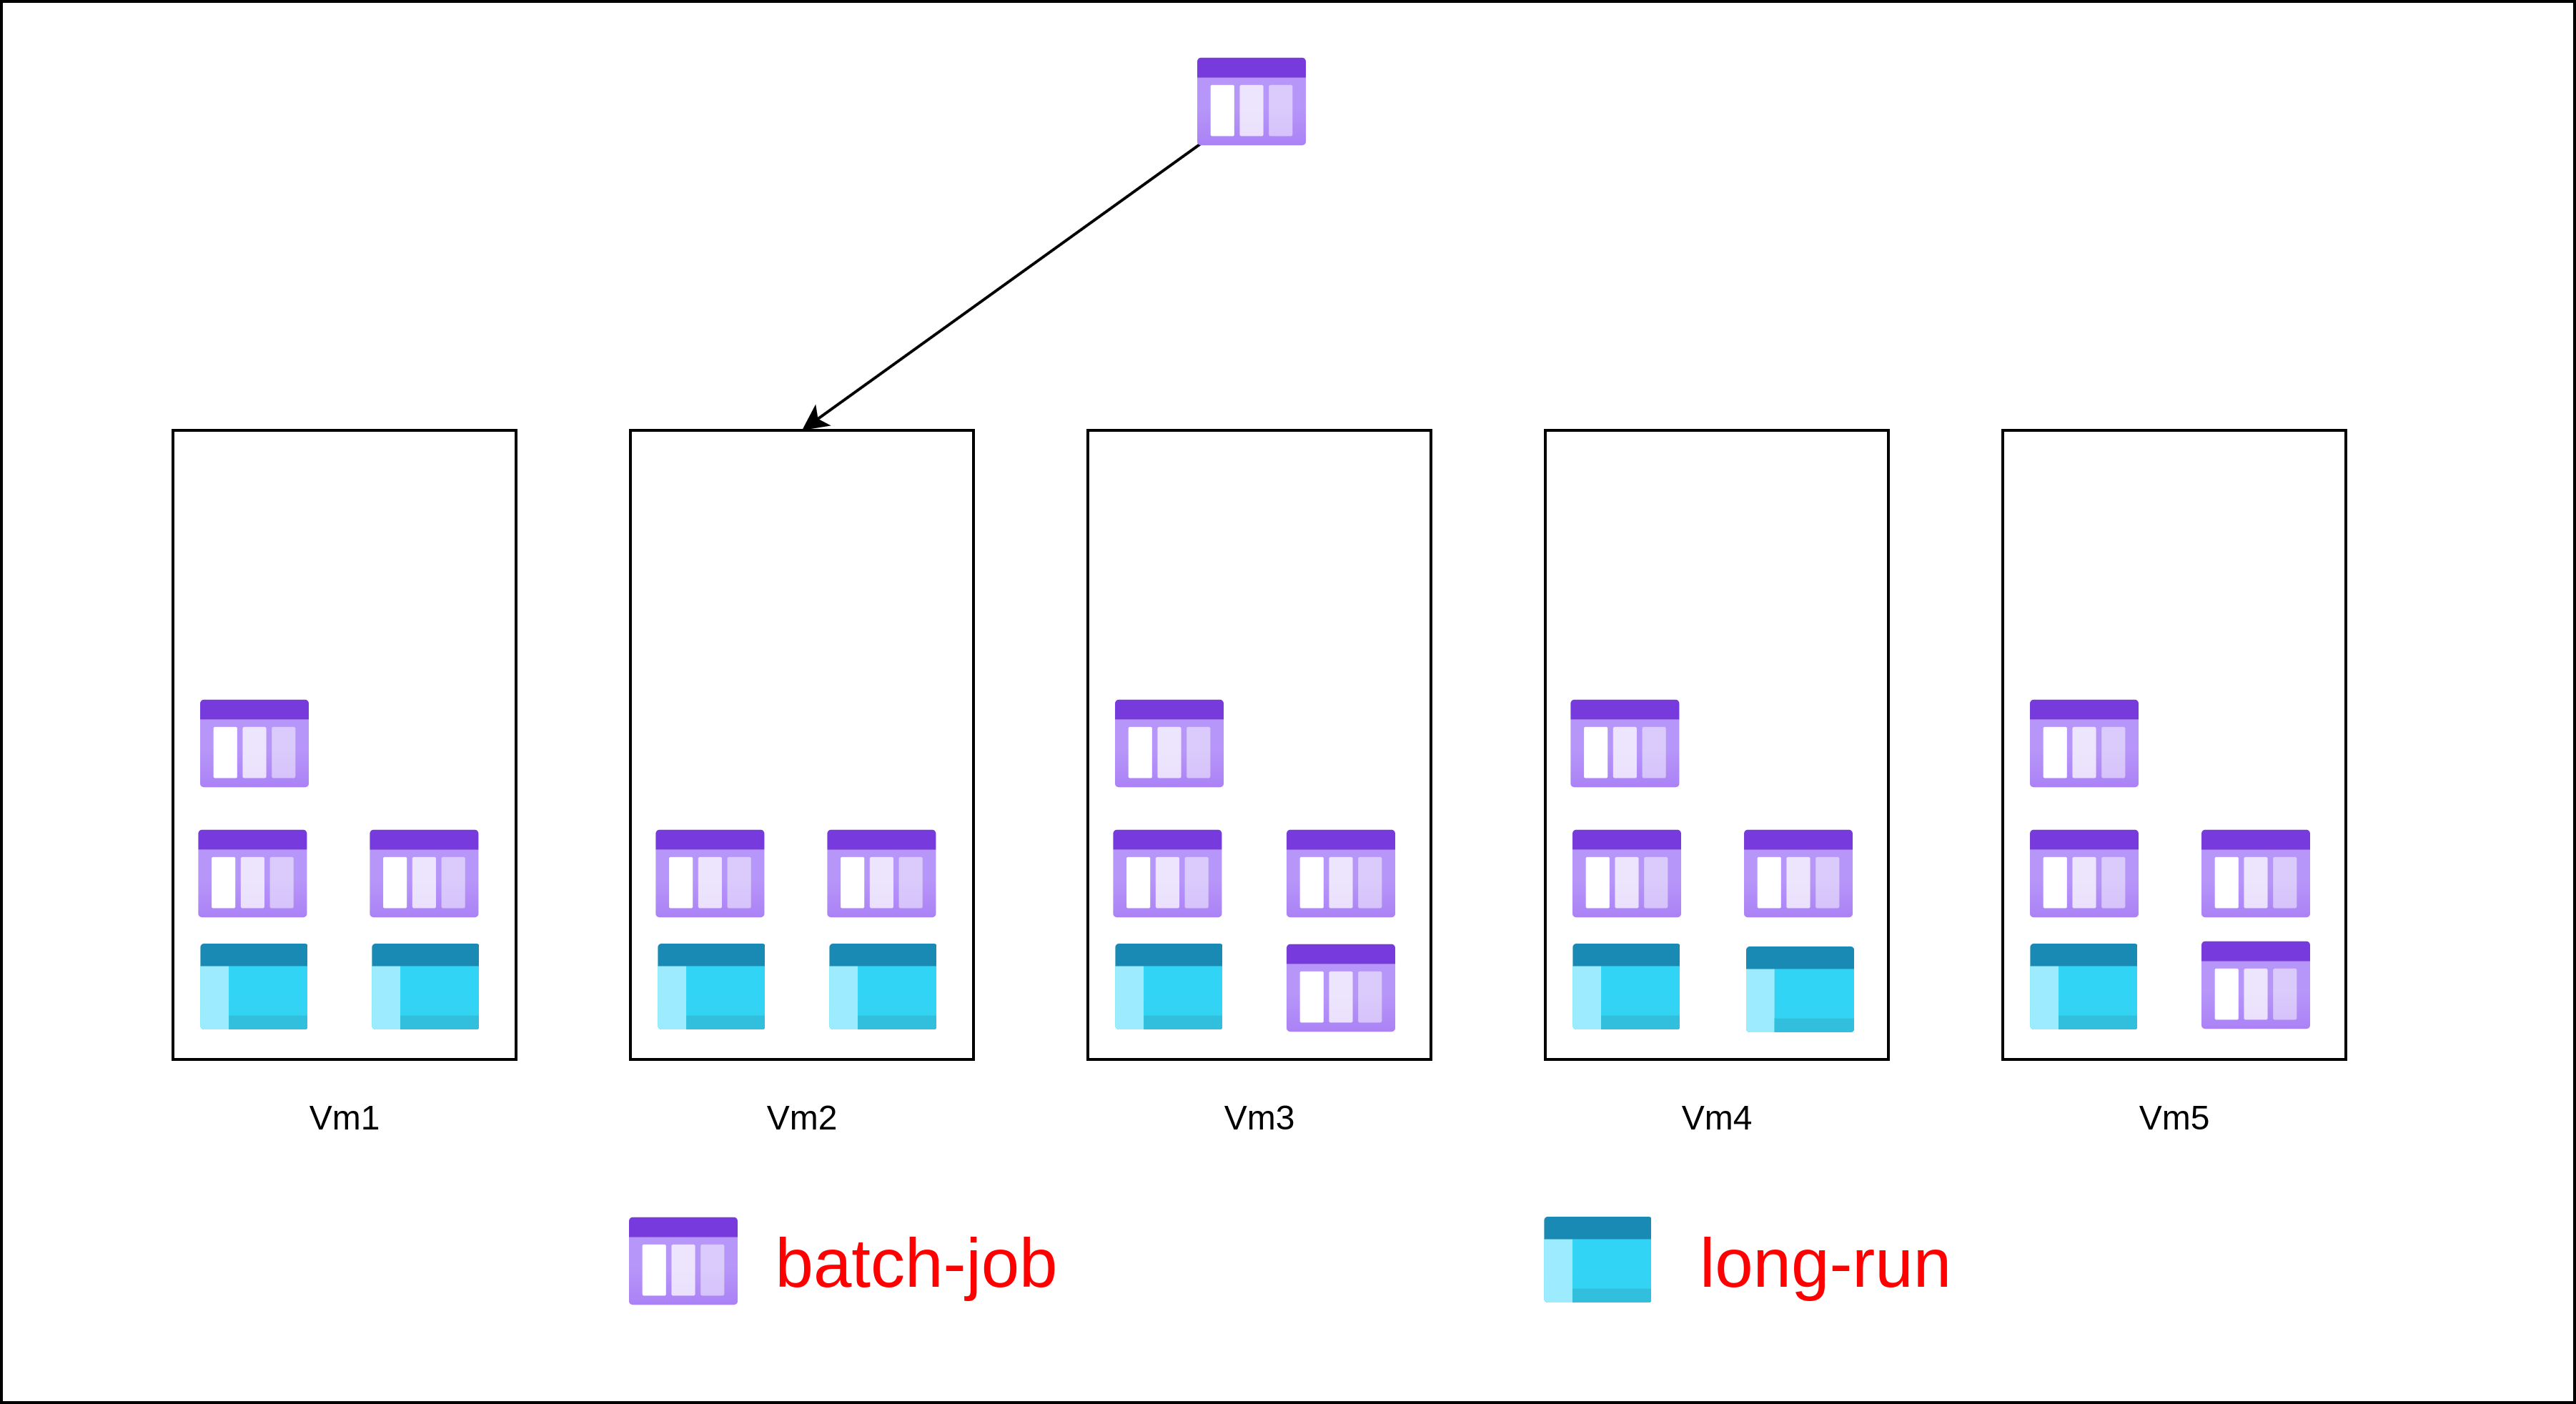
\includegraphics[scale=0.35]{images/balancing_tasks8.png}
%		\caption{Lập lịch cho tasks}
	\end{figure}
	\vspace{1cm}
	\end{minipage}
\end{frame}

\begin{frame}
{Lựa chọn máy tính ảo cho tasks}

	\begin{minipage}[t]{0.4\linewidth}
		\vspace{0.5cm}
		Tìm máy ảo cho batch-job task: 
		\begin{itemize}
			\item Bước 1: Chọn K máy ảo có lượng tài nguyên dành cho batch-job tasks nhỏ nhất 
			\item Bước 2: Trong K máy ảo tìm được, chọn máy có lượng tài nguyên khả dụng cao nhất cho task 
			\item {Bước 3}: Cập nhật thông tin task được ghép cặp với máy ảo
		\end{itemize}
	\end{minipage}
	\hfill
	\begin{minipage}[t]{0.59\linewidth}
	\begin{figure}
		\vspace{1cm}
		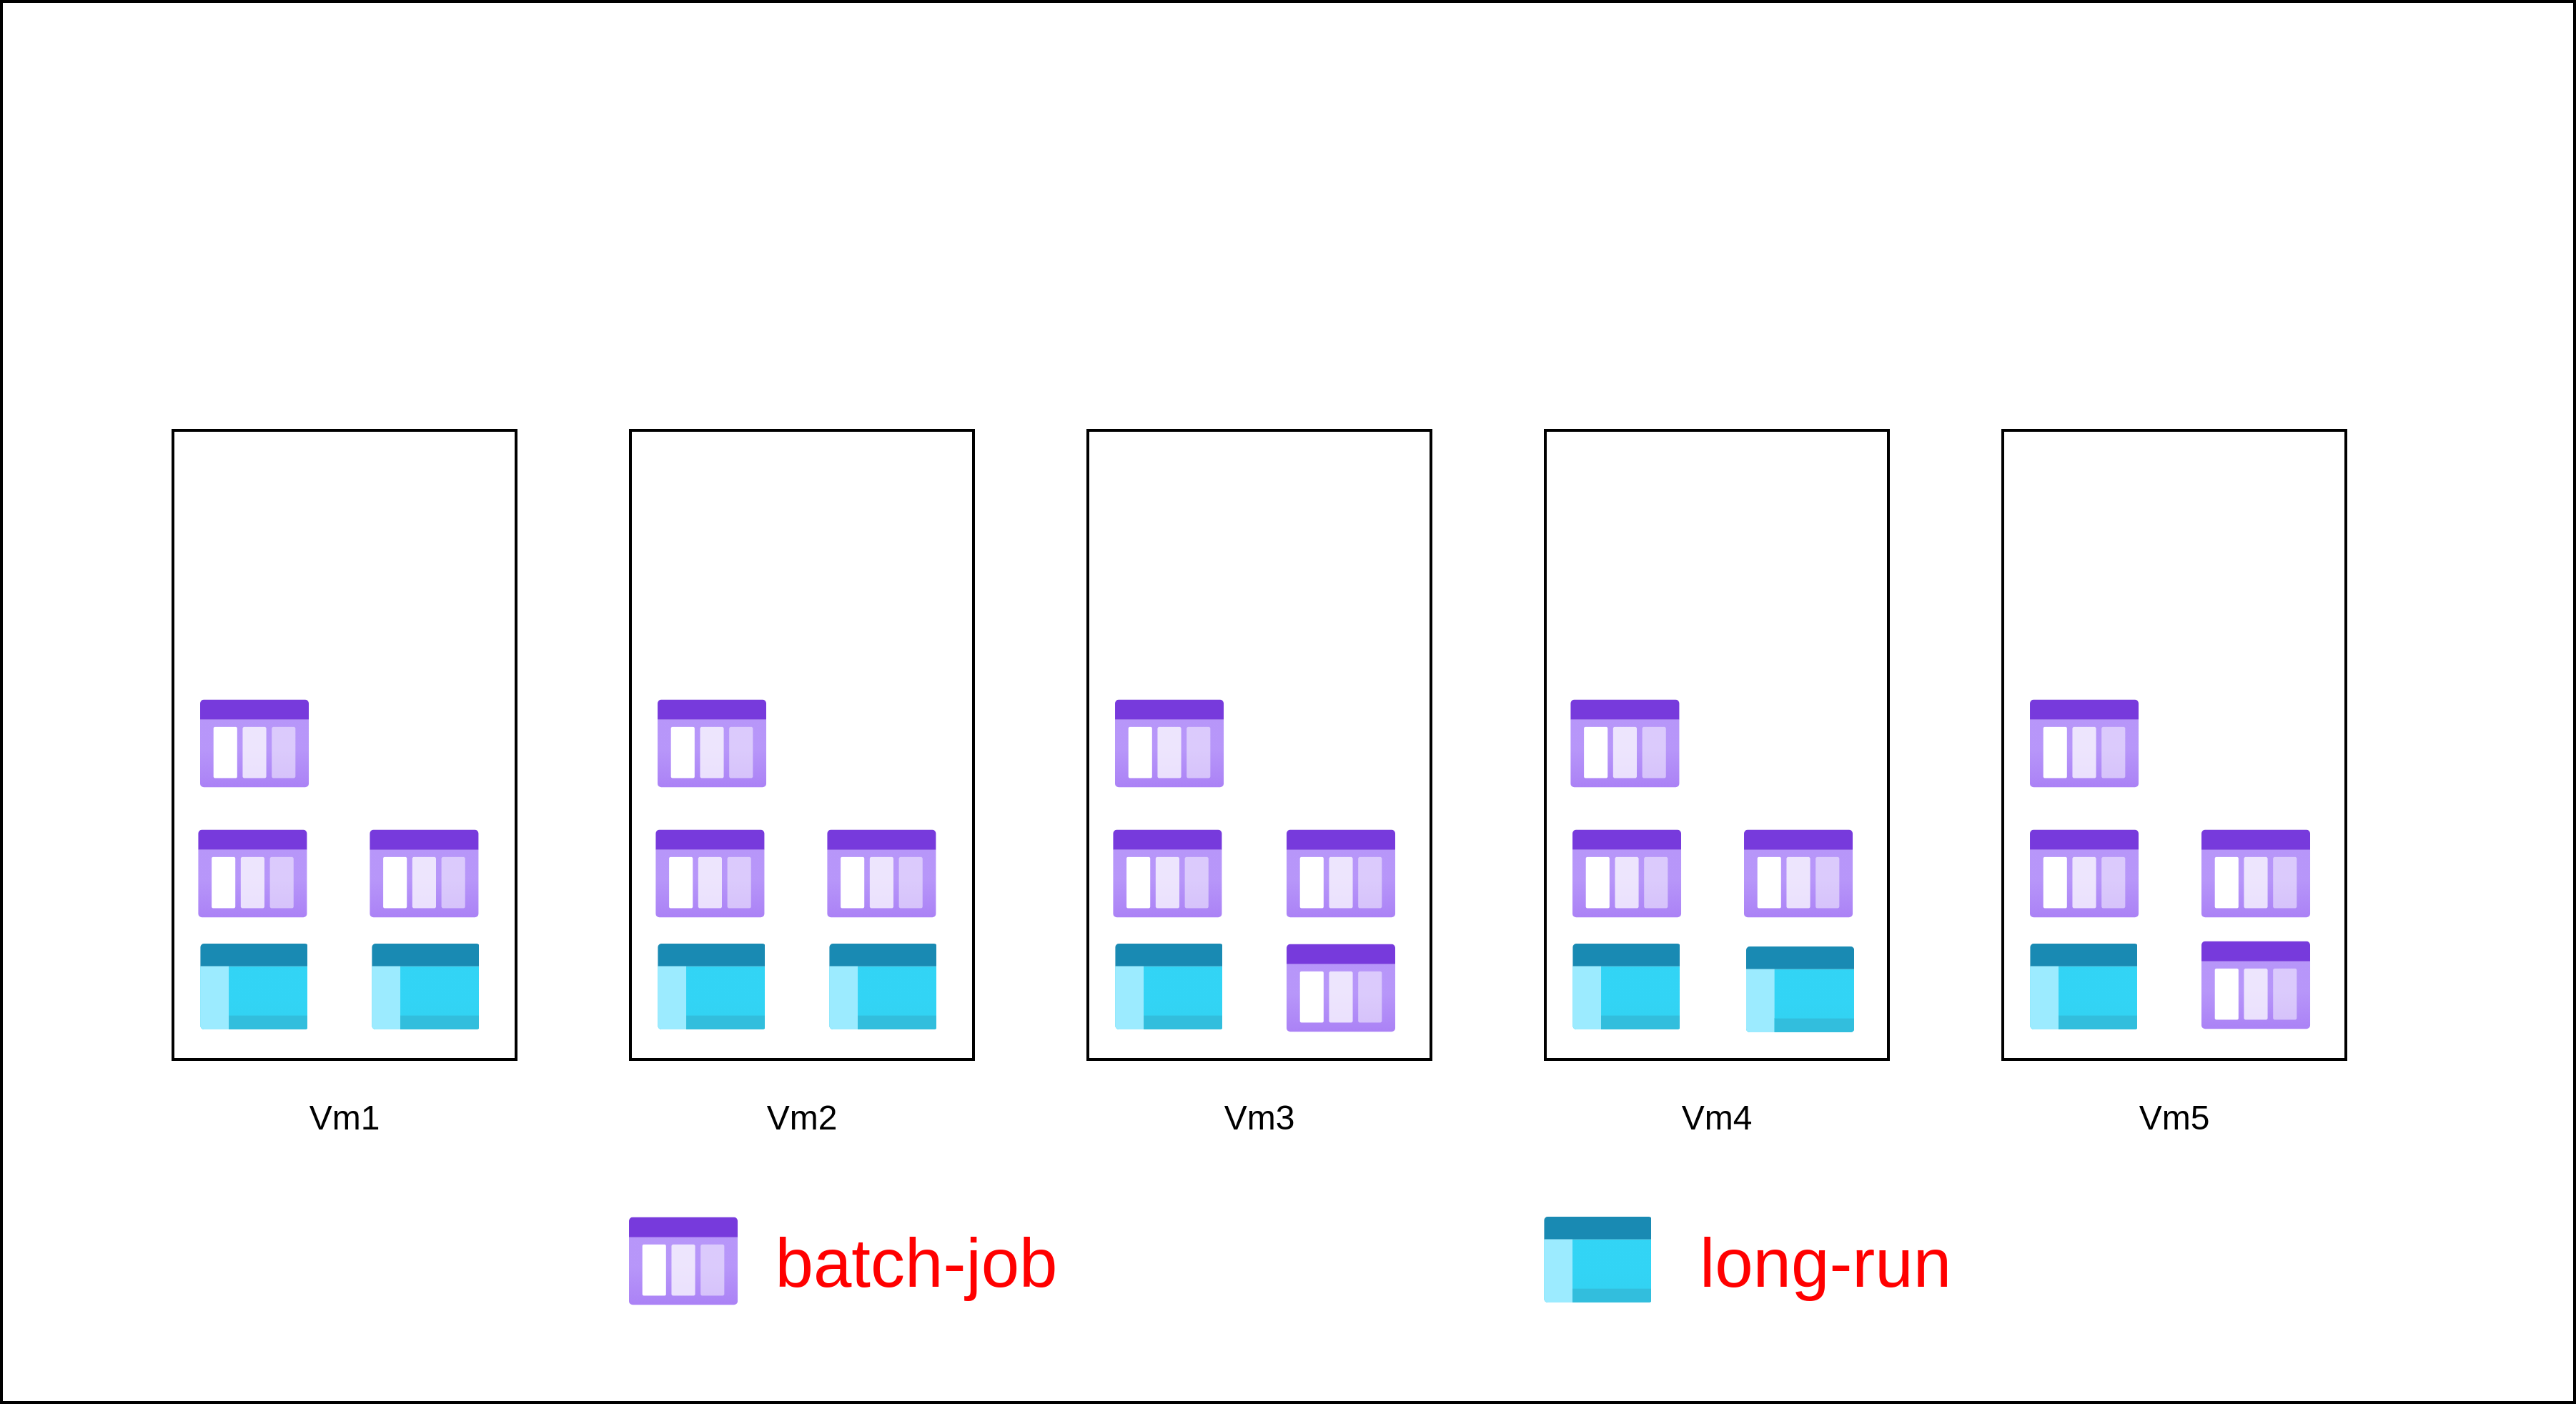
\includegraphics[scale=0.35]{images/balancing_tasks9.png}
%		\caption{Lập lịch cho tasks}
	\end{figure}
	\vspace{1cm}
	\end{minipage}
\end{frame}

\begin{frame}
{Mô hình lập lịch đề xuất}
	\begin{minipage}[t]{0.39\linewidth}
		\vspace{2cm}
		\begin{itemize}
			\item Dùng mạng Bayesian ước lượng tài nguyên khả dụng 
			\item \textbf{Dùng tài nguyên ước lượng để lập lịch cho tasks}
		\end{itemize}
	\end{minipage}
	\hfill
	\begin{minipage}[t]{0.6\linewidth}
	\vspace{0.5cm}
		\begin{figure}
			\centering
			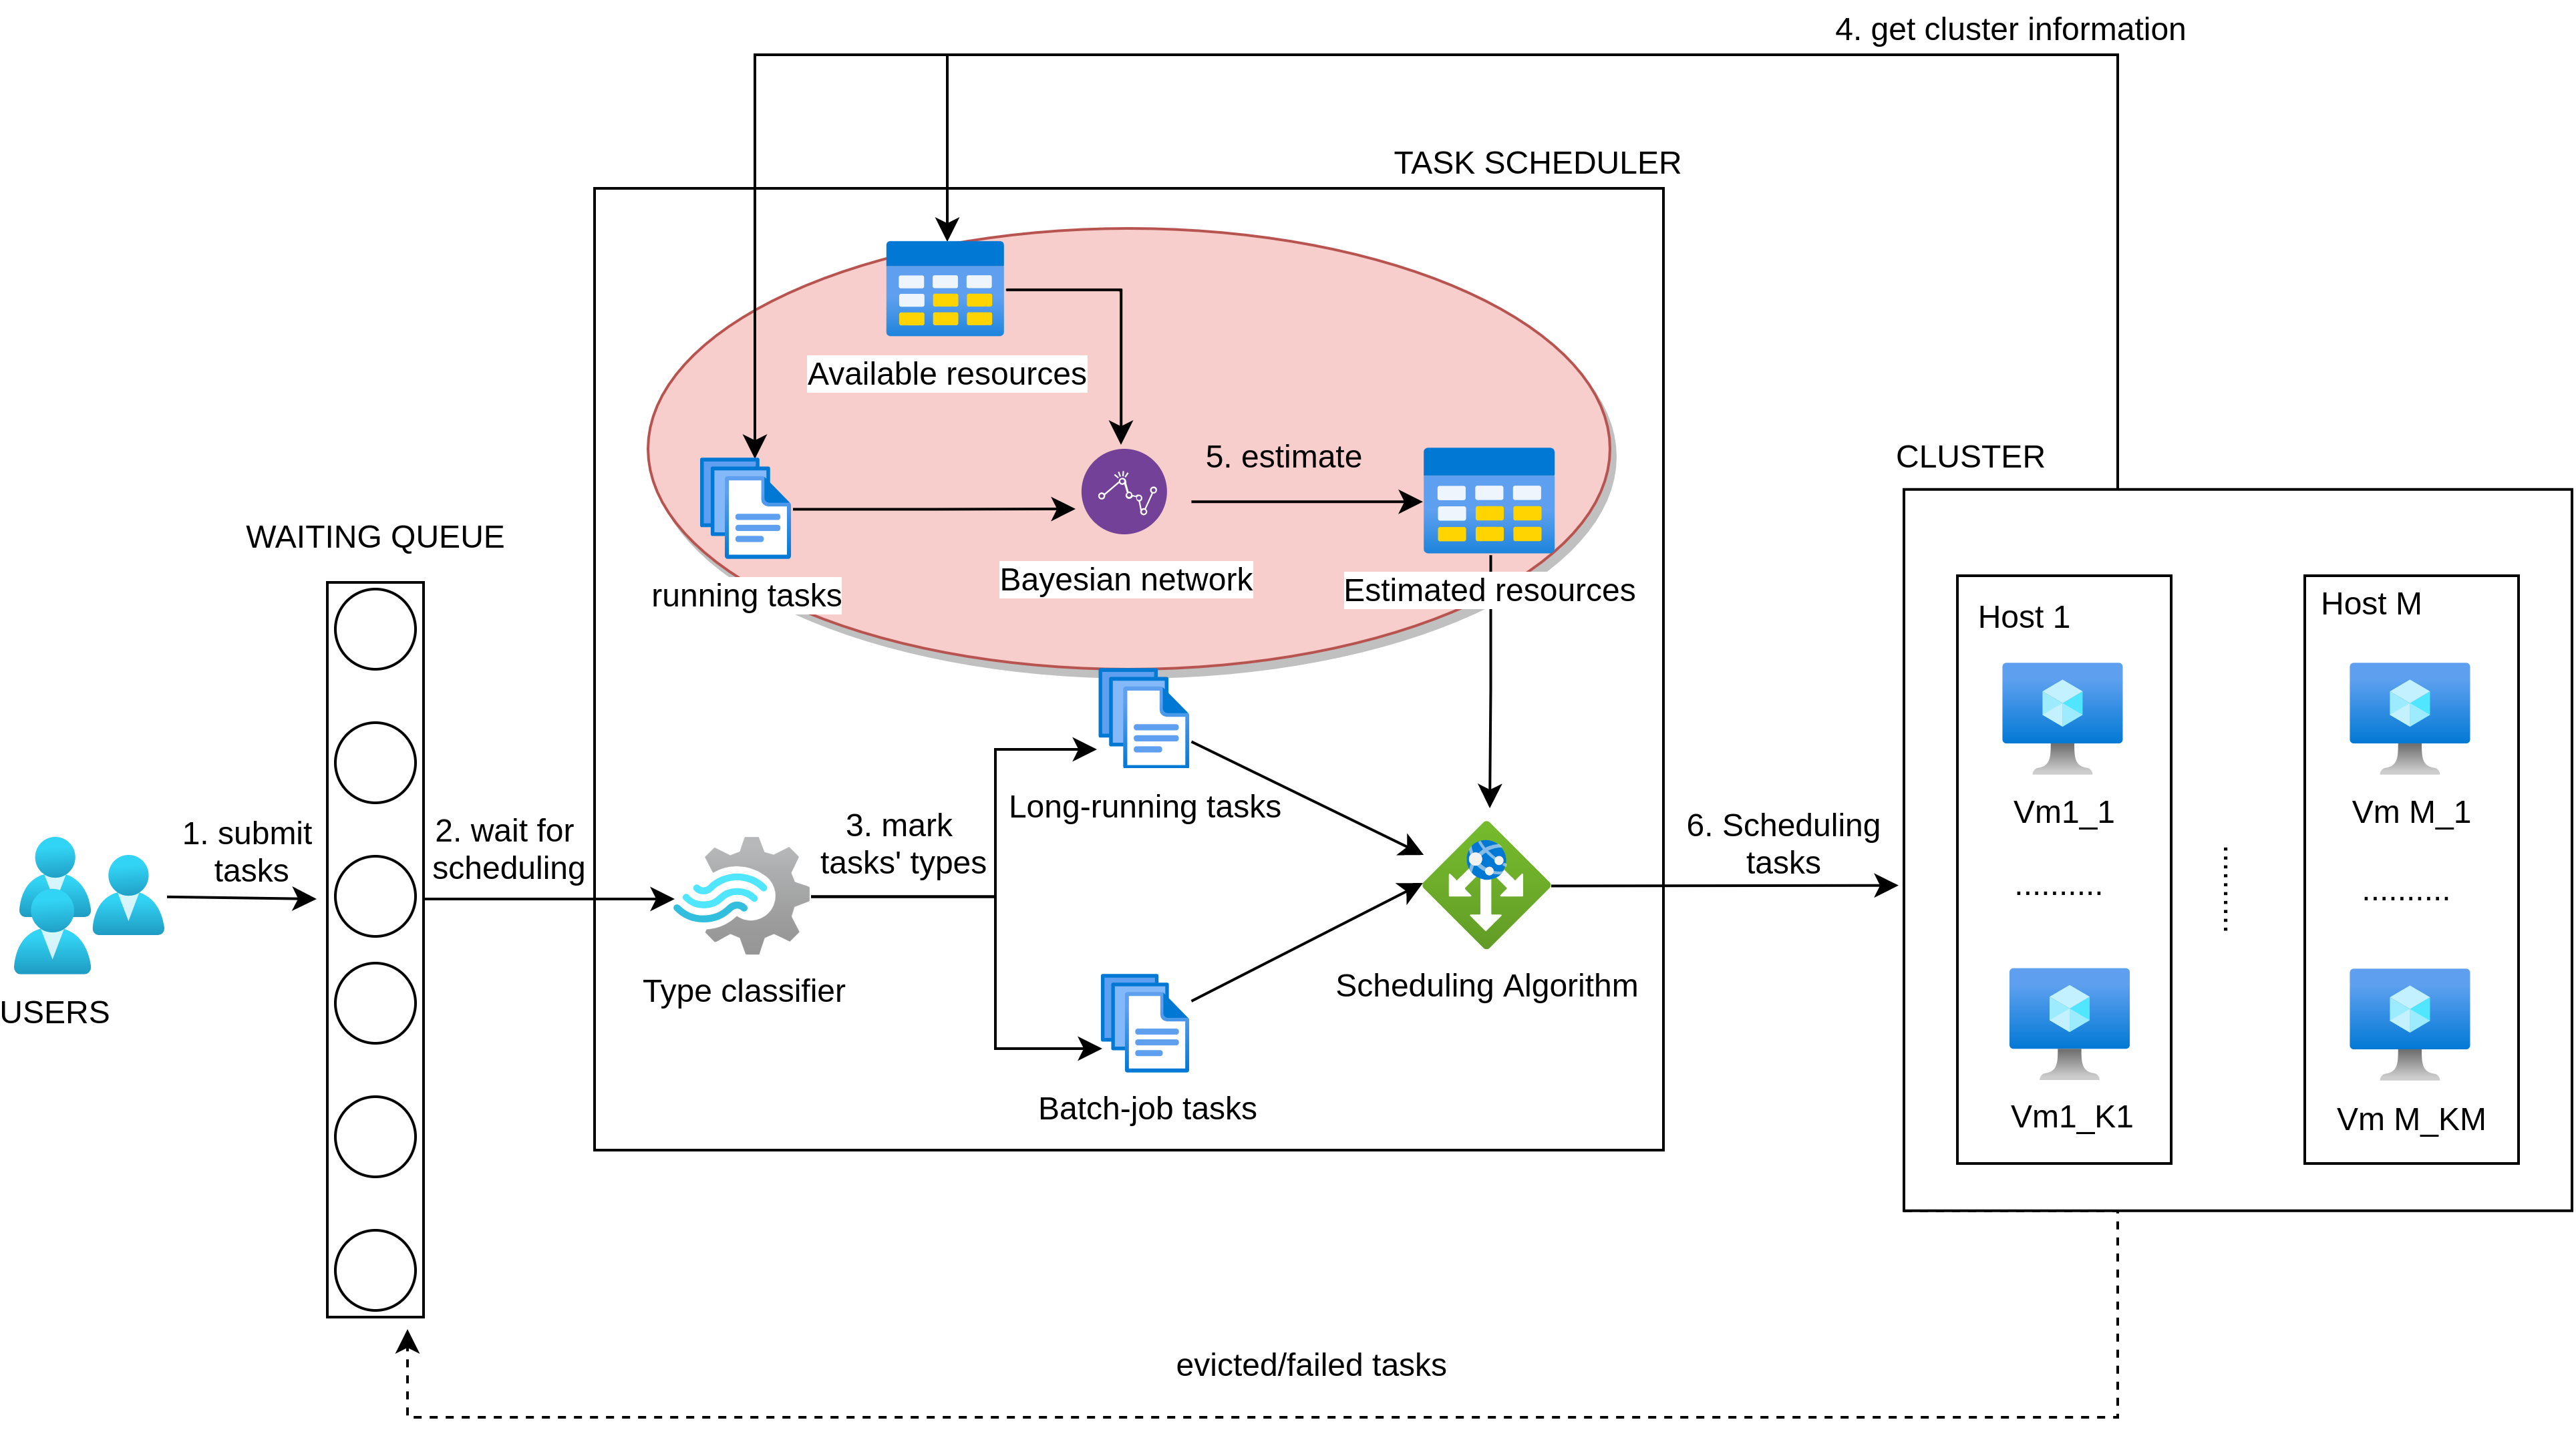
\includegraphics[scale=0.35]{images/bayesian_application.png}		
		\end{figure}			
	\end{minipage}
\end{frame}

\section{Đánh giá hiệu năng} 

\begin{frame}
{Thực nghiệm}
% Mô tả dữ liệu mô phỏng 

\begin{block}
{Mục đích}
	\begin{enumerate}
		\item Đánh giá hiệu năng so với Worstfit và FCFS
		\item Đánh giá hiệu quả của mạng Bayesian
		\item So sánh độ mất cân bằng trong thời gian chạy với Worstfit	
	\end{enumerate}
\end{block}

\begin{block}
{Kịch bản}
\begin{itemize}
	\item M = 10 máy tính ảo 
	\item N = 15000 tasks
	\item K = 3
	\item $T \sim \mathcal{P}(\lambda = 15)$
	\item $delay\_time \sim \mathcal{N}(\mu = 5, \sigma = 0.5^{2})$
\end{itemize}
\end{block}

\end{frame}

\begin{frame}
{Số liệu so sánh về thời gian}

	\begin{minipage}[t]{0.4\linewidth}
		\vspace{1.5cm}
		\begin{itemize}
			\item Thuật toán đề xuất hoàn thành nhiều tasks hơn so với Worstfit và FCFS
			\item Thời gian trung bình hoàn thành một task tốt hơn FCFS là 50\%, Worstfit là 20\%
		\end{itemize}
	\end{minipage}
	\hfill
	\begin{minipage}[t]{0.59\linewidth}
\begin{table}[h!]
	\centering
	\caption{Kết quả về thời gian chạy của các tasks}
	\begin{tabular}{|p{1.5cm}| p{1.5cm} | p{1.5cm} | p{1.6cm}|}
		\hline
		\multicolumn{4}{|c|}{Running statistics over 1000s} \\
		\hline
		stats & FCFS & Worstfit & Resources \\
			&	&	& balancing \\
		\hline
		\hline
		count&\color{red}{13214}&\color{red}{13925}&\color{red}{14235} \\
		\hline
		mean&\color{blue}10.62&\color{blue}{6.34}&\color{blue}{5.42}\\
		\hline
		std&54.24&33.37&27.31 \\
		\hline
		min&0.31&0.12&0.21 \\
%		\hline
%		25\%&3.15&2.09&2.08 \\
		\hline
		50\%&5.78&3.52&3.41 \\
%		\hline
%		75\%&8.13&5.61&5.50 \\
		\hline
		max&829.92&616.35&640.39 \\
		\hline
	\end{tabular}
	\label{table:finished_tasks}
\end{table}
	\end{minipage}
\end{frame}

\begin{frame}
{So sánh độ chính xác của mạng Bayesian}
\begin{figure}
\centering
\begin{subfigure}{.5\textwidth}
  \centering
  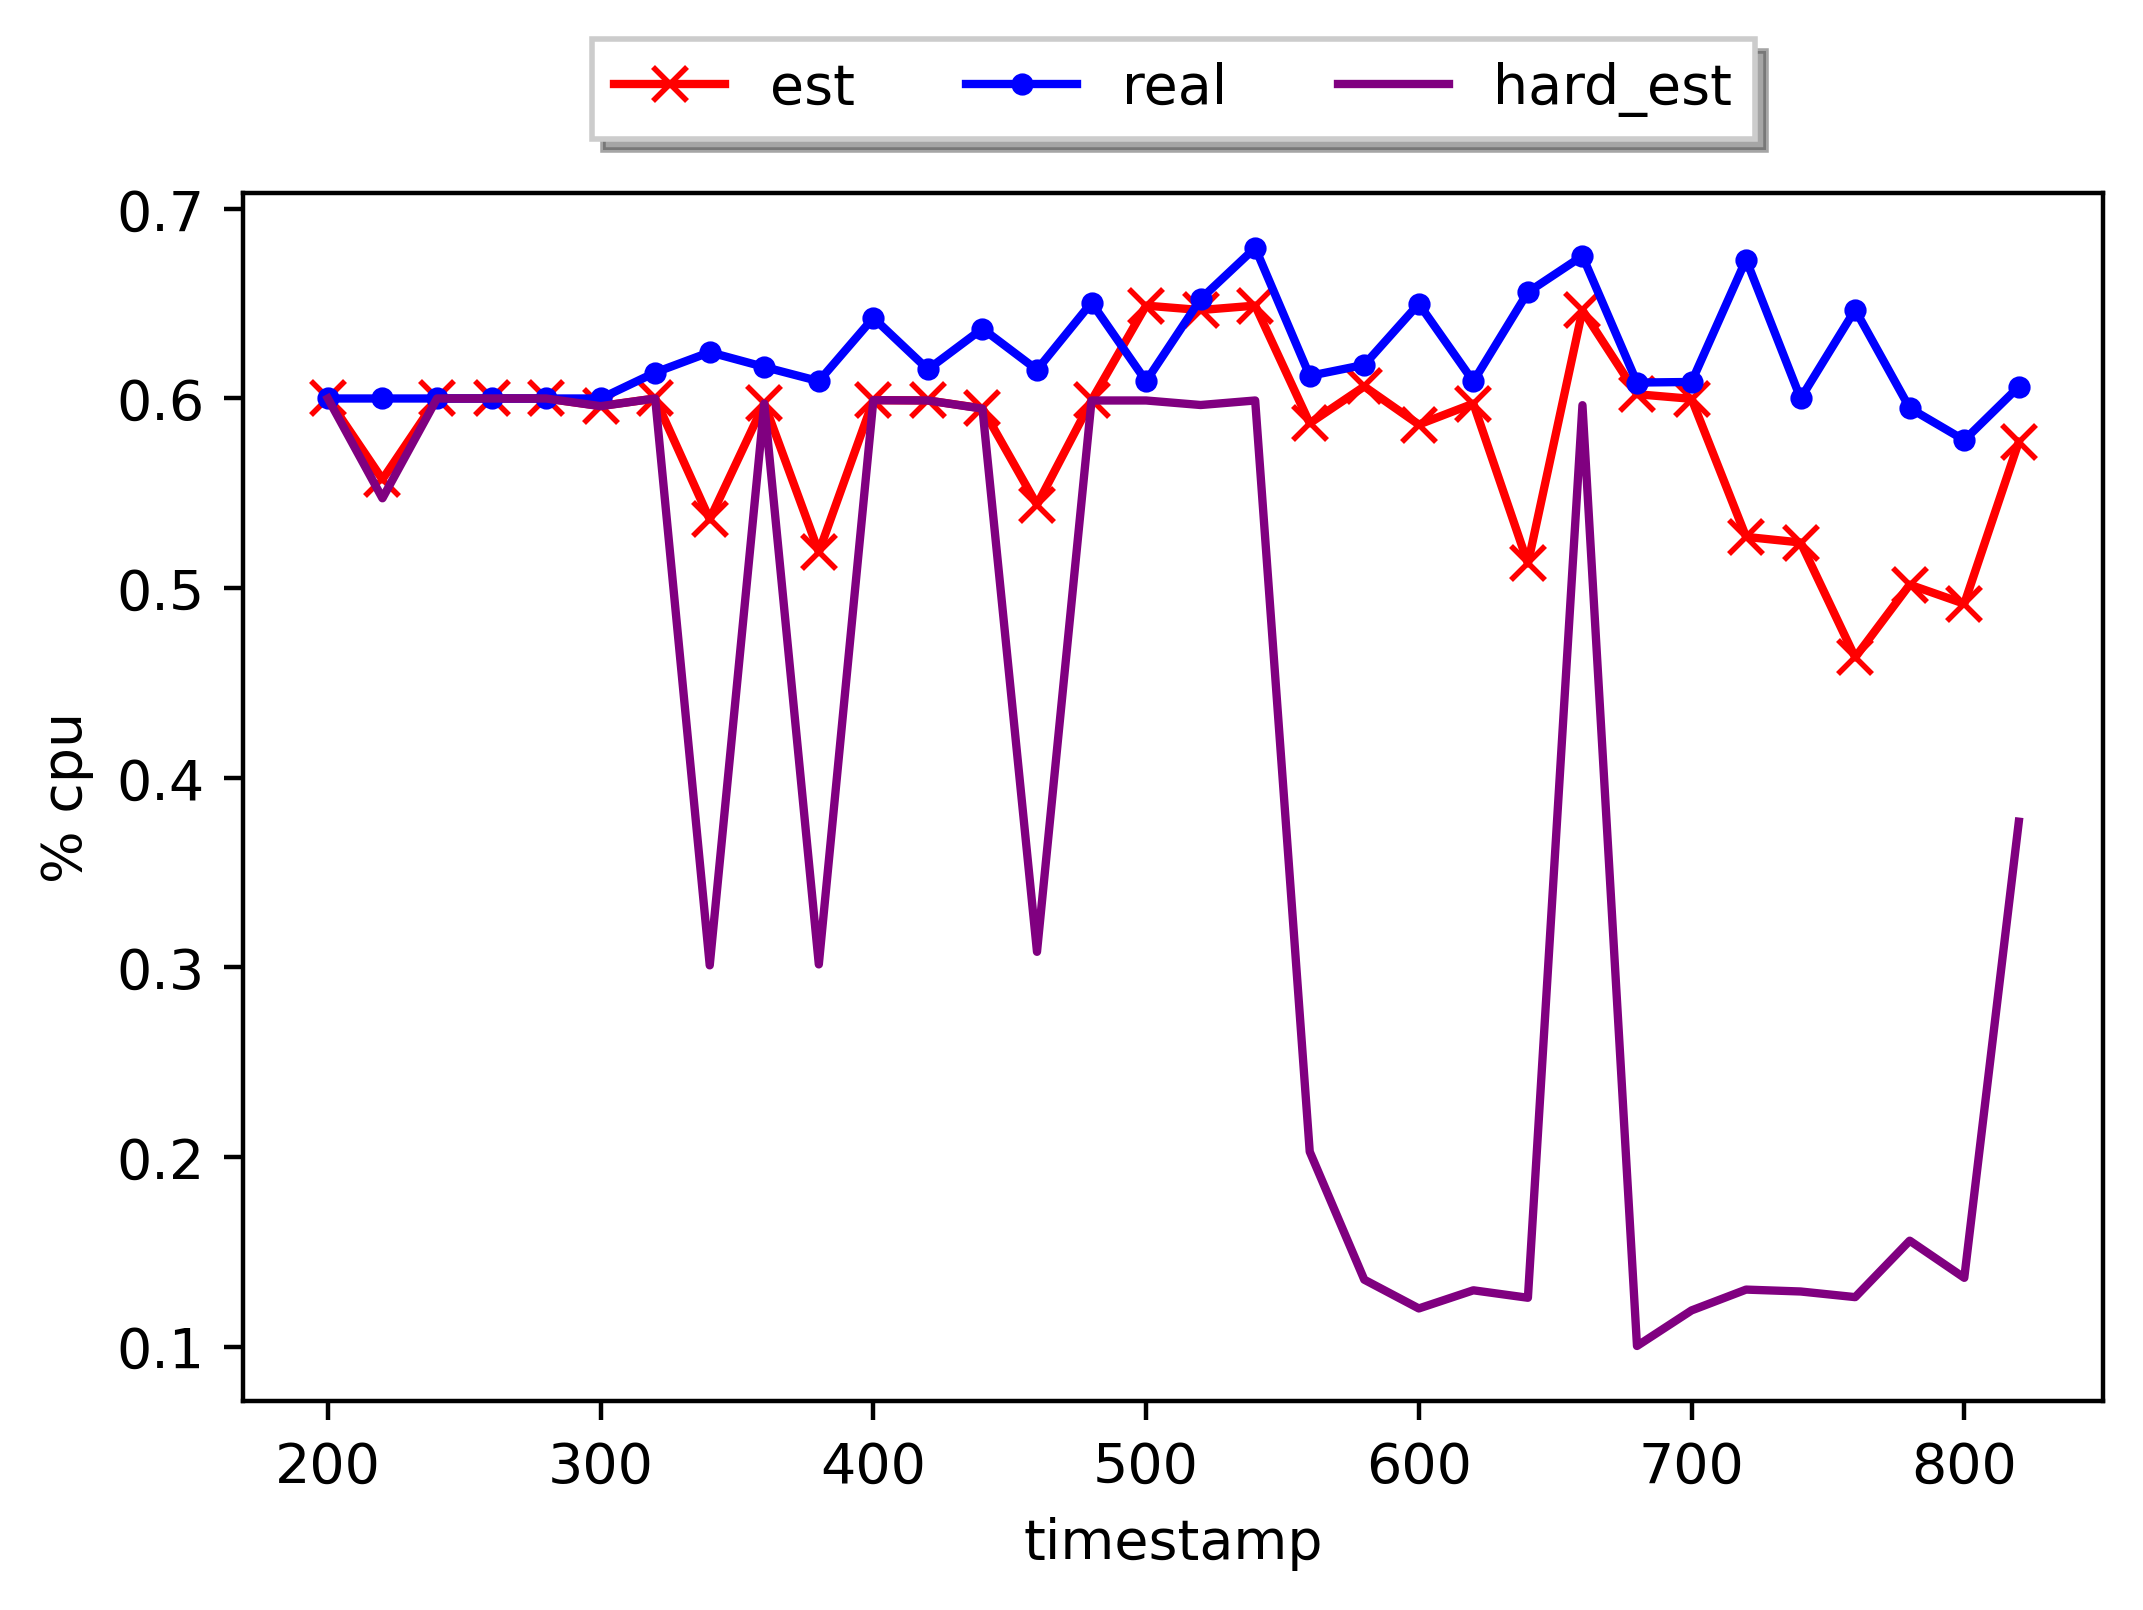
\includegraphics[width=.75\linewidth]{images/cpu_usage_estimation_1.png}
  \caption{Tài nguyên khả dụng tại thời điểm thực thi}
  \label{fig:usage_est_a}
\end{subfigure}%
\begin{subfigure}{.5\textwidth}
  \centering
  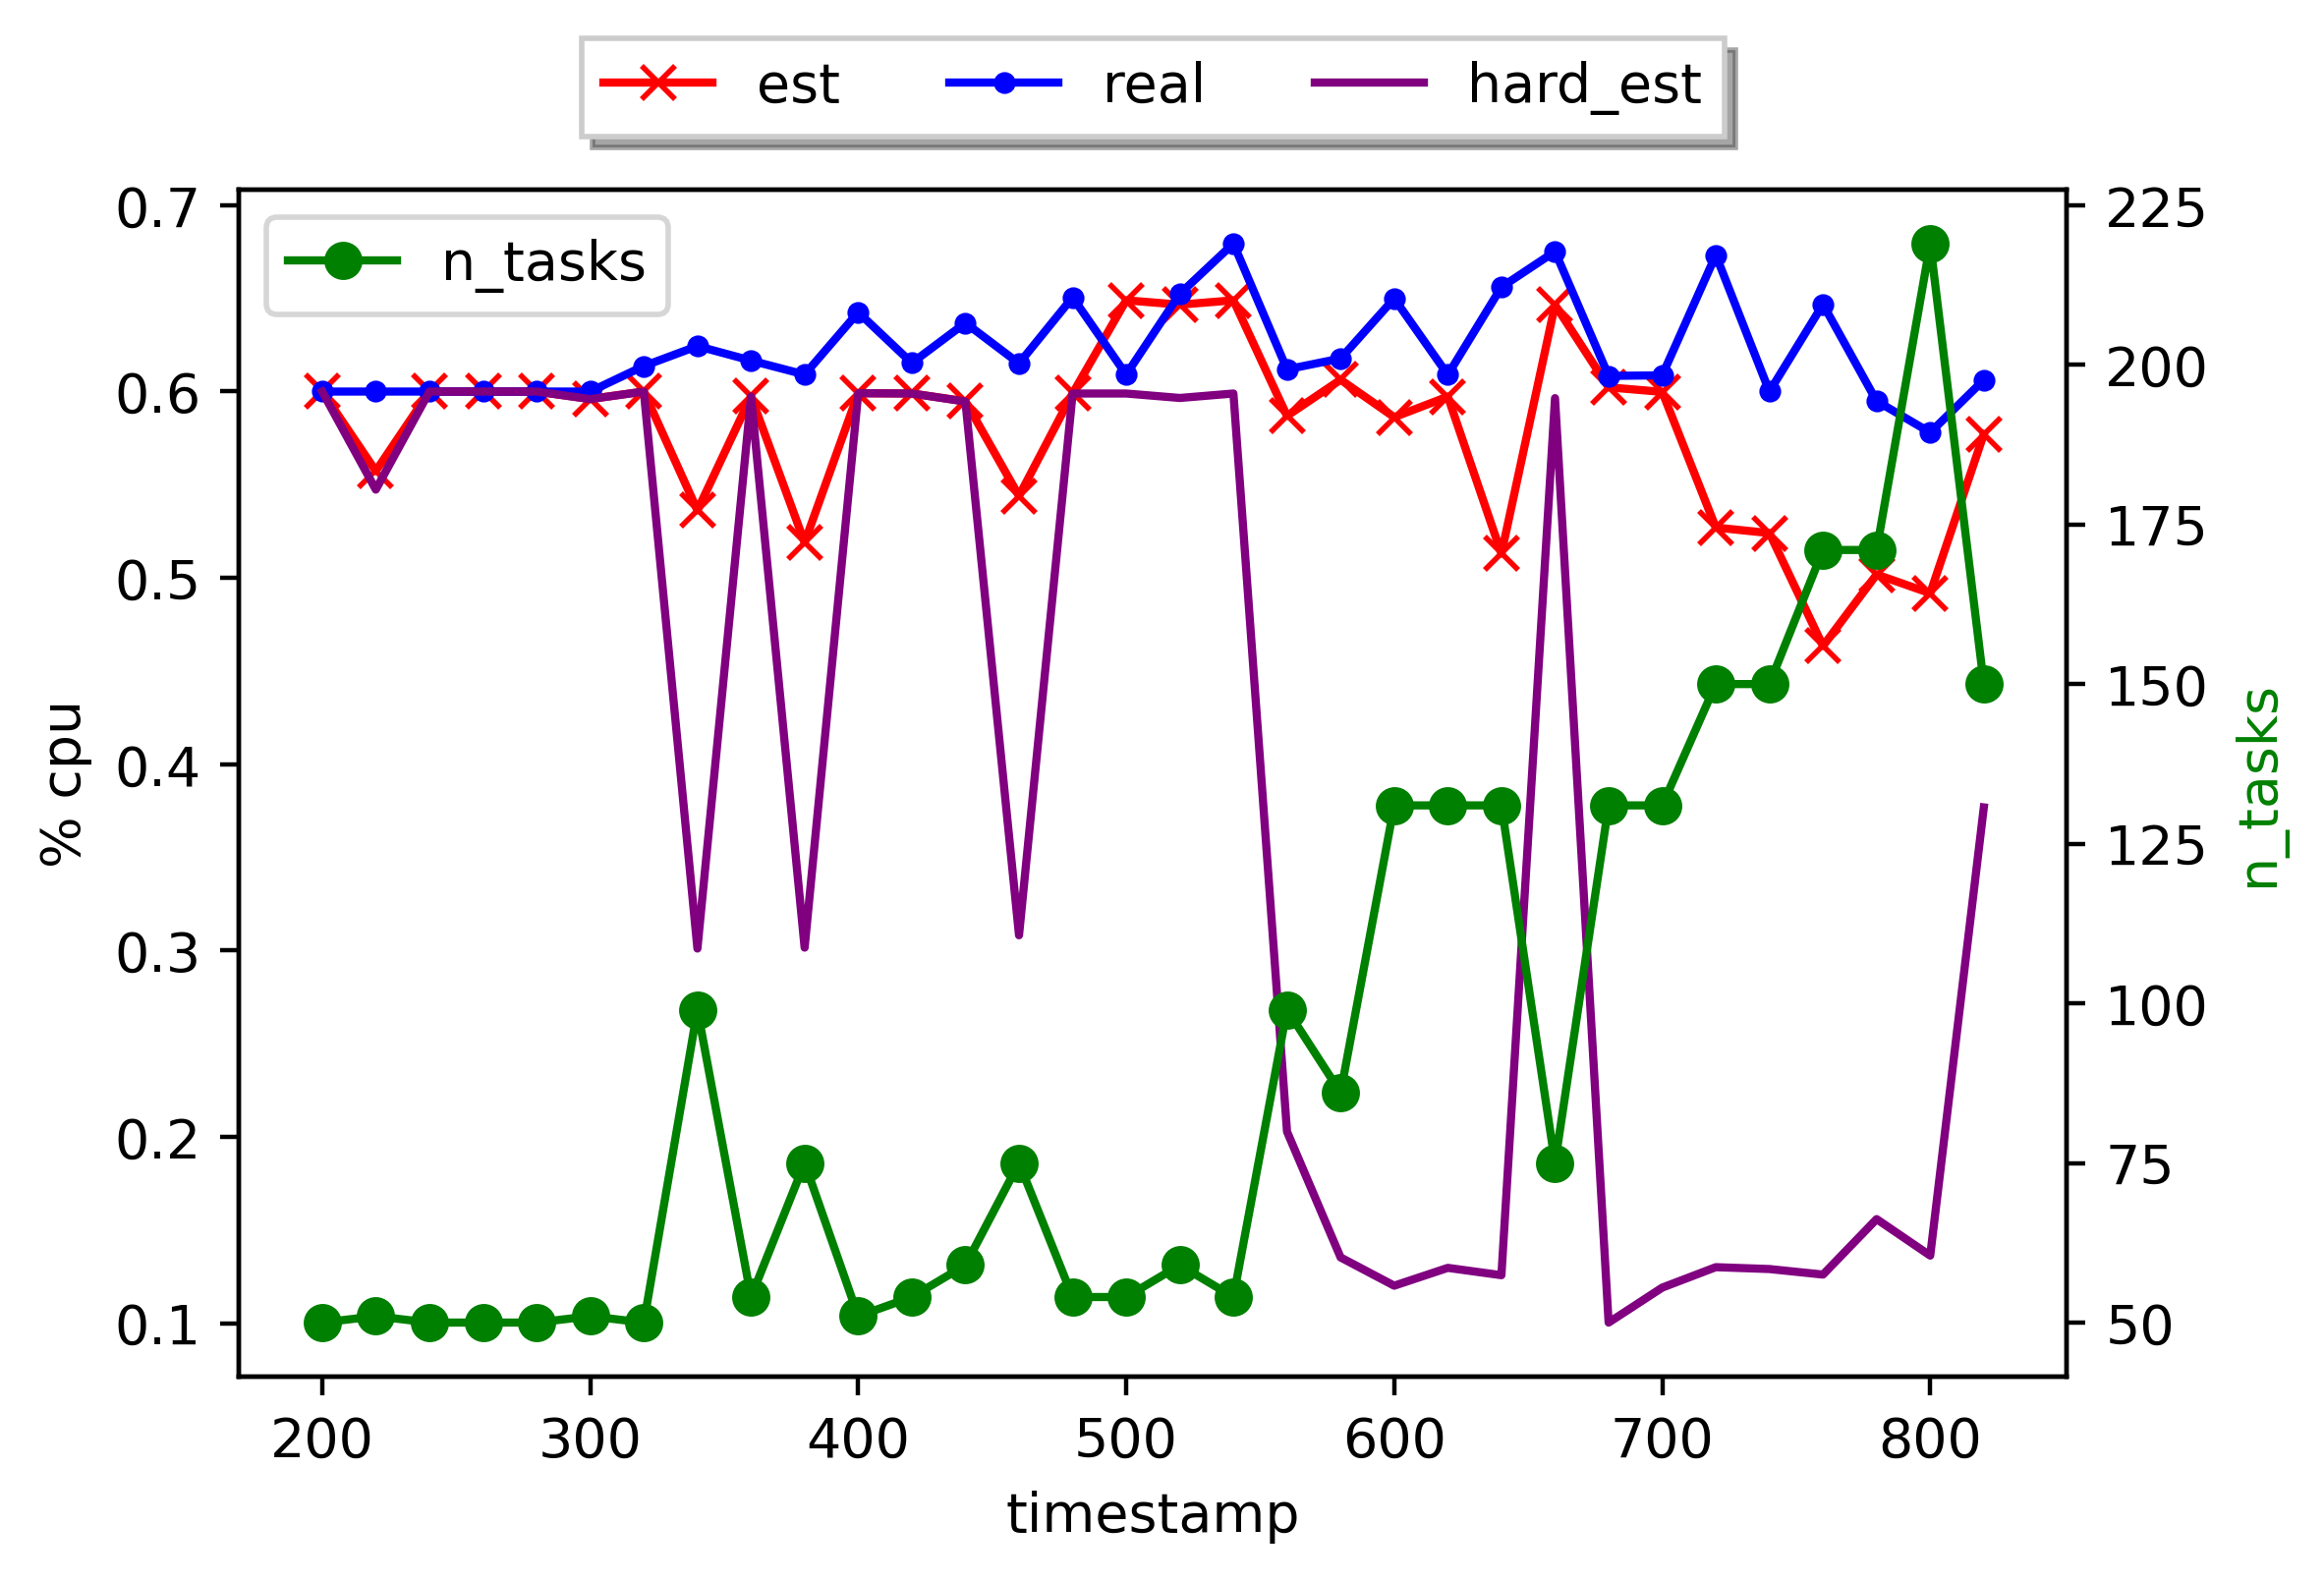
\includegraphics[width=.8\linewidth]{images/cpu_usage_estimation_2.png}
  \caption{Sai số với số lượng tasks đang chạy}
   \label{fig:usage_est_b}
\end{subfigure}
\end{figure}
\begin{center}
Mạng Bayesian cho kết quả ước lượng ({\color{red}{màu đỏ}}) có sai số với thực tế ({\color{blue}{màu xanh dương}}) nhỏ hơn so với việc dùng thông tin sai lệch ({\color{purple}{màu tím}}).
\end{center}
\end{frame}

\begin{frame}
{So sánh mức độ mất cân bằng giữa các máy tính}

\begin{minipage}[t]{0.4\linewidth}
	\vspace{0.5cm}
	\begin{itemize}
		\item Độ mất cân bằng giảm sâu tại thời điểm lập lịch (500, 520, ...) nhưng không duy trì được lâu 
		\item Thuật toán đề xuất cho độ mất cân bằng \textbf{ổn định và nhỏ hơn} so với Worstfit
	\end{itemize}
\end{minipage}
\hfill
\begin{minipage}[t]{0.59\linewidth}
	\begin{figure}[h!]
		\centering
		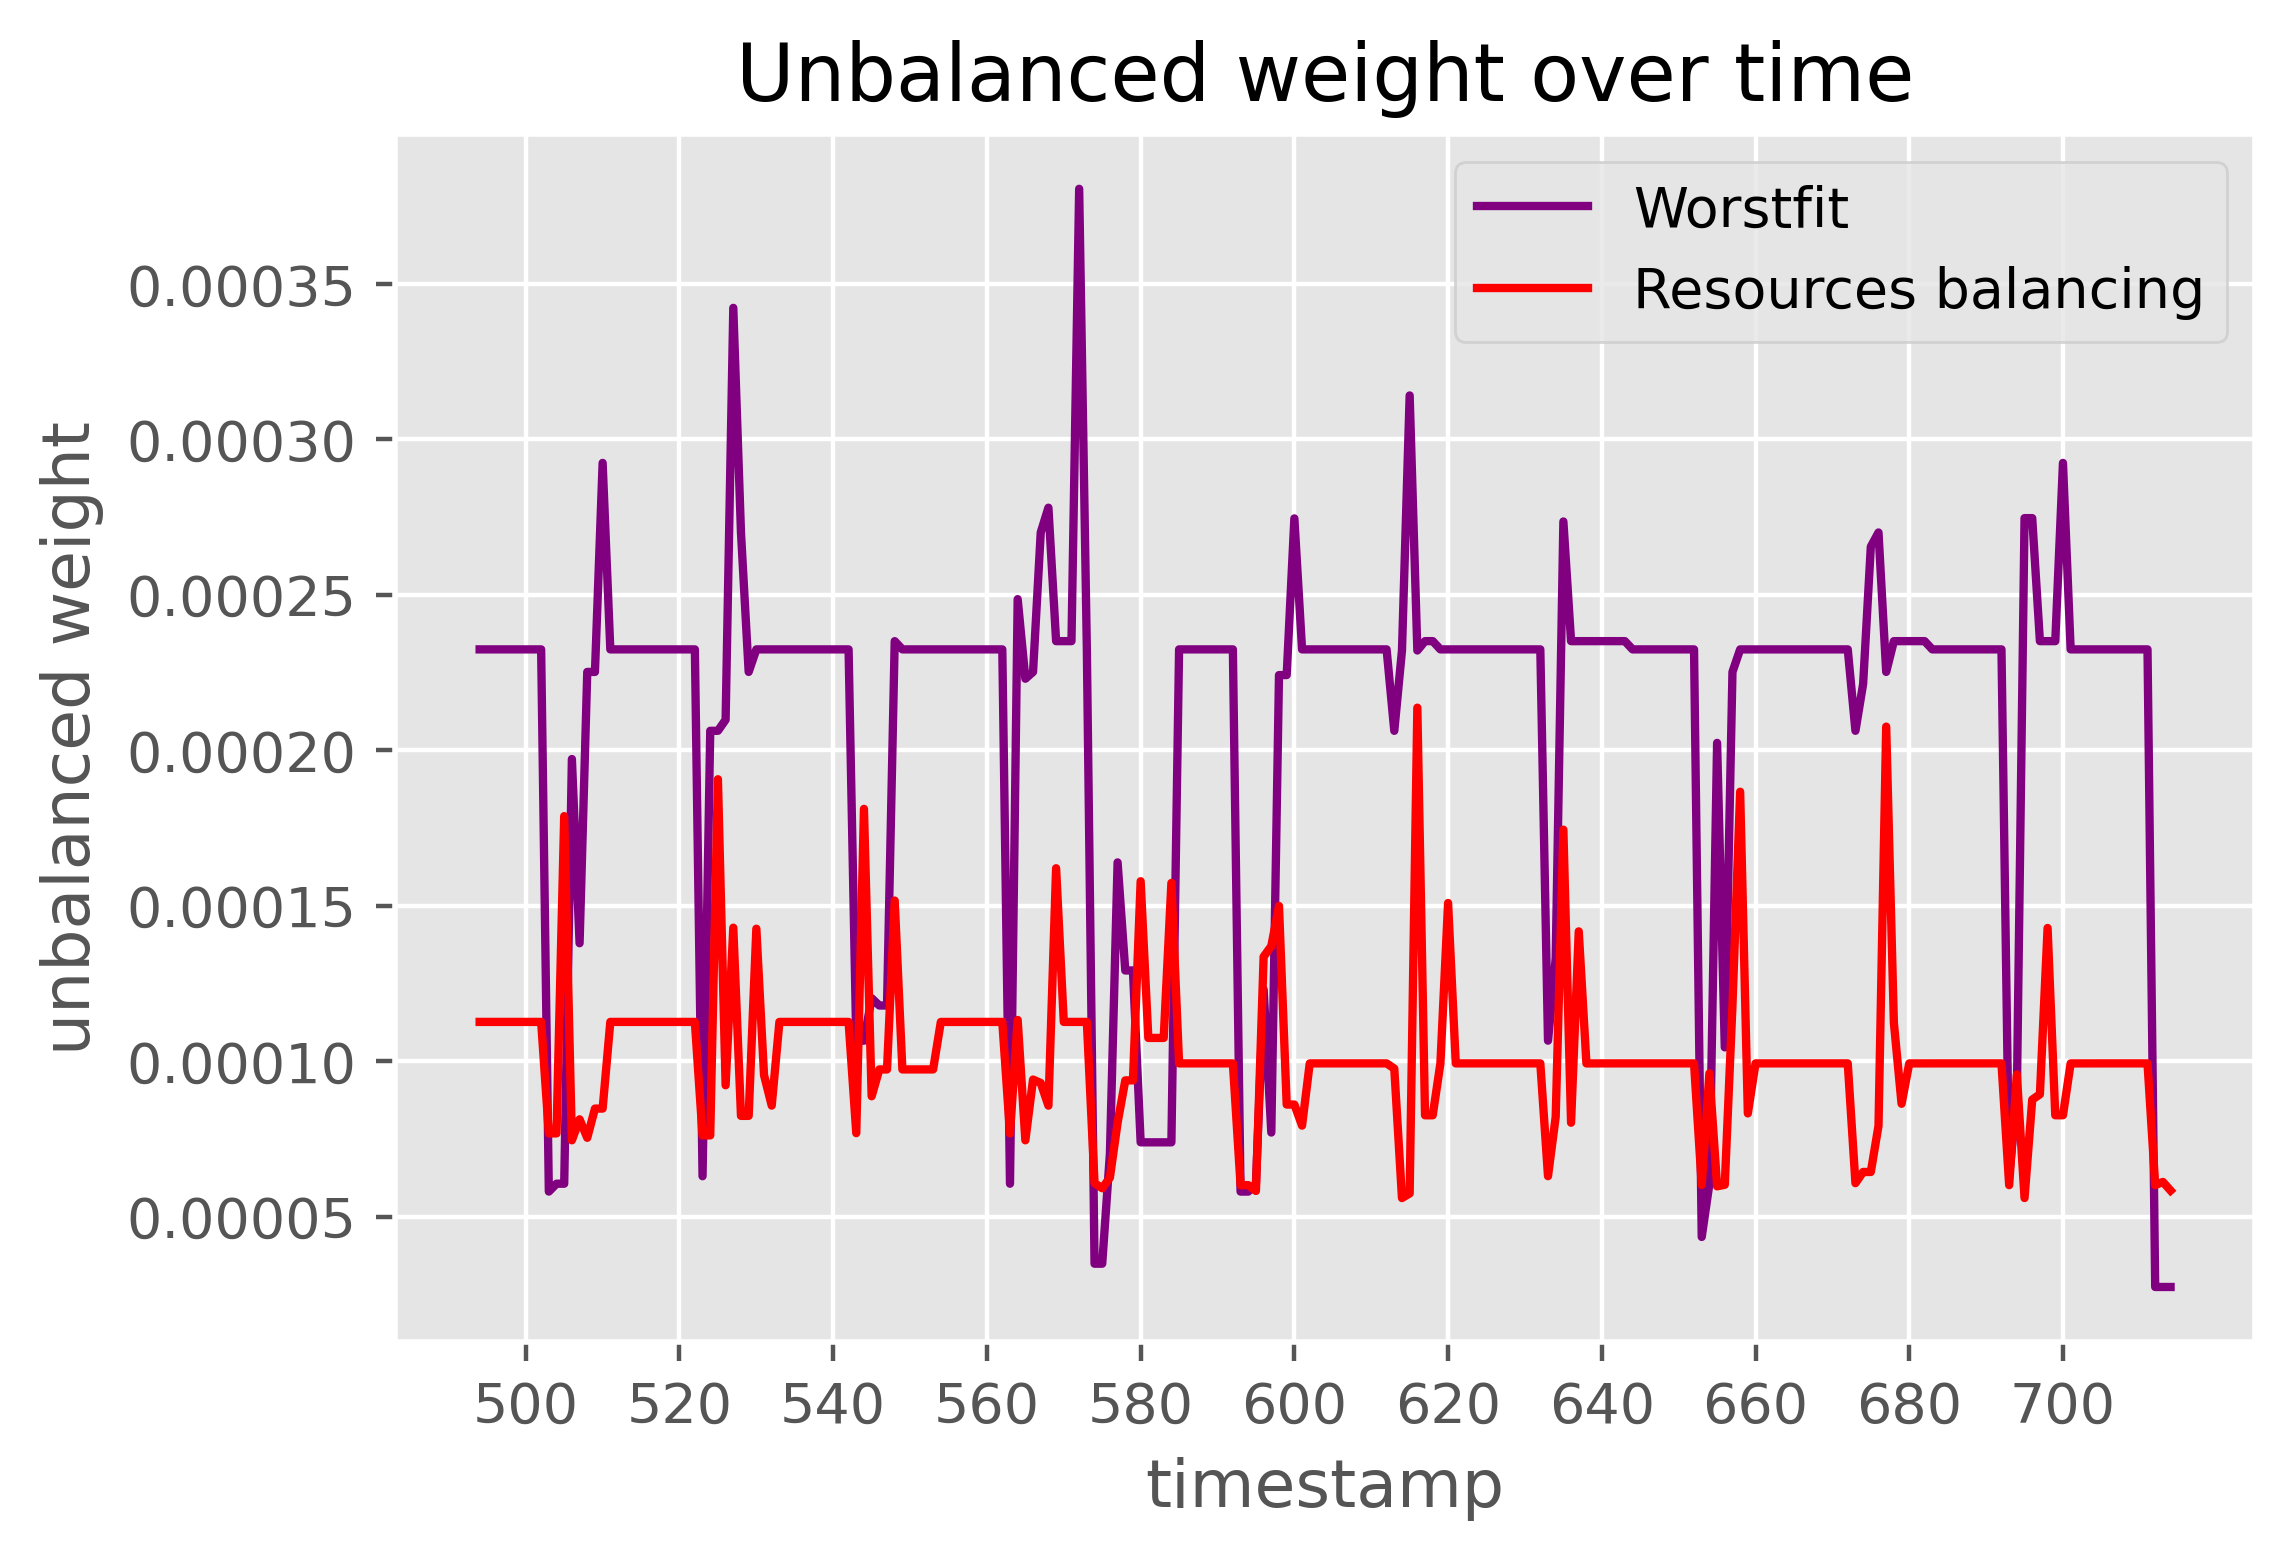
\includegraphics[scale=0.45]{images/unbalanced_weights.png}
		\caption{Độ mất cân bằng trong quá trình hoạt động}
	\end{figure}
\end{minipage}
\end{frame}

\section{Kết luận}

\begin{frame}
{Kết luận và định hướng}
% Trình bày kết quả đạt được 

\begin{block}
{Kết luận}
	\begin{itemize}
		\item Thuật toán đã cải thiện được sai số giữa thời điểm lập lịch và thực thi
		\item Có thể cân bằng được khối lượng công việc trong quá trình chạy 
	\end{itemize}
\end{block}

\pause
\begin{block}
{Định hướng phát triển}
\begin{itemize}
	\item Phát triển mô hình đồ thị Bayesian phù hợp với học liên tục 
	\item Mở rộng bài sang bài toán resource scaling
\end{itemize}
\end{block}
\end{frame}

{\1
\begin{frame}[plain,noframenumbering]
  \finalpage{\Large\textit{Em xin trân thành cảm ơn Thầy cô và mọi người đã lắng nghe}}
\end{frame}}

\end{document}